\documentclass{article}
\usepackage[UTF8]{ctex}
\usepackage{geometry}
\usepackage{makecell}
\usepackage{amsmath}
\usepackage{graphicx}
\usepackage{bigstrut}
\usepackage{subfigure}
\usepackage{float}

\geometry{a4paper,scale=0.75}

\title{\heiti 实验三十五\  阿贝成像原理和空间滤波}
\author{\kaishu 田睿轩\ 物理学院\ 1900011602}
\date{2021年4月8日}
\newcommand{\degree}{^\circ}
\newcommand{\degreesCelsius}{^\circ C}

\begin{document}
    \maketitle
    \section{数据处理}
    \subsection{一维光栅}
    \subsubsection{空间频率测量}
    在透镜的后焦面(即频谱面)上放上半透的屏,可以看到沿水平方向分布的衍射光斑。然后利用读数显微镜在其后测量频谱面上各衍射光点的位置。
    测量时从0级衍射点开始测量,分别向左和向右测量1级、2级、3级衍射点在读数尺上的坐标,计算出到0级衍射的距离,
    然后将向左和向右测量的结果取平均作为不同级衍射点到0级衍射点的距离。实验数据如下表:
    \begin{table}[h]
        \begin{minipage}{0.49\textwidth}
            \centering
            \begin{tabular}{|c|c|c|}
                \hline
                衍射级次 & 位置$x'/mm$ & 距离$\Delta x'/mm$ \\
                \hline
                0 & 28.689 & 0.000 \\
                \hline
                +1 & 30.618 & 1.929 \\
                \hline
                +2 & 32.595 & 3.886 \\
                \hline
                +3 & 34.437 & 5.748 \\
                \hline
            \end{tabular}
            \caption{向右测量各衍射斑点到0级衍射的距离}
        \end{minipage}
        \begin{minipage}{0.49\textwidth}
            \centering
            \begin{tabular}{|c|c|c|}
                \hline
                衍射级次 & 位置$x'/mm$ & 距离$\Delta x'/mm$ \\
                \hline
                0 &  28.662  & 0.000 \\
                \hline
                -1 & 26.809 & 1.853 \\
                \hline
                -2 & 24.893 & 3.789 \\
                \hline
                -3 & 22.968 & 5.694 \\
                \hline
            \end{tabular}
            \caption{向左测量各衍射斑点到0级衍射的距离}
        \end{minipage}
    \end{table}

    利用公式$f=\frac{\Delta x'}{\lambda F}$可计算相应的空间频率,其中$\lambda$为激光波长,
    为632.8nm,$F$为透镜焦距,取为25cm,计算结果如下

    \begin{table}[h]
        \centering
        \begin{tabular}{|c|c|c|}
            \hline
            级次 & $\bar{\Delta x'}/mm$ & 空间频率$f/mm^{-1}$ \\
            \hline
            1 & 1.891 & 11.96 \\
            \hline
            2 & 3.838 & 24.26 \\
            \hline
            3 & 3.721 & 36.16\\
            \hline
        \end{tabular}
        \caption{各级次空间频率}
    \end{table}

    因此,该光栅的基频为$11.96mm^{-1}$。

    \subsubsection{空间滤波实验}

    \begin{enumerate}
        \item [(1)] 全通过 \\
        \begin{table}[htb]
            \centering
            \begin{tabular}{|c|c|c|c|}
                \hline
                通过的点 & 起点位置$x/mm$ & 10个条纹后的位置$x'/mm$ & 条纹间距$d/mm$ \\
                \hline
                全部 & 42.238 & 37.112 & 0.5126 \\
                \hline
            \end{tabular}
            \caption{条纹间距测量结果}
        \end{table}
        \begin{figure*}[htb]
            \centering
            \subfigure[光屏上的像]{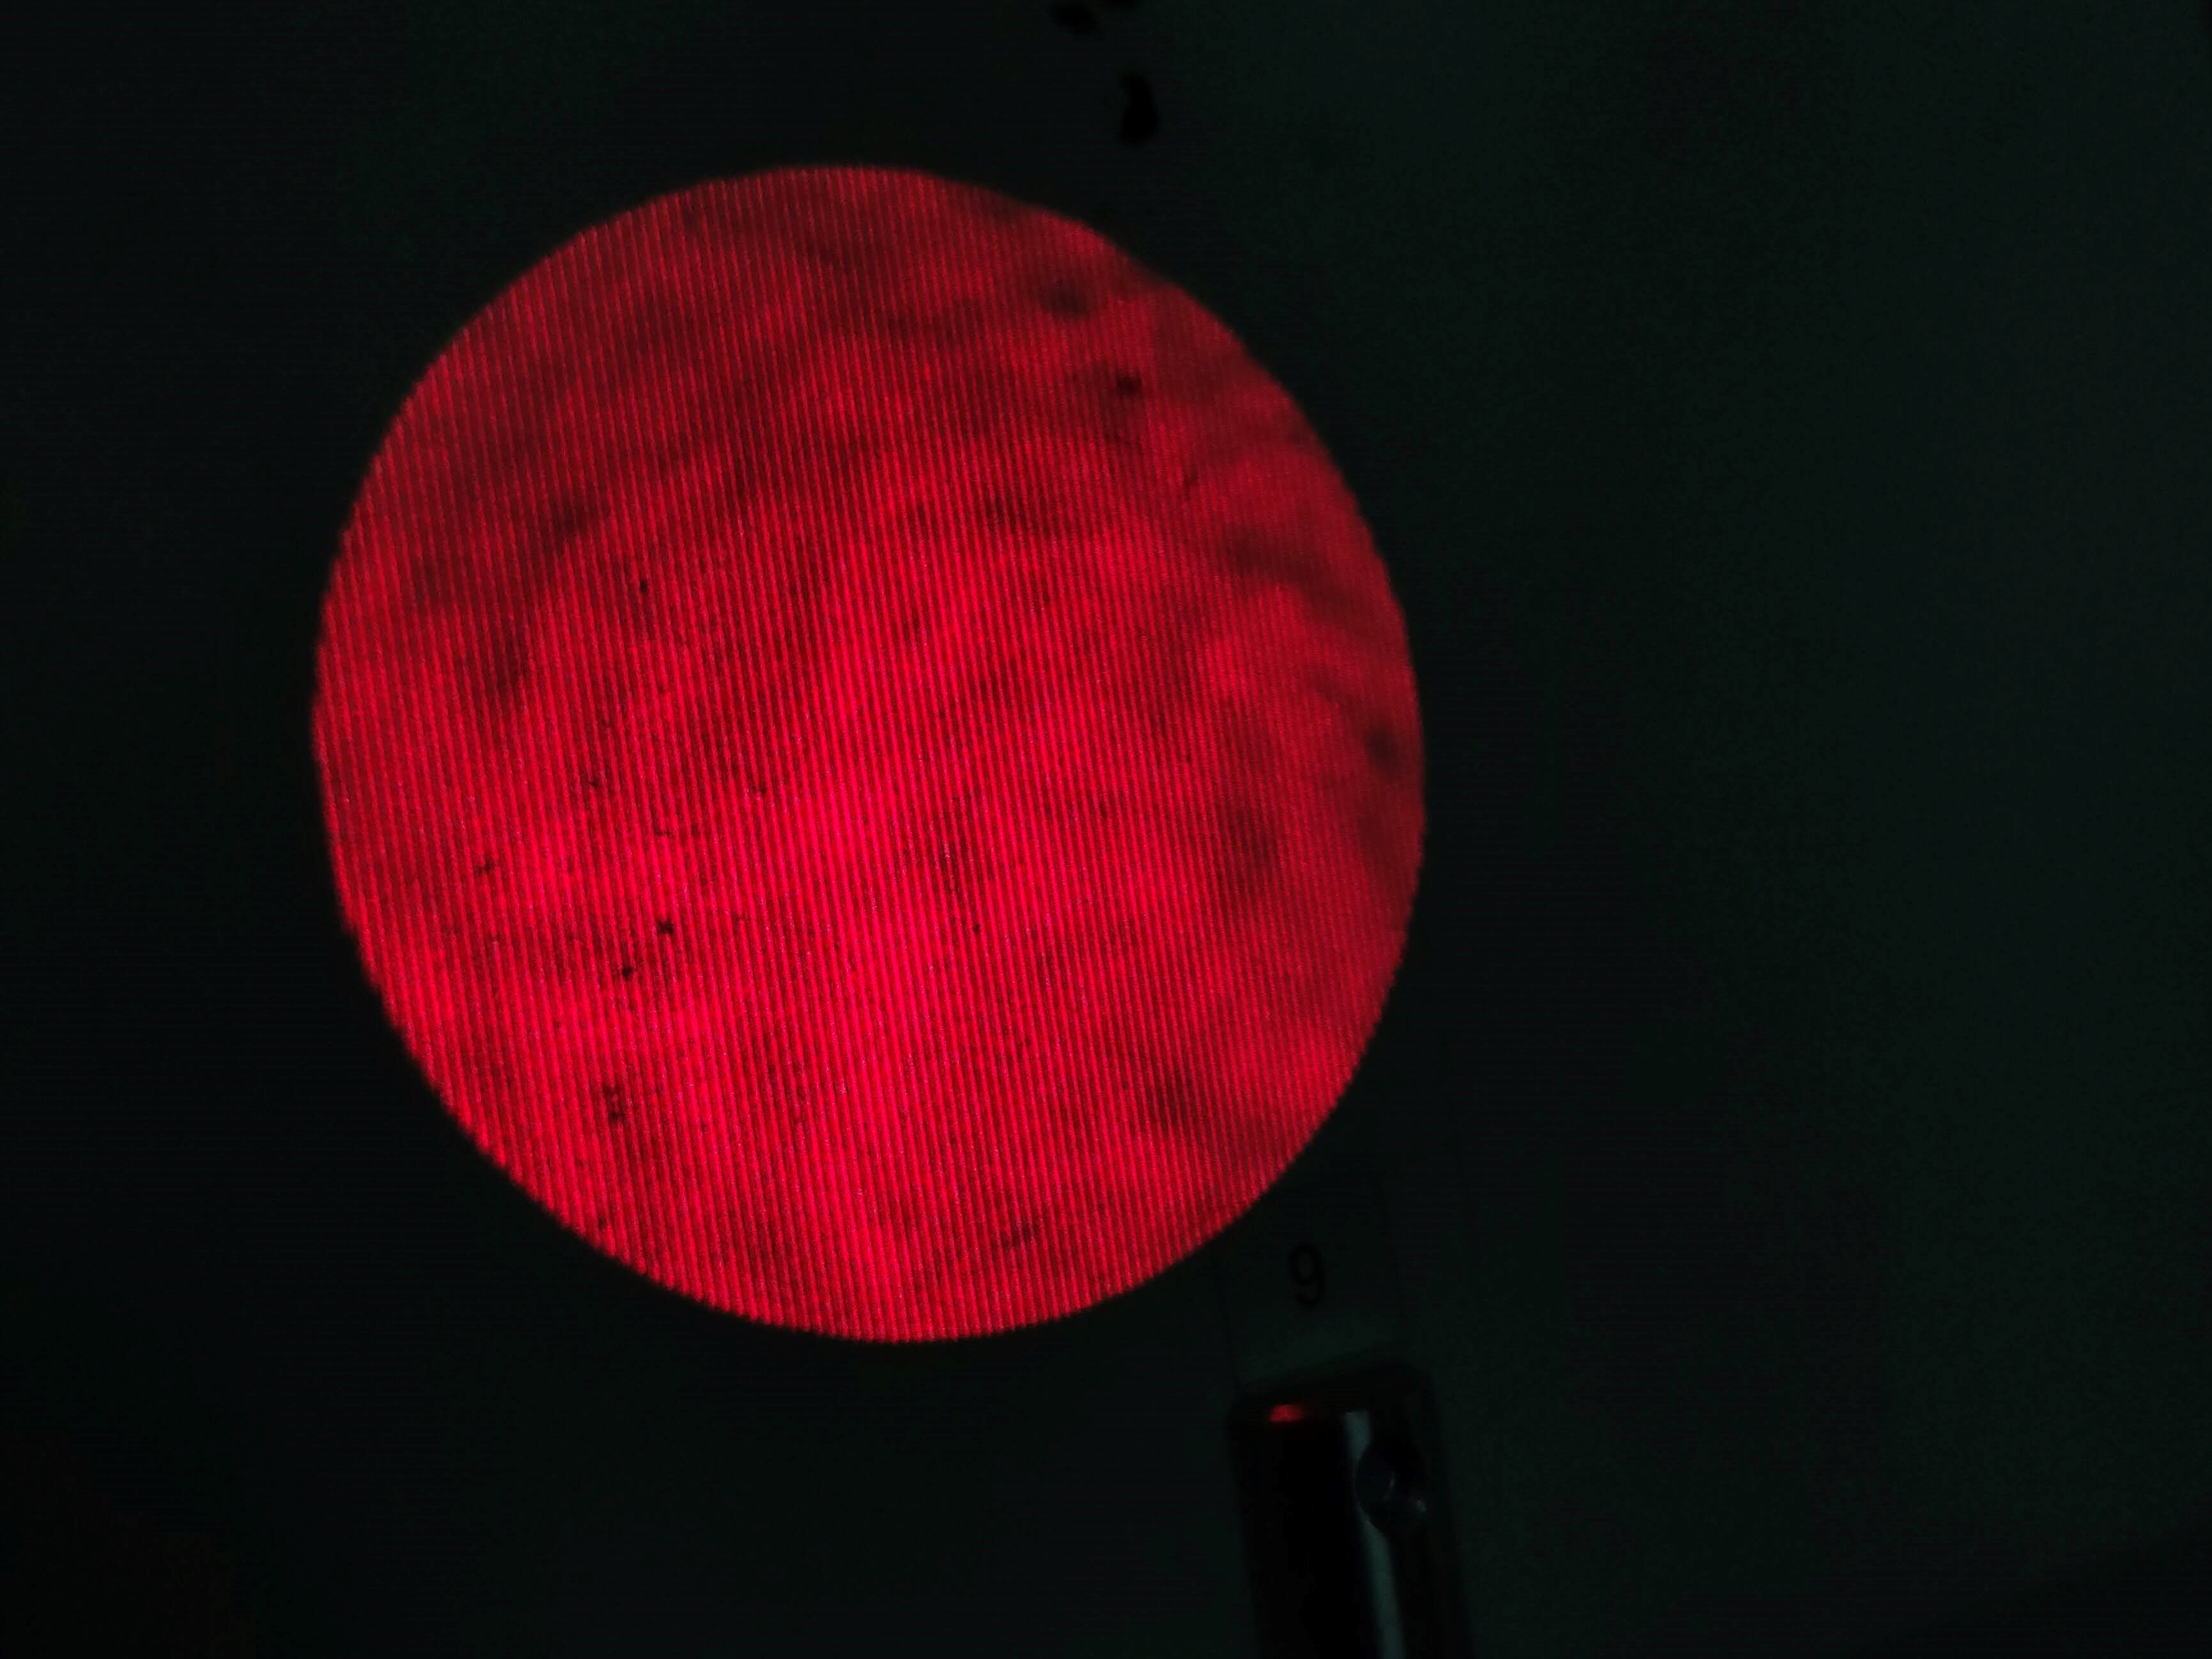
\includegraphics[width=0.45\textwidth]{一维-全通过-屏.jpg}}
            \subfigure[显微镜中的像]{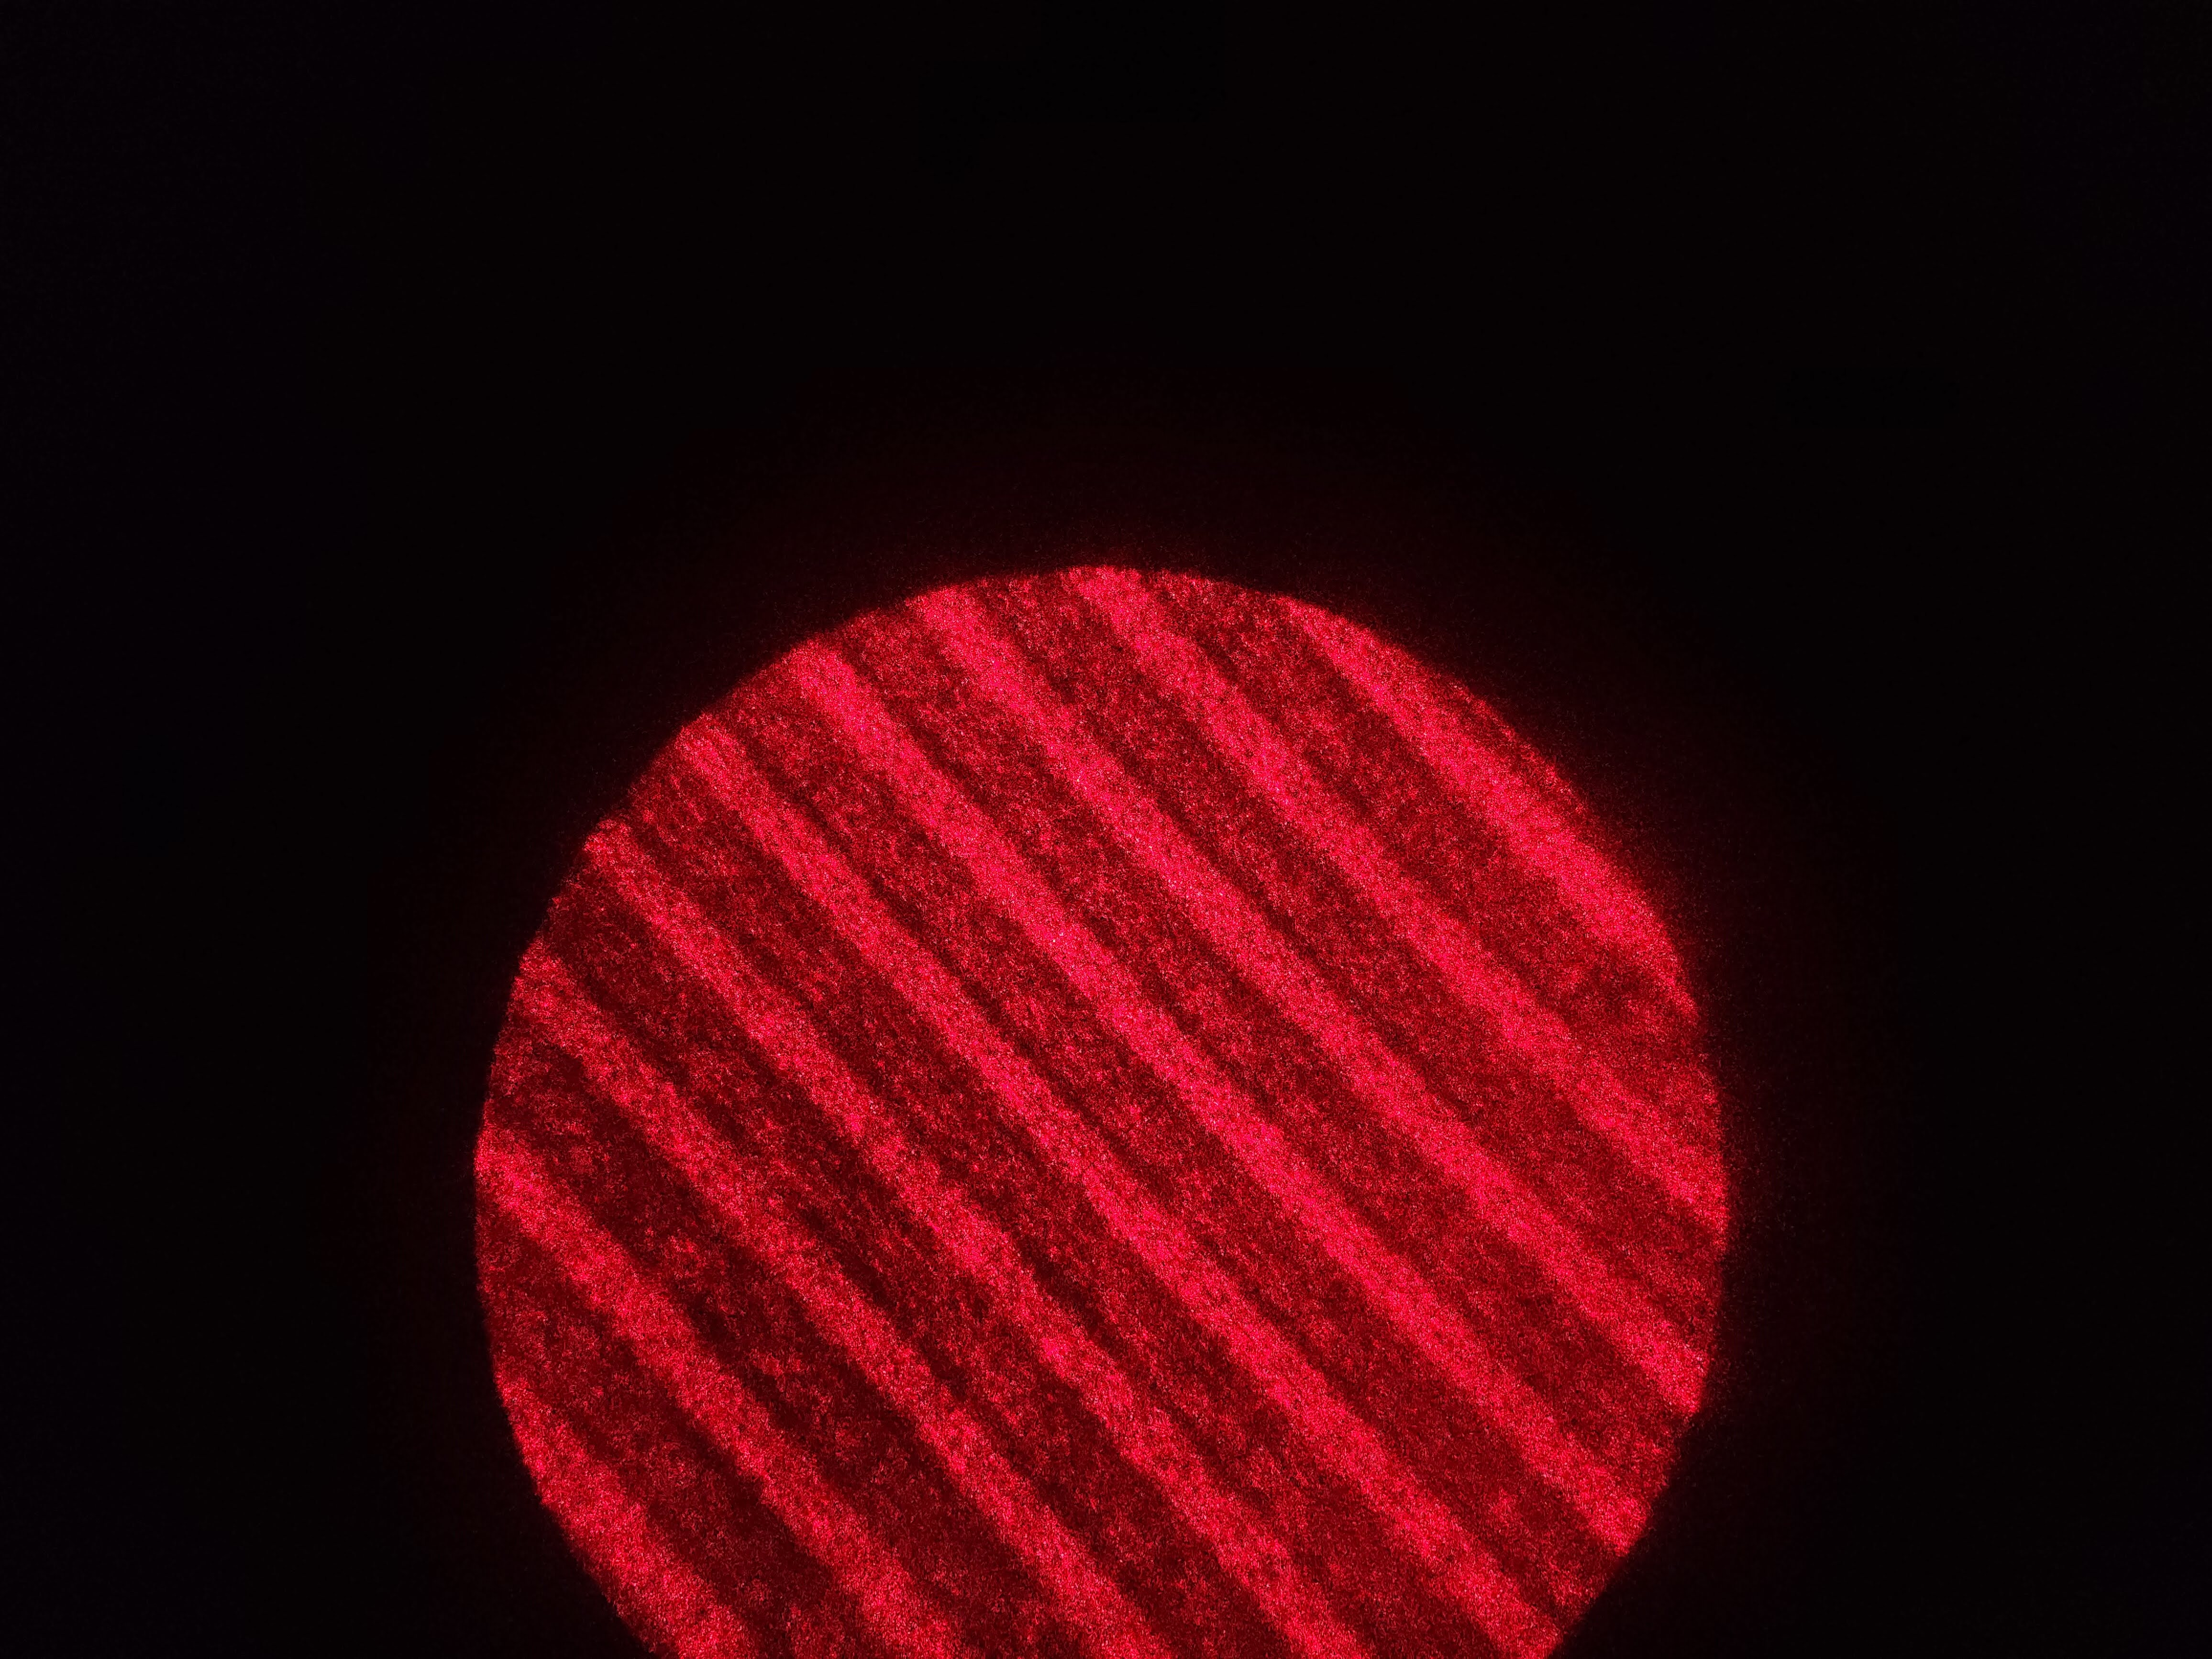
\includegraphics[width=0.45\textwidth]{一维-全通过-显微镜.jpg}}
            \caption{通过0级}
        \end{figure*}

        根据焦距公式和物距、焦距计算出像距,将光屏放在附近寻找最清晰的位置,然后用半透明的玻璃作为屏,用显微镜在后面观察并读数。
        如图1所示,光屏上和显微镜中均能看到清晰的纵向条纹。条纹间距测量结果如表4所示。

        \item [(2)] 通过0级衍射点 \\
        \begin{figure*}[htb]
            \centering
            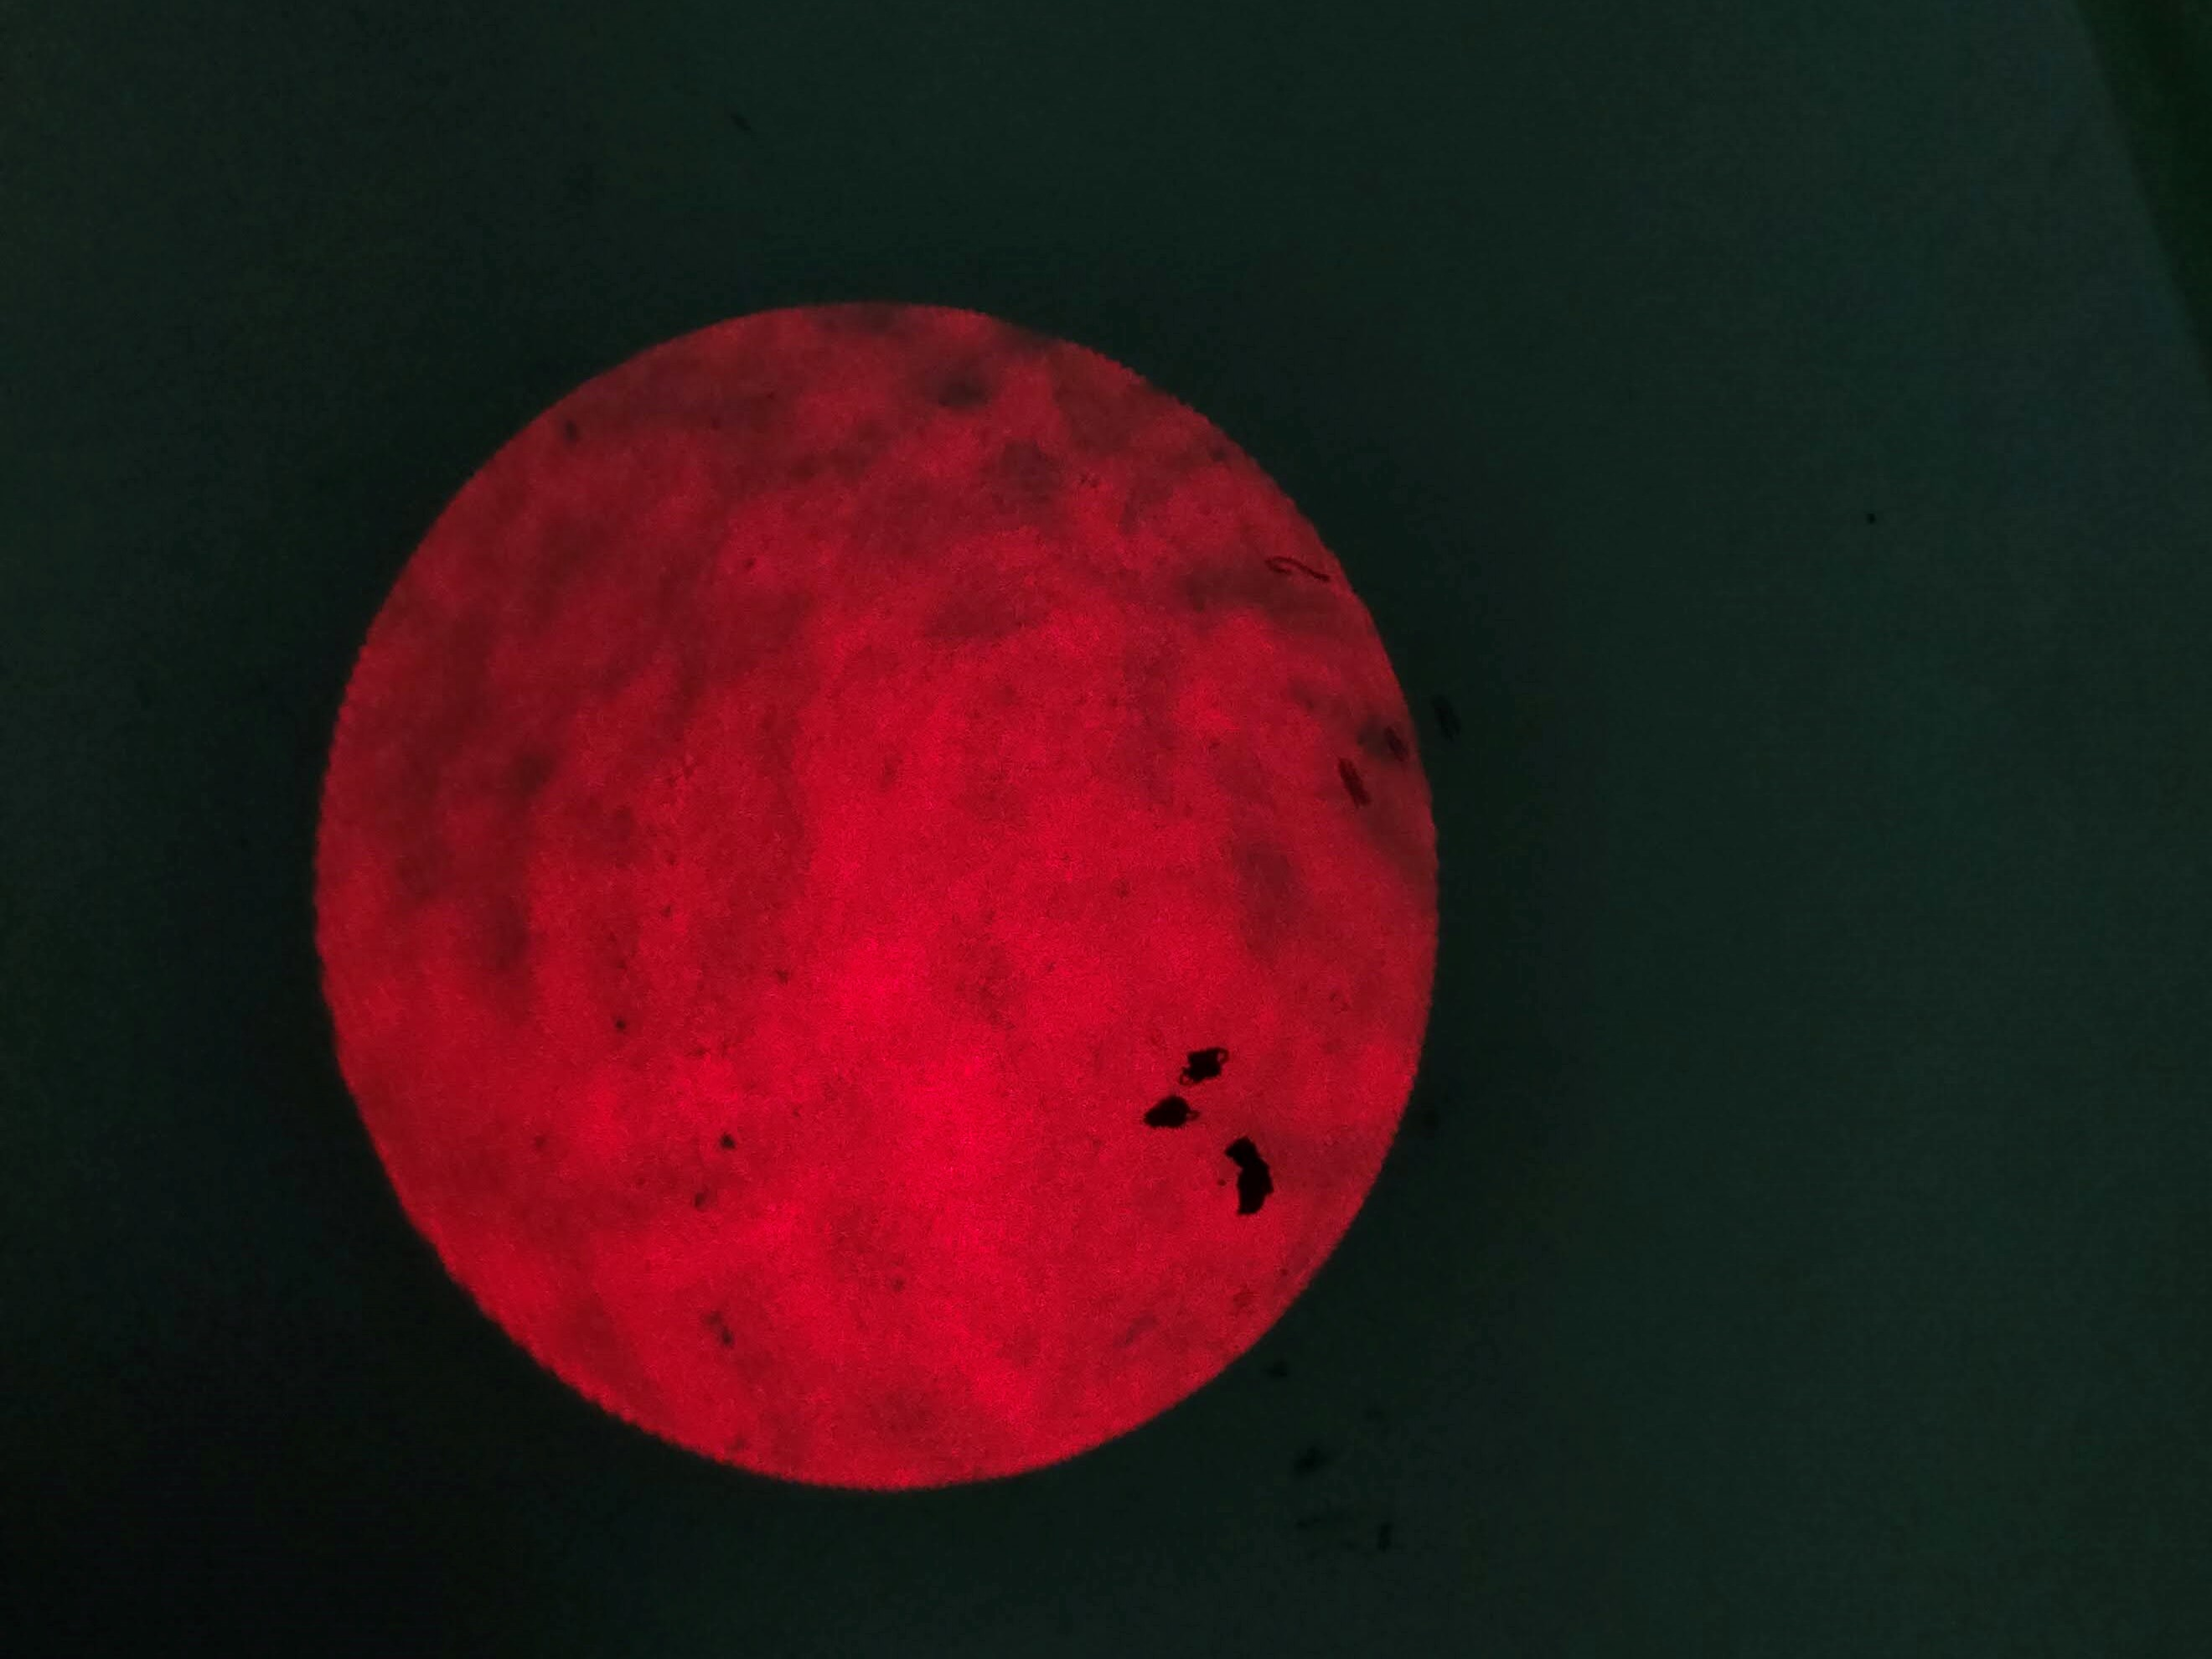
\includegraphics[width=0.45\textwidth]{一维-0级通-屏.jpg}
            \caption{只通过0级衍射点}
        \end{figure*}
        
        将频谱面上的衍射光斑除0级外的都挡住,只允许0级衍射点通过。结果如图2,可以看到只能看到均匀的红色的一片,没有任何条纹。
        这是因为0级衍射点不包括任何细节信息,因此只允许0级衍射点通过的情况下,物的所有细节情况都被滤除,
        因此也就看不到任何条纹细节。由于看不到条纹,自然无法测量条纹间距。

        \item [(3)] 通过0级,$\pm 1$级 \\
        \begin{table}[htb]
            \centering
            \begin{tabular}{|c|c|c|c|}
                \hline
                通过的点 & 起点位置$x/mm$ & 10个条纹后的位置$x'/mm$ & 条纹间距$d/mm$ \\
                \hline
                全部 & 35.925 & 41.148 & 0.5223 \\
                \hline
            \end{tabular}
            \caption{条纹间距测量结果}
        \end{table}
        \begin{figure*}[htb]
            \centering
            \subfigure[光屏上的像]{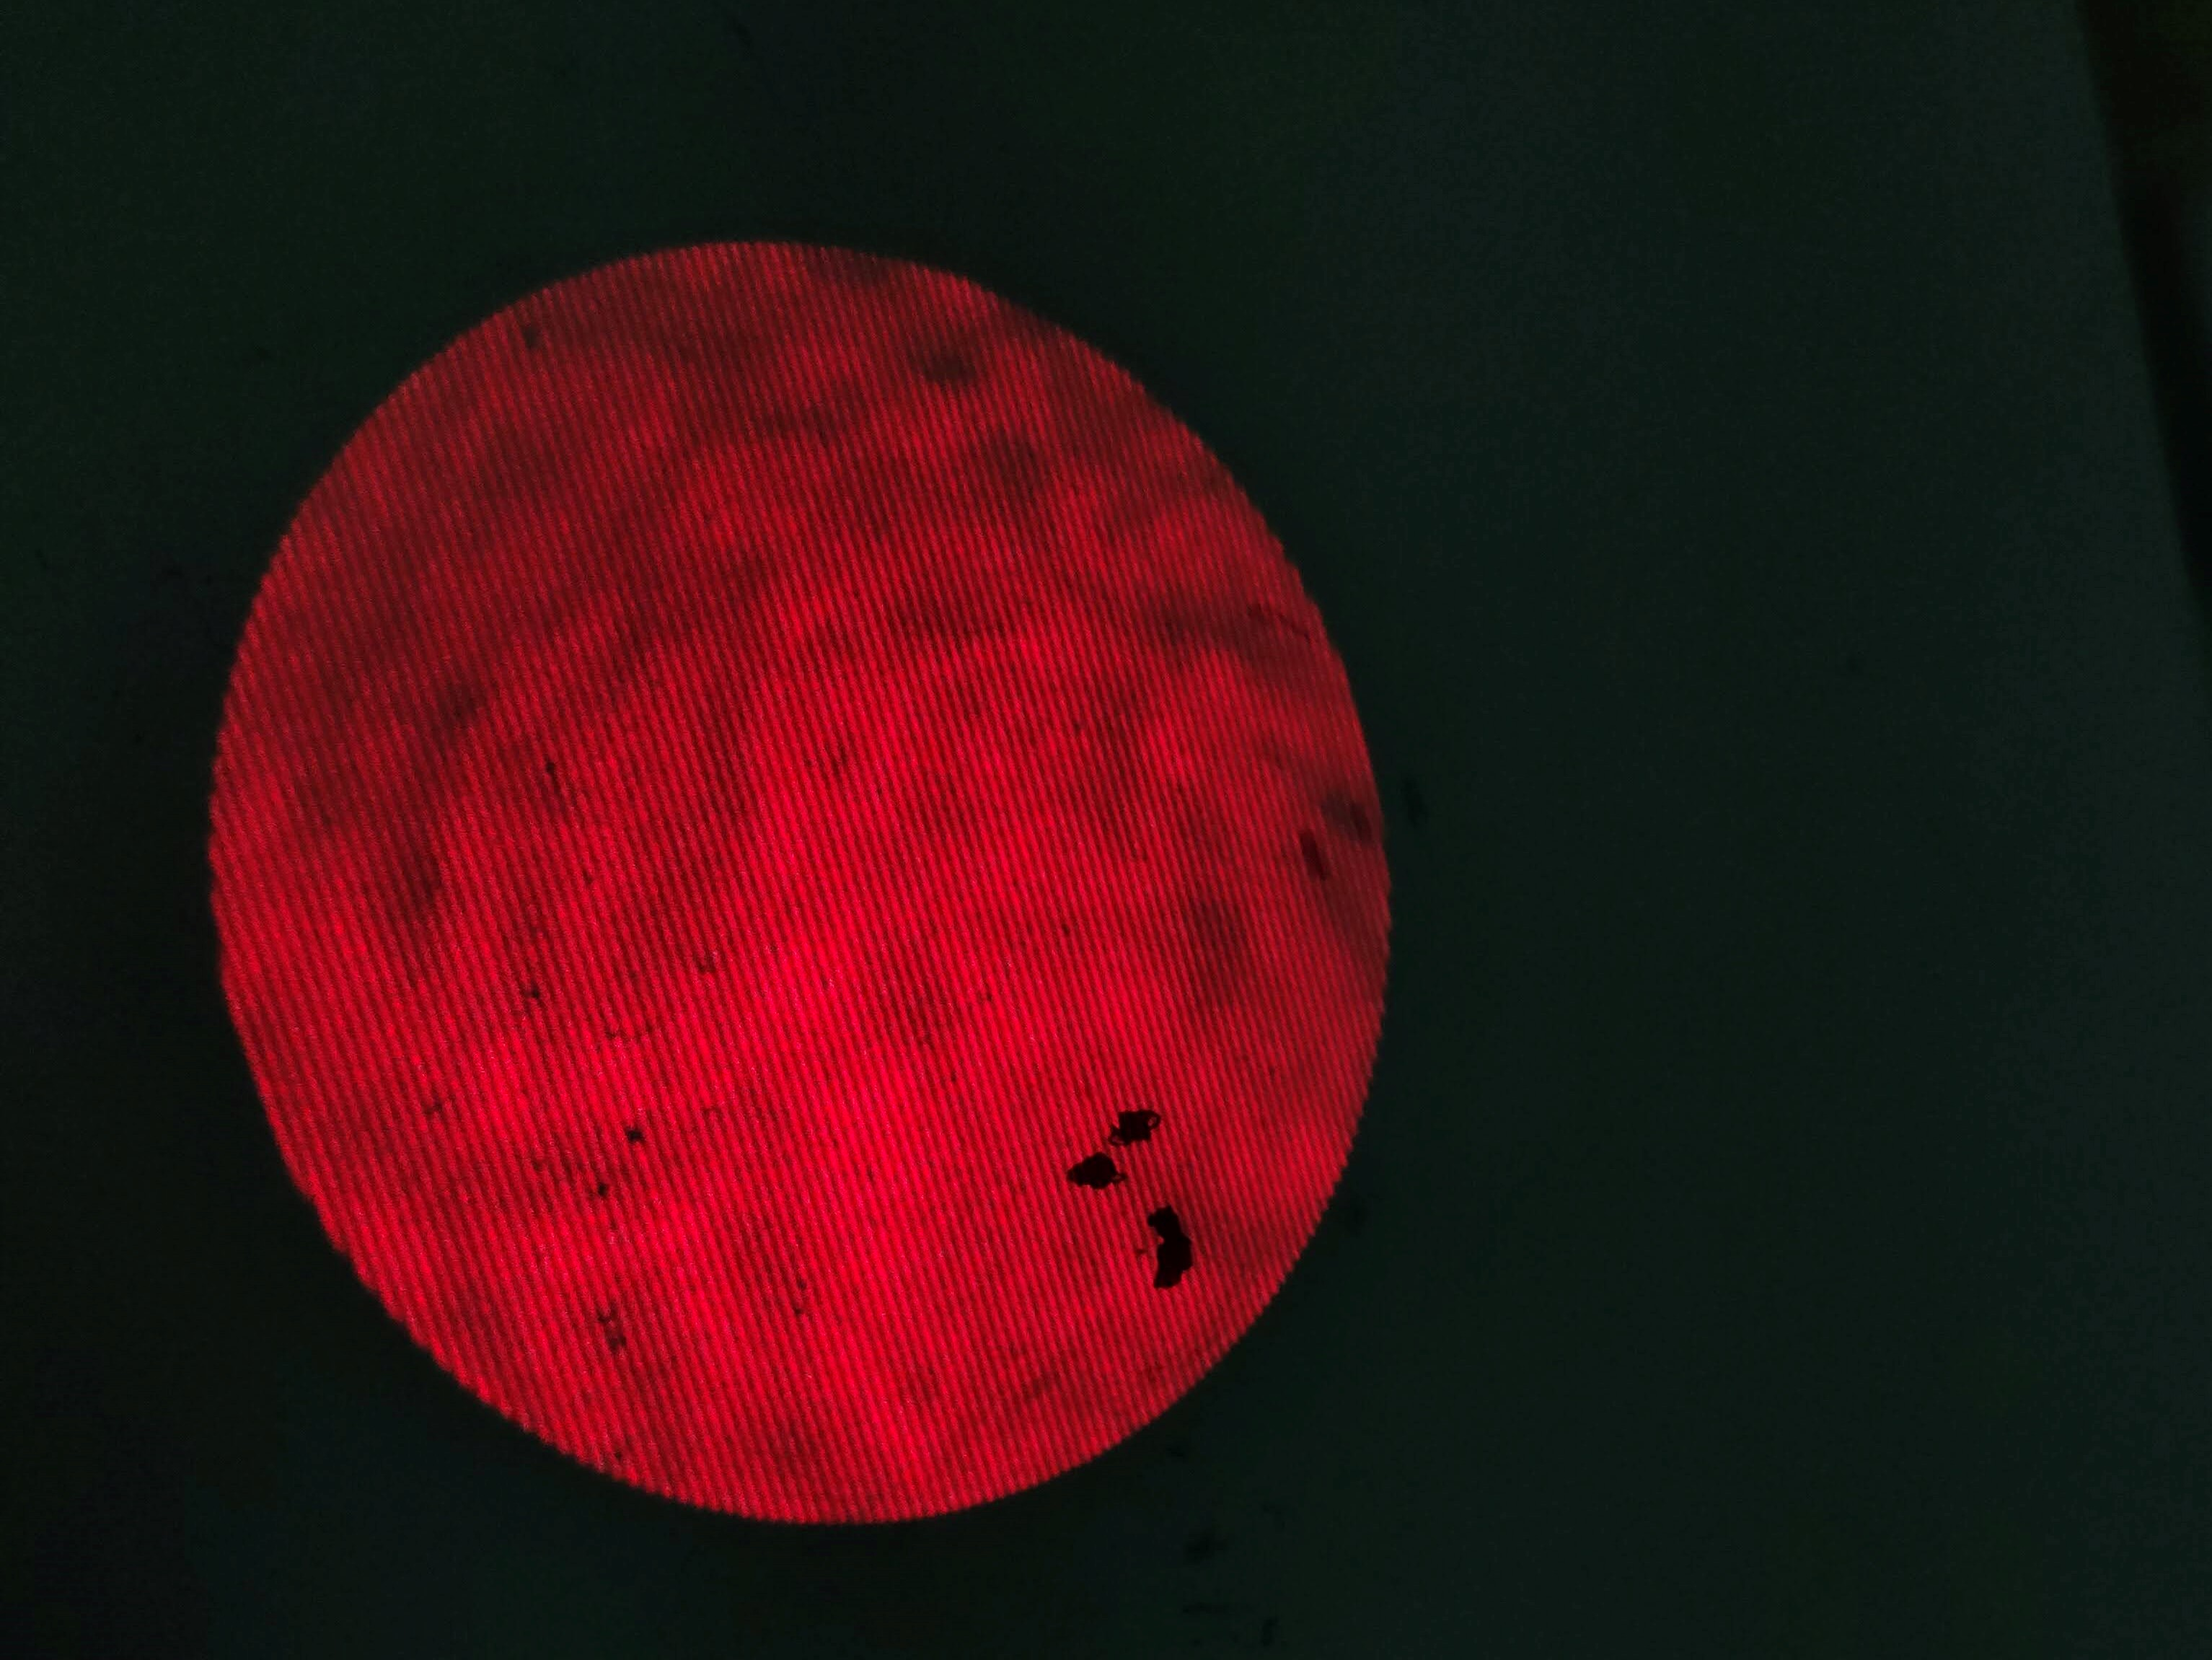
\includegraphics[width=0.45\textwidth]{一维-0级1级-屏.jpg}}
            \subfigure[显微镜中的像]{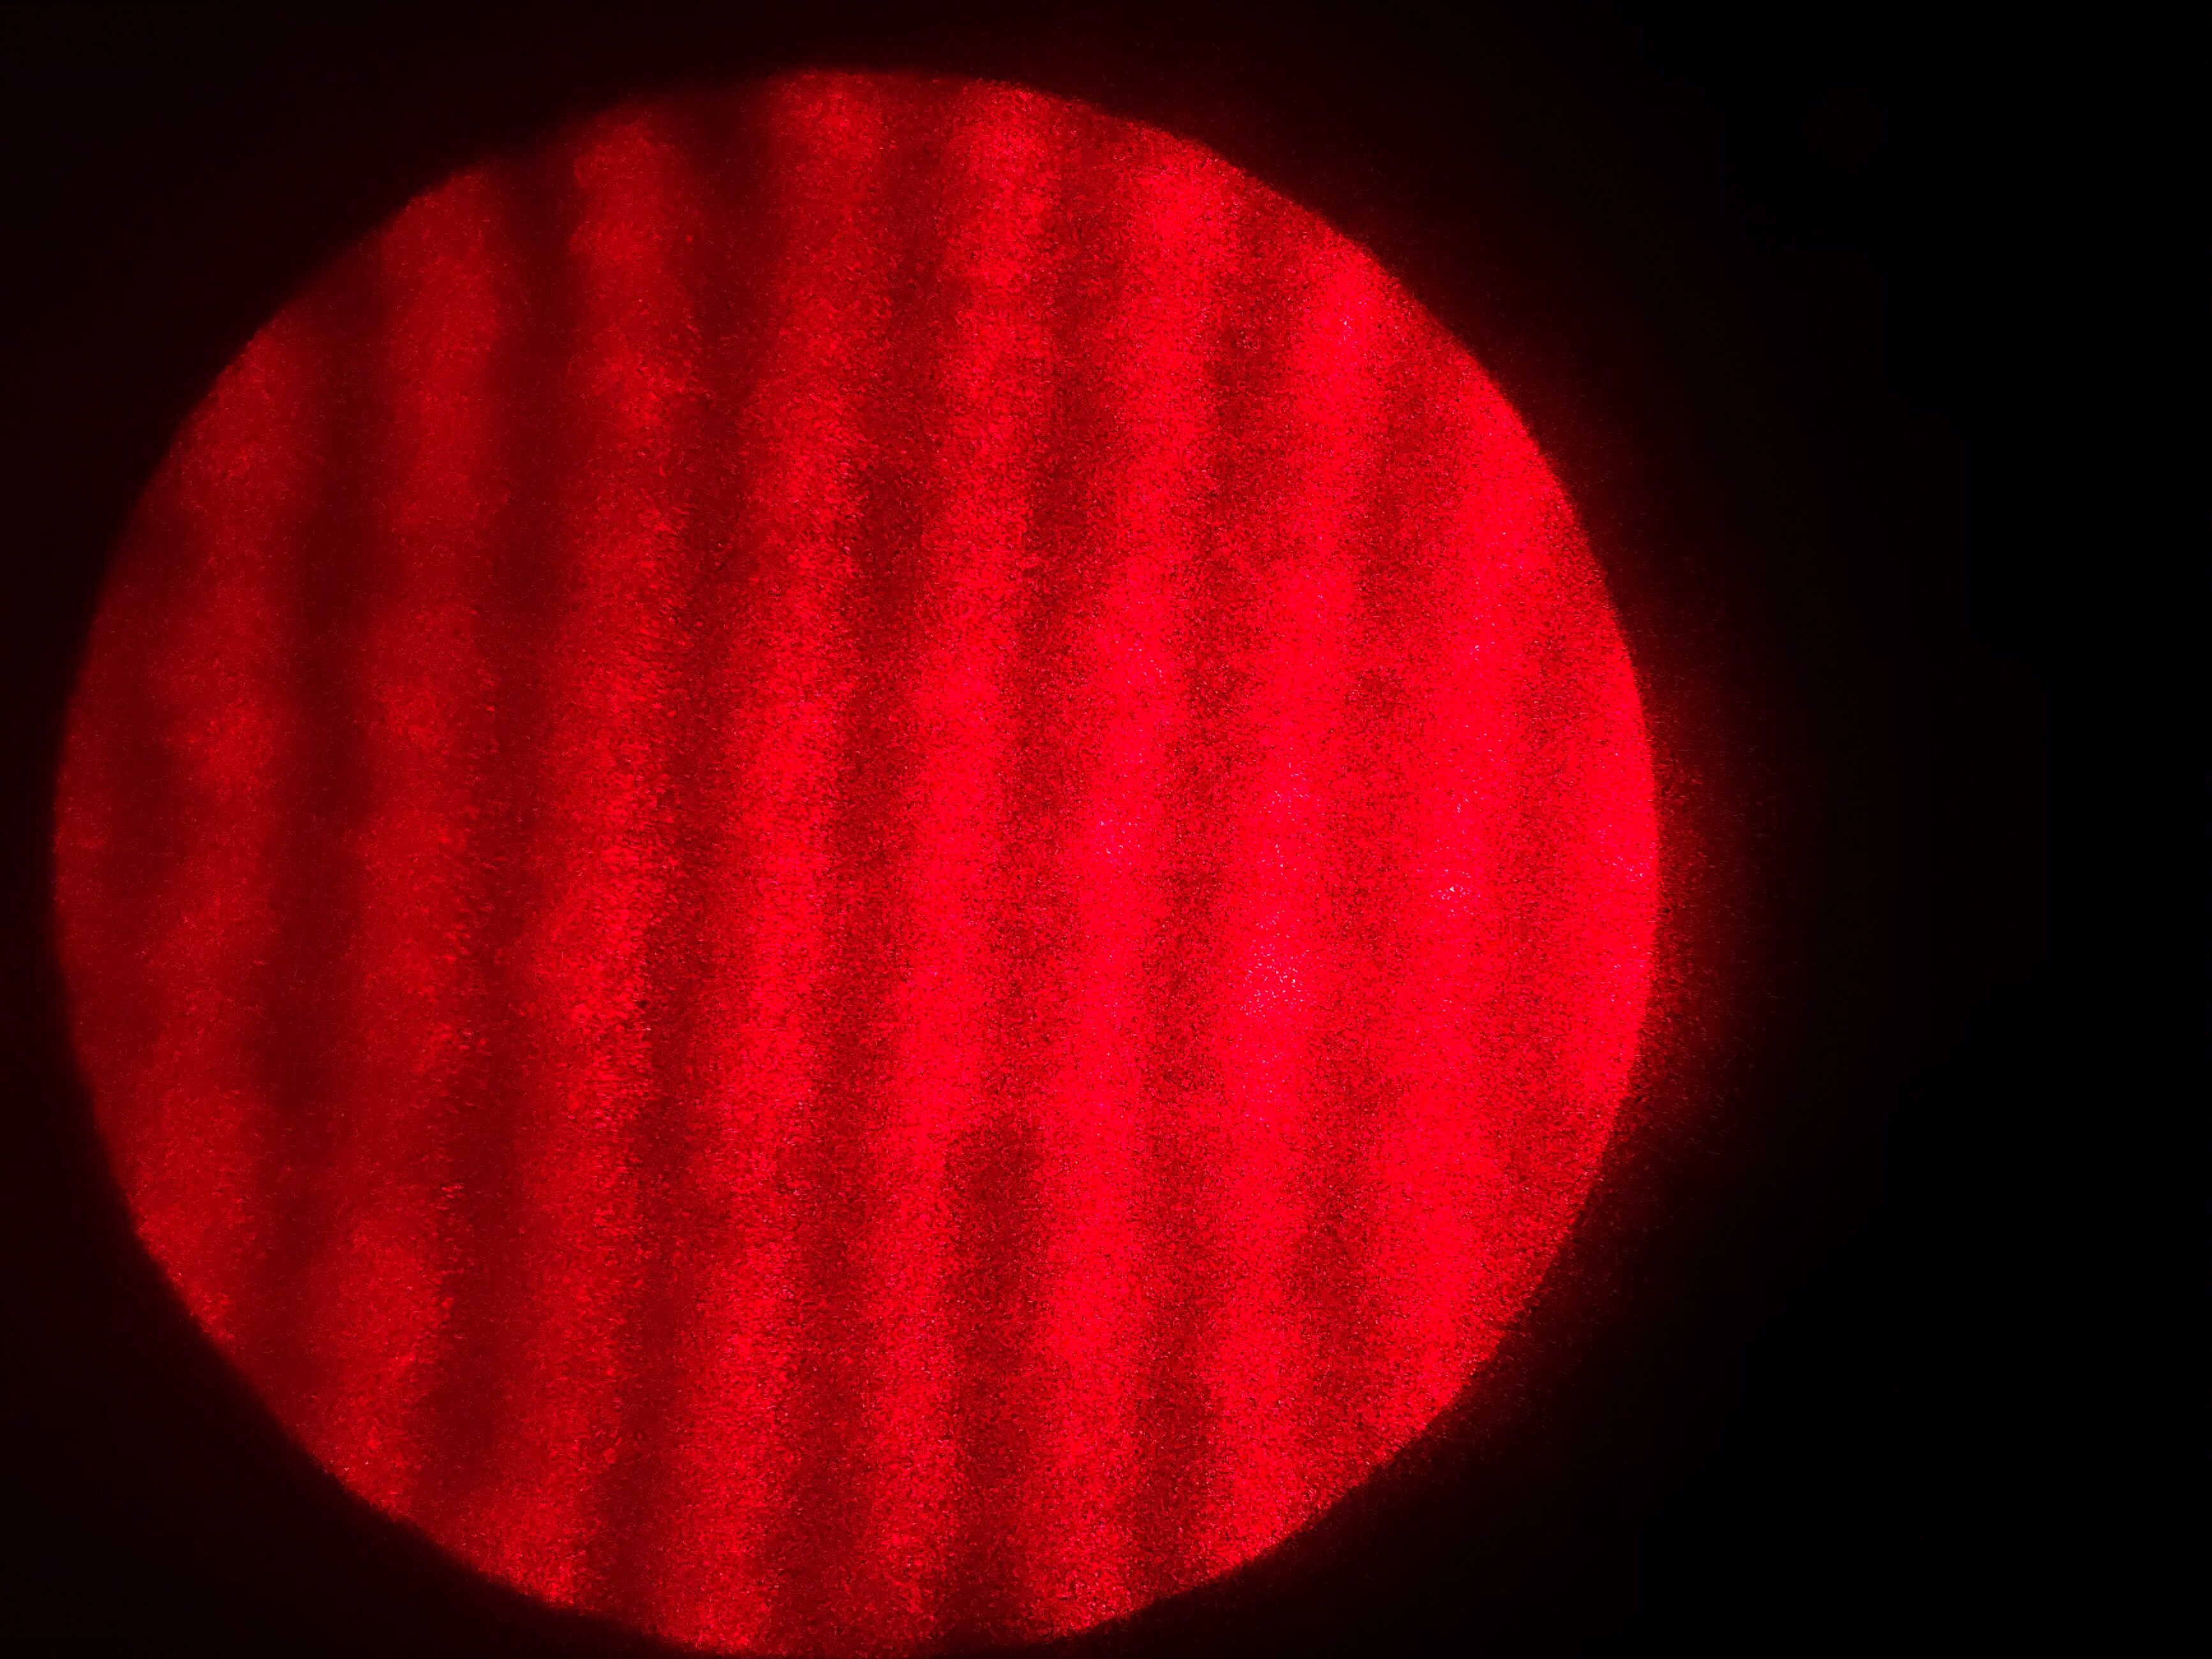
\includegraphics[width=0.45\textwidth]{一维-0级1级-显微镜.jpg}}
            \caption{通过0级、$\pm 1$级的衍射点}
        \end{figure*}

        此时能在光屏上看到条纹,但条纹明显没有全通过时的清晰。因为$\pm 1$级衍射点能提供光栅的基频信息,让条纹轮廓在像面上出现,
        但更高级的衍射条纹被遮挡掉了,因此无法提供全部的细节信息,所以条纹并不是非常清晰。

        
        \item [(4)] 除$\pm 1$外通过 \\
        \begin{table}[htb]
            \centering
            \begin{tabular}{|c|c|c|c|}
                \hline
                通过的点 & 起点位置$x/mm$ & 10个条纹后的位置$x'/mm$ & 条纹间距$d/mm$ \\
                \hline
                全部 & 31.090 & 33.748 & 0.2658 \\
                \hline
            \end{tabular}
            \caption{条纹间距测量结果}
        \end{table}
        \newpage
        \begin{figure*}[htb]
            \centering
            \subfigure[光屏上的像]{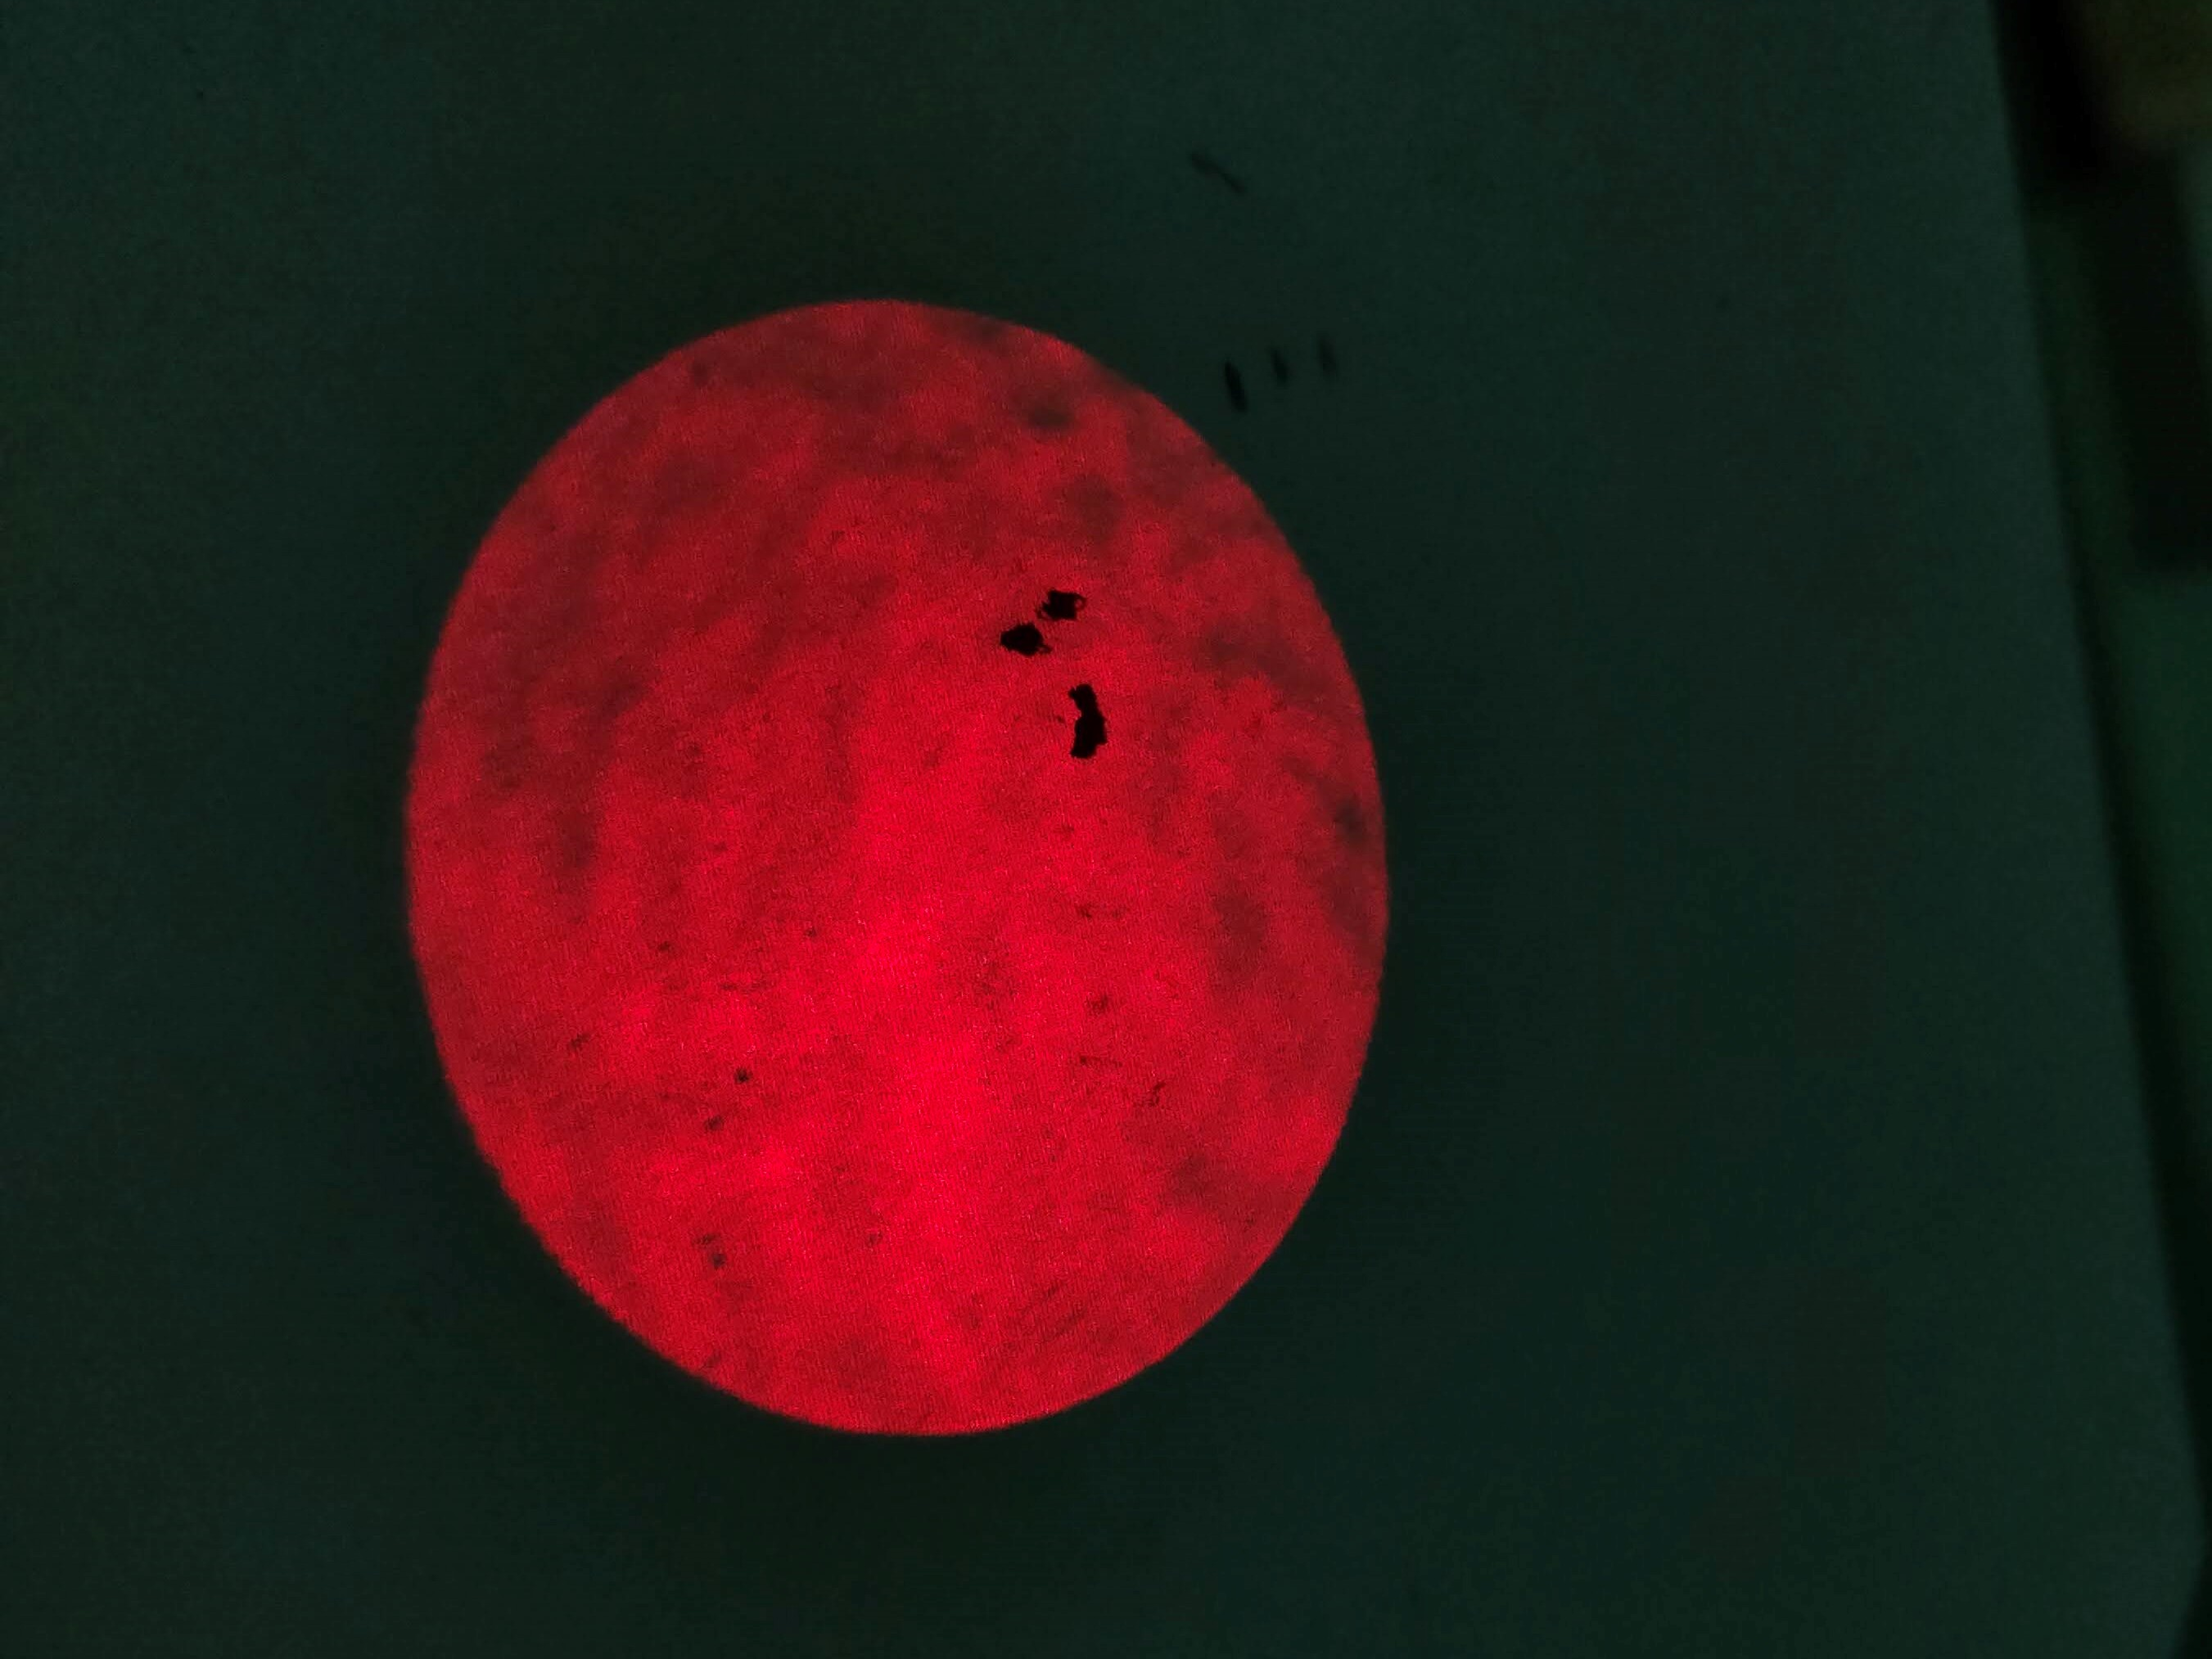
\includegraphics[width=0.45\textwidth]{一维-除1级外-屏.jpg}}
            \subfigure[显微镜中的像]{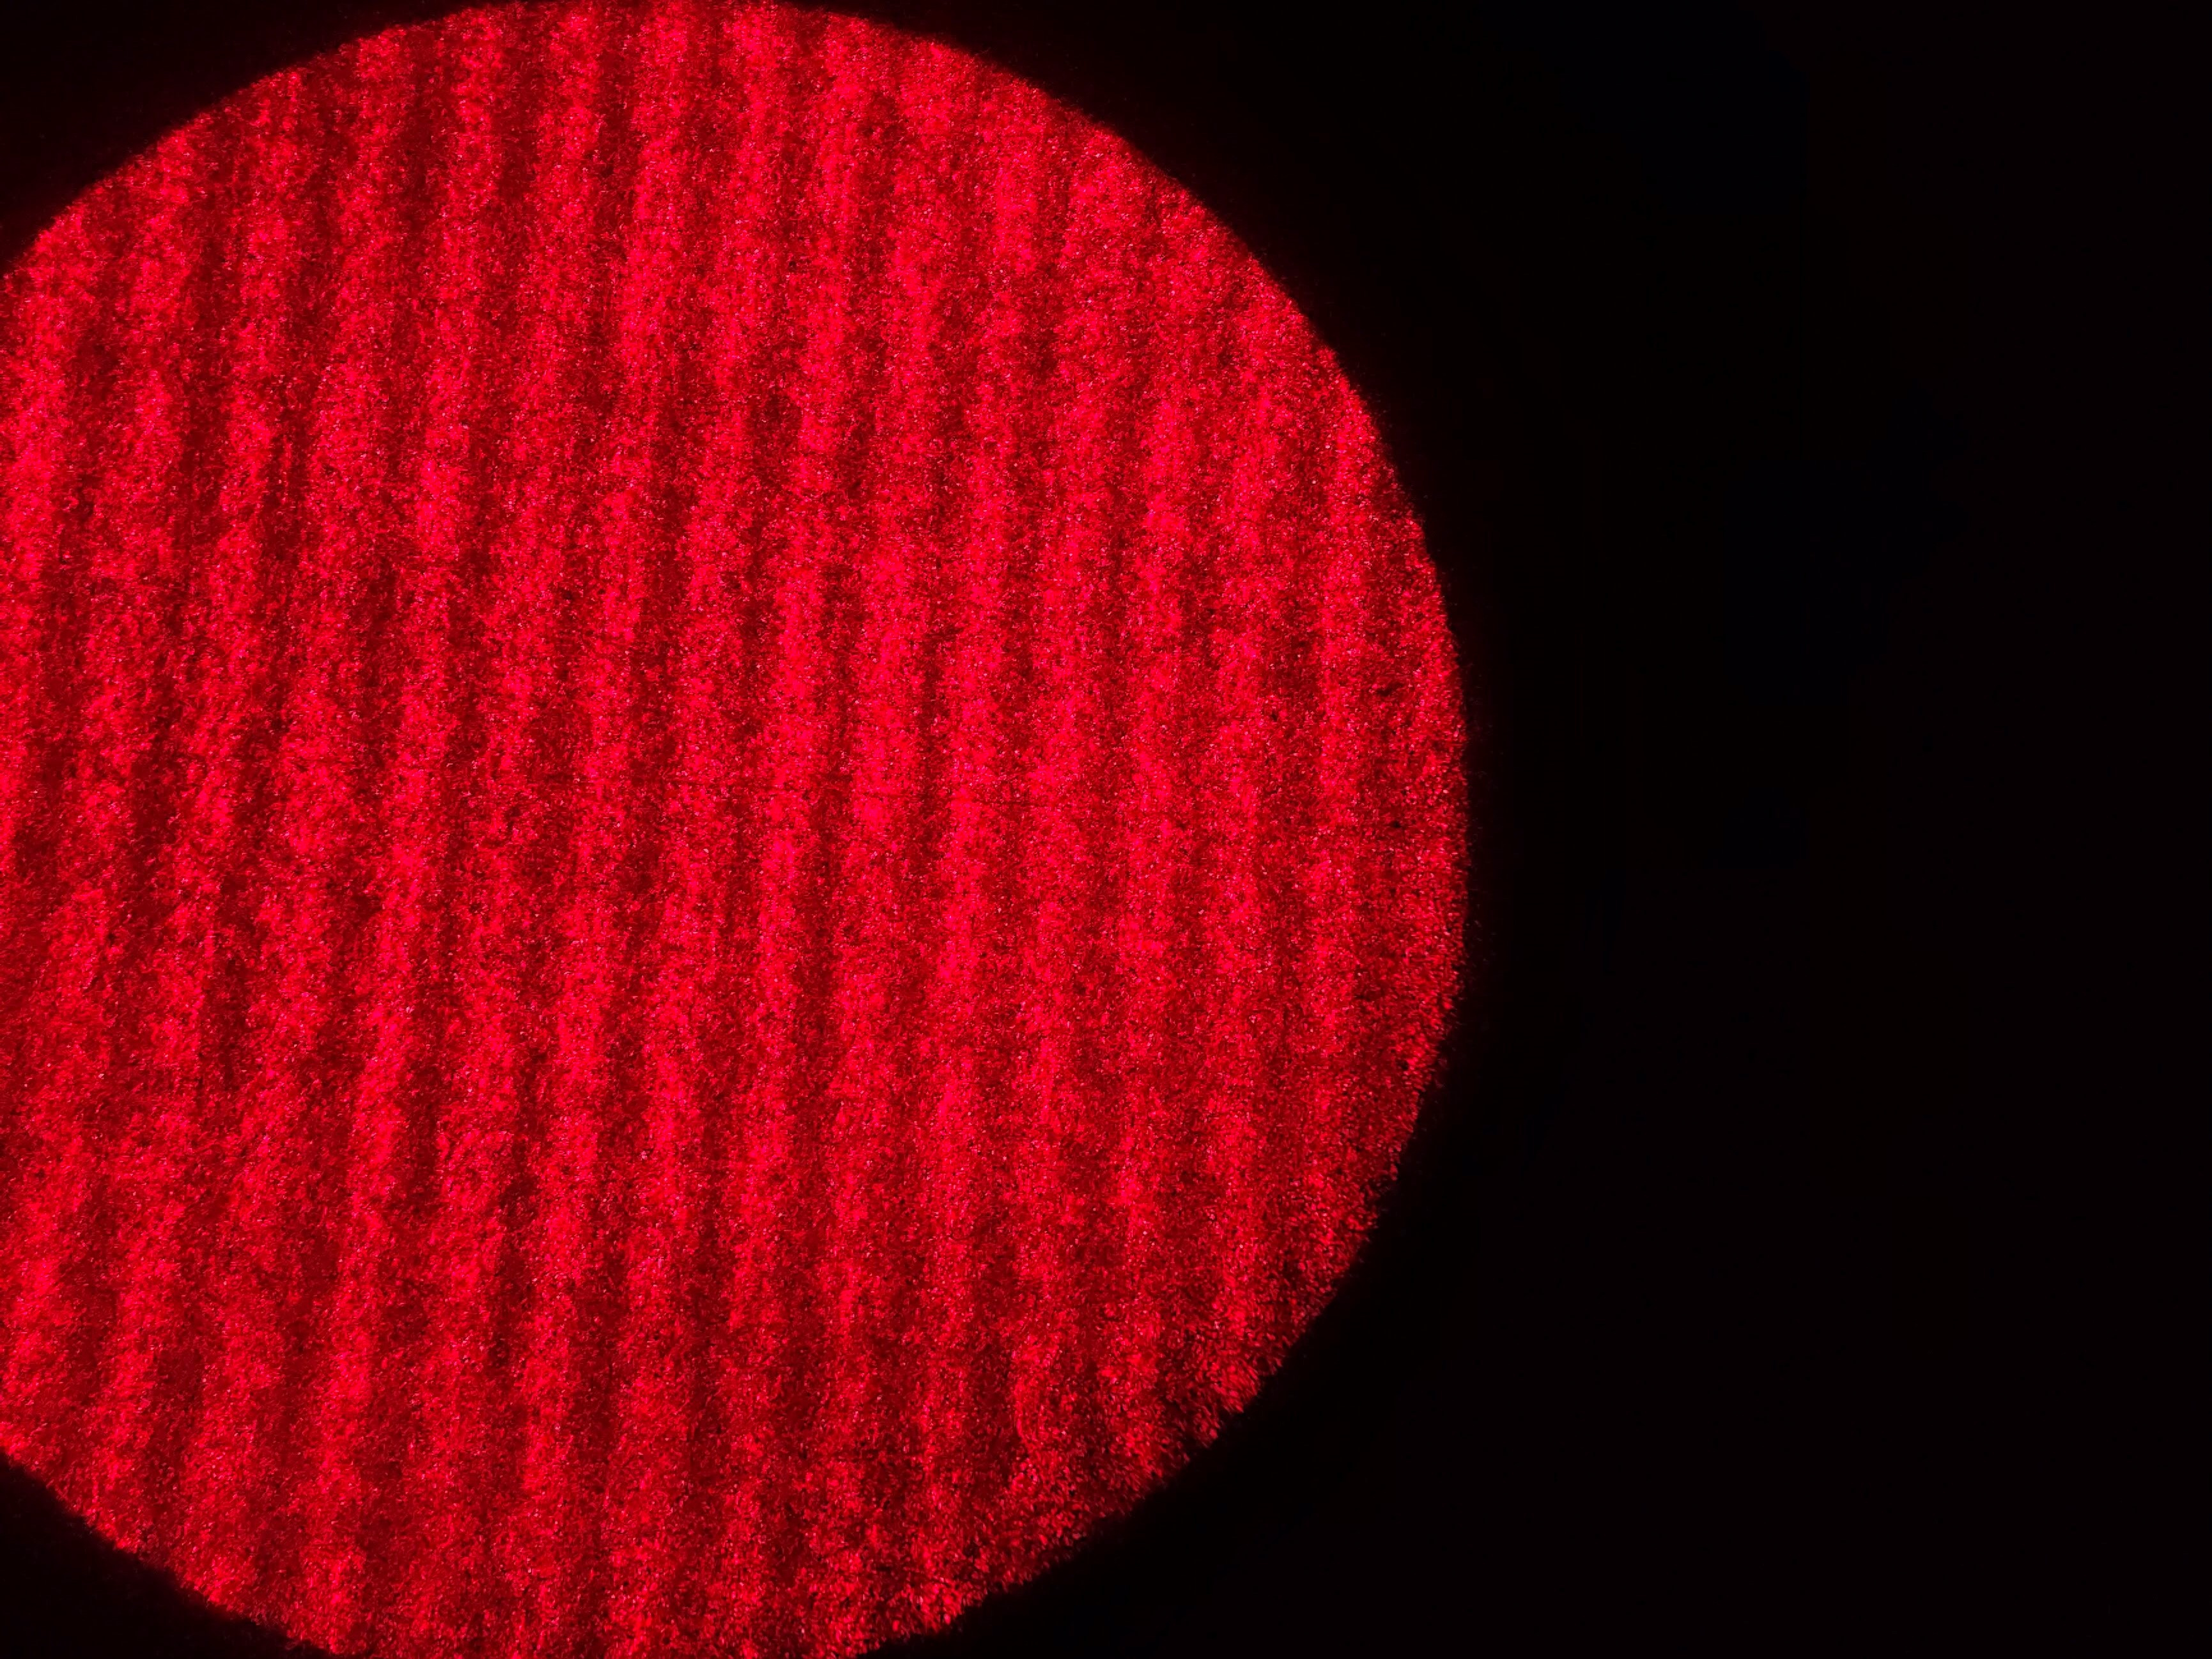
\includegraphics[width=0.45\textwidth]{一维-除1级外-显微镜.jpg}}
            \caption{通过除$\pm 1$级外}
        \end{figure*}

        光屏上和显微镜中能看到较为清晰的条纹,但可以观察到条纹变密。根据表6中条纹间距的测量结果,条纹间距变为了原来的一半。
        这是因为$\pm 1$级衍射点被挡掉,频谱中基频信号丢失,只剩下2倍频、3倍频……也就是说,原来的2倍频现在成为了“基频”,因此光栅成像
        的空间频率变为了原来的2倍,条纹间距变为了原来的一半。
        
        \item [(5)] 通过除0级外的衍射点 \\
        \begin{table}[htb]
            \centering
            \begin{tabular}{|c|c|c|c|}
                \hline
                通过的点 & 起点位置$x/mm$ & 10个条纹后的位置$x'/mm$ & 条纹间距$d/mm$ \\
                \hline
                全部 & 35.586 & 40.623 & 0.5037 \\
                \hline
            \end{tabular}
            \caption{条纹间距测量结果}
        \end{table}
        \begin{figure*}[h]
            \centering
            \subfigure[光屏上的像]{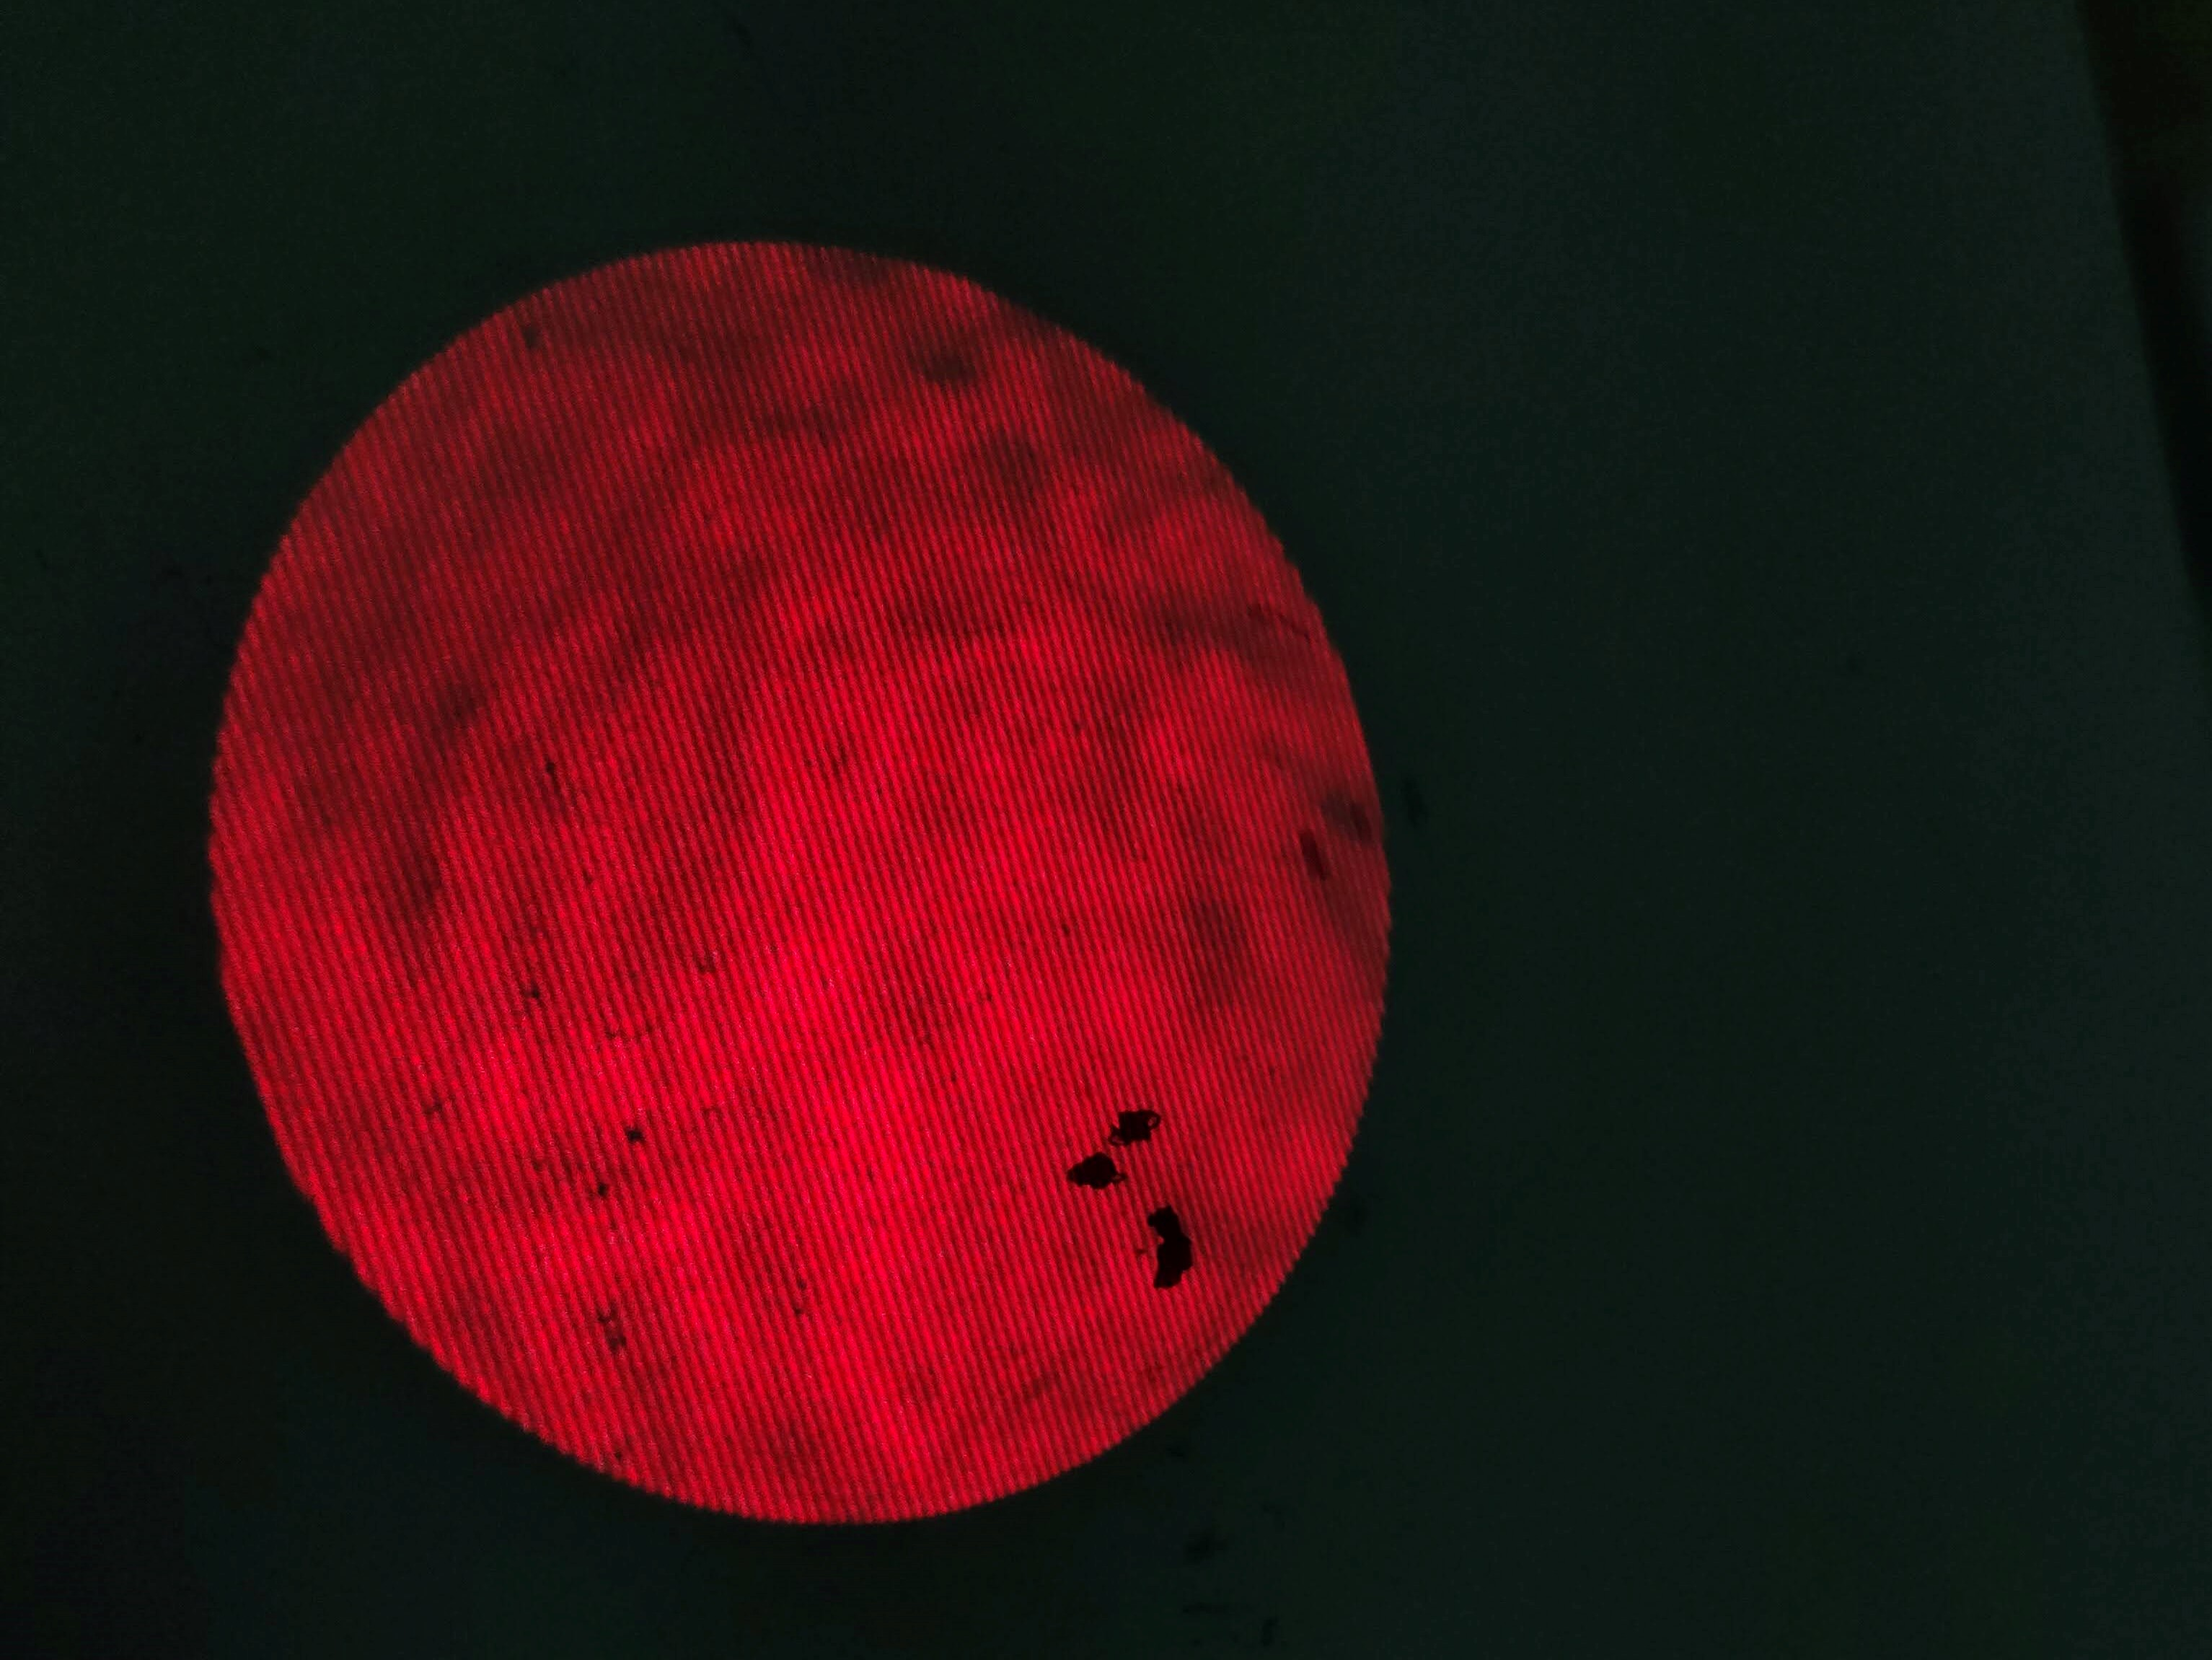
\includegraphics[width=0.45\textwidth]{一维-0级1级-屏.jpg}}
            \subfigure[显微镜中的像]{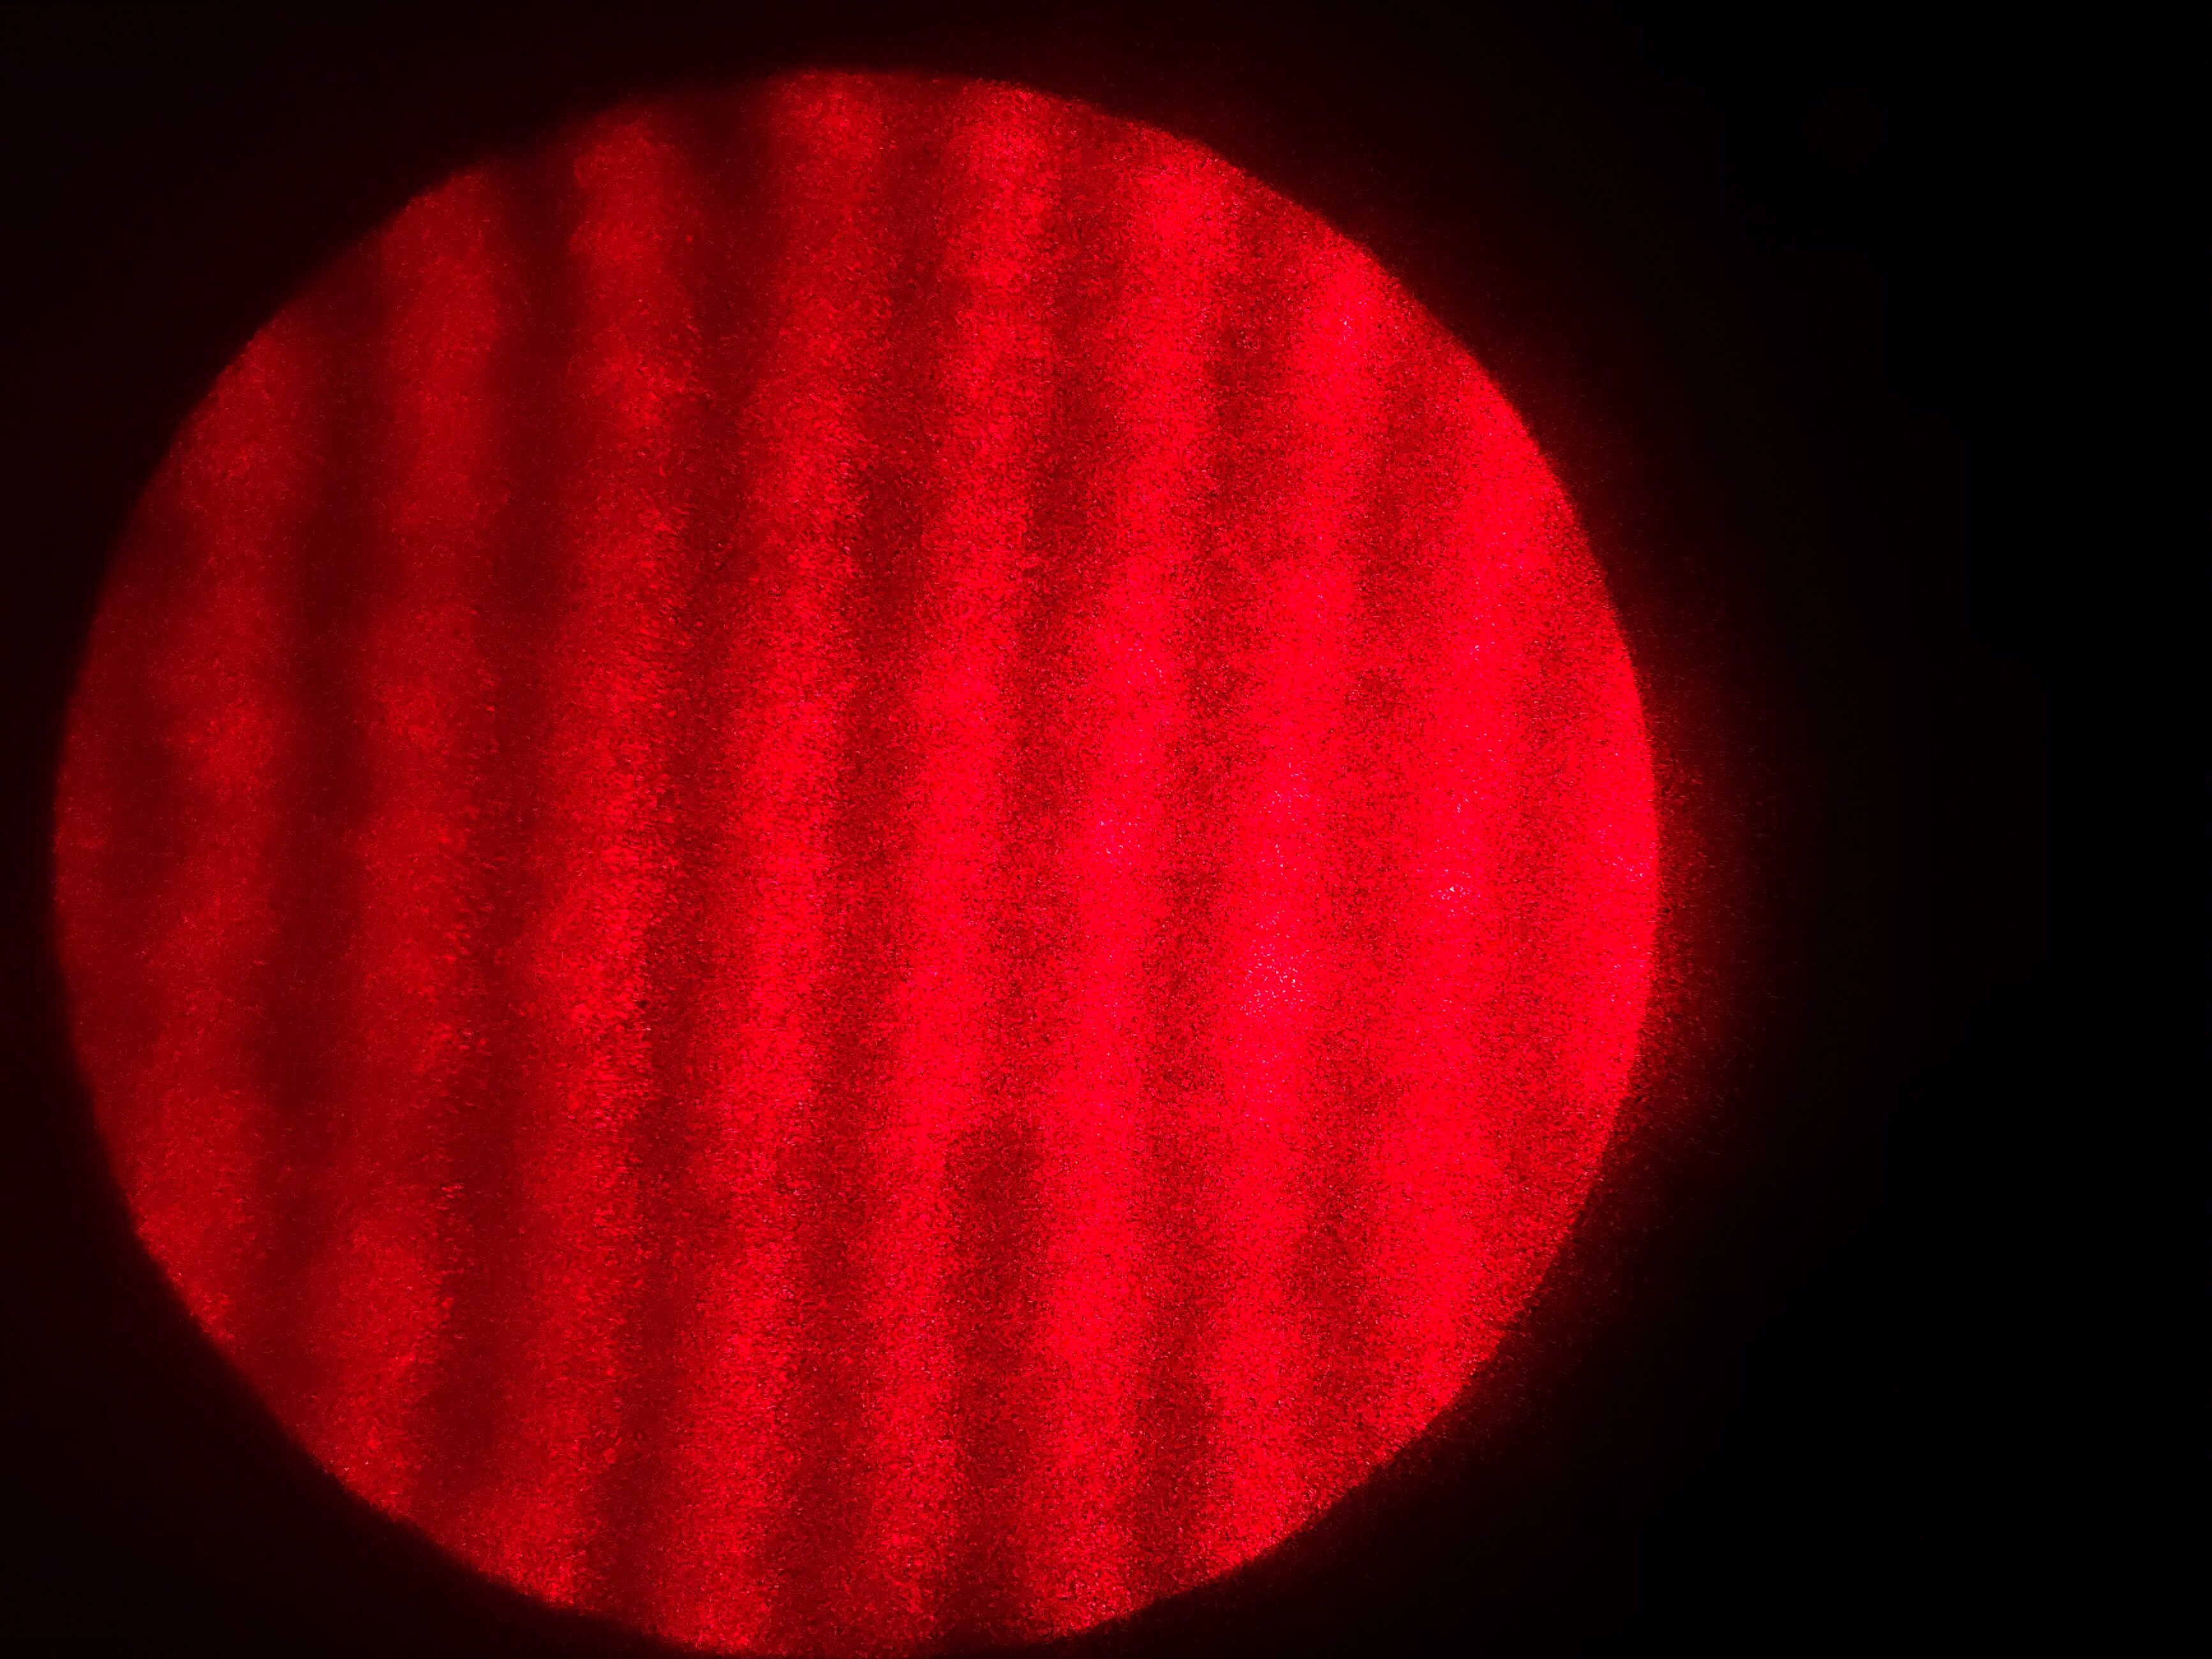
\includegraphics[width=0.45\textwidth]{一维-0级1级-显微镜.jpg}}
            \caption{通过除0级外}
        \end{figure*}

        光屏和显微镜中能看到较为清晰的条纹,条纹间距也没有明显变化,但从显微镜中观察,条纹的明暗对比下降了,也就是说,
        亮条纹和暗条纹之间的亮度差异减小了。这是因为0级衍射点能提供一个均匀的背景,当其被滤除,亮条纹就不再那么亮了。
    \end{enumerate}

    \subsection{二维光栅}
    \subsubsection{网格间距测量}
    将一维光栅换成二维光栅,在频谱边上可以二维离散的光点阵,像面上的成像情况如图6所示,可以看到网格状的条纹。
    条纹间距的测量结果如表8所示。
    \begin{figure*}[h]
        \centering
        \subfigure[光屏上的像]{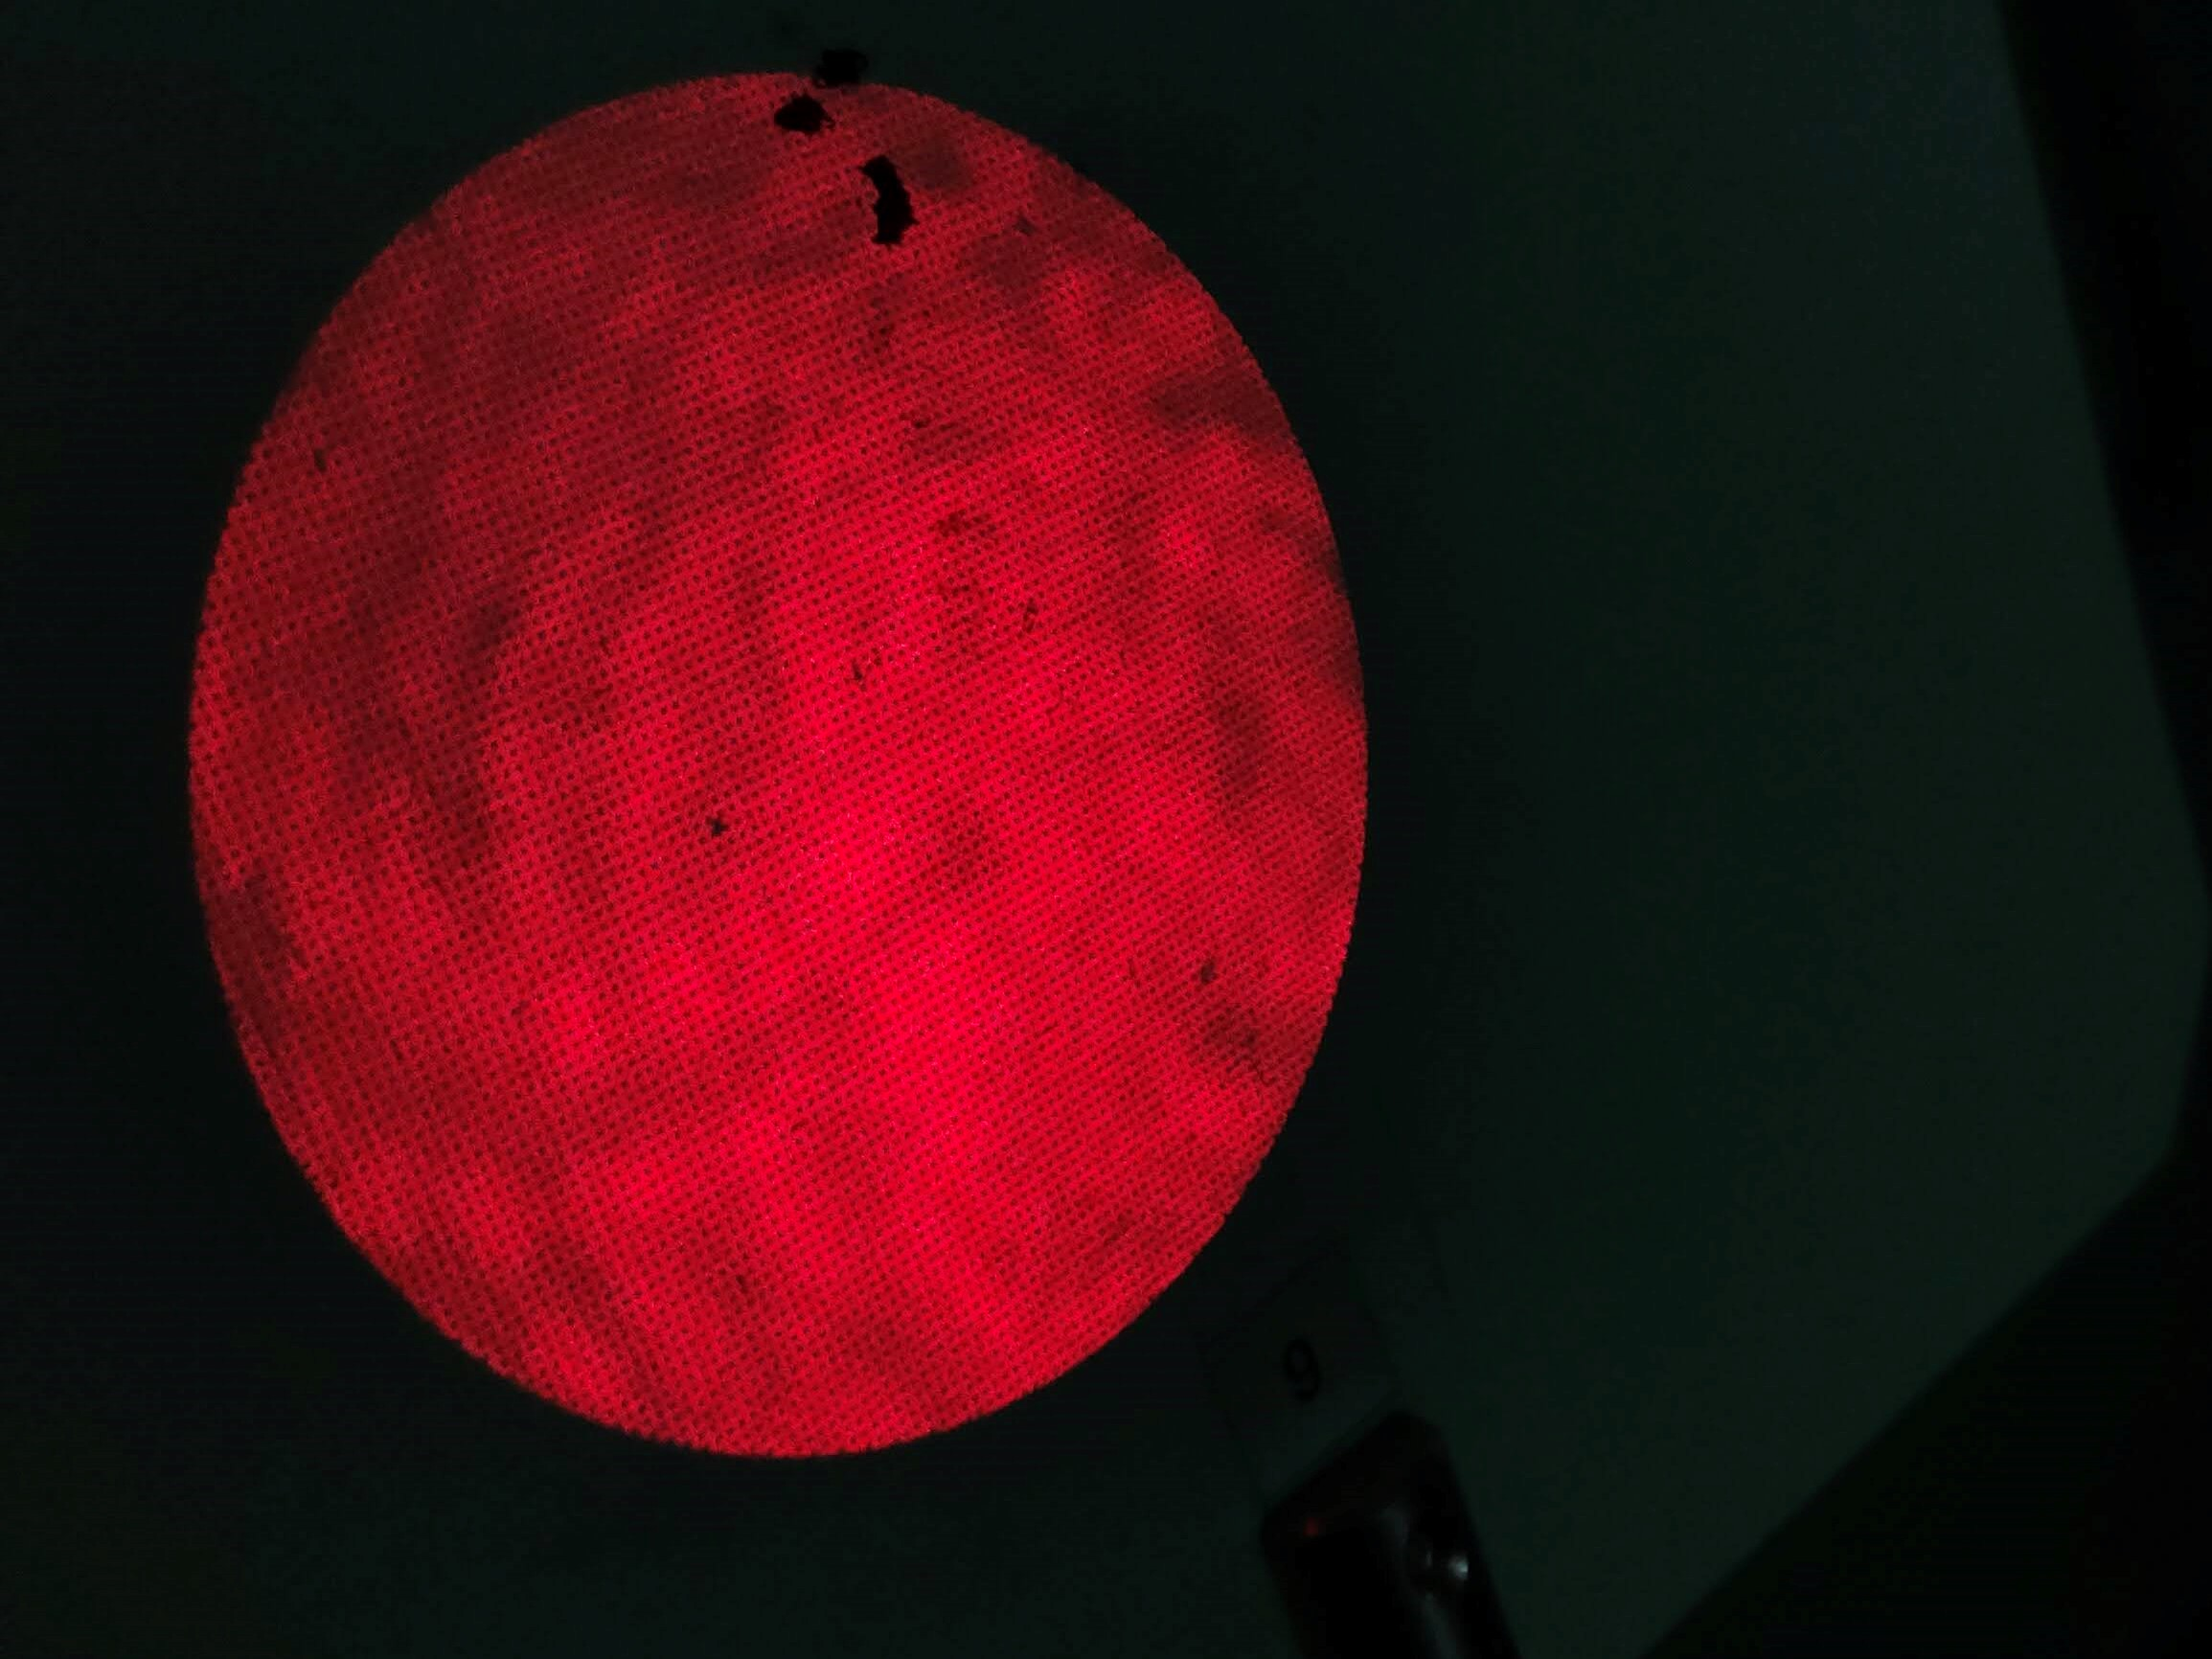
\includegraphics[width=0.45\textwidth]{二维-全通过-屏.jpg}}
        \subfigure[显微镜中的像]{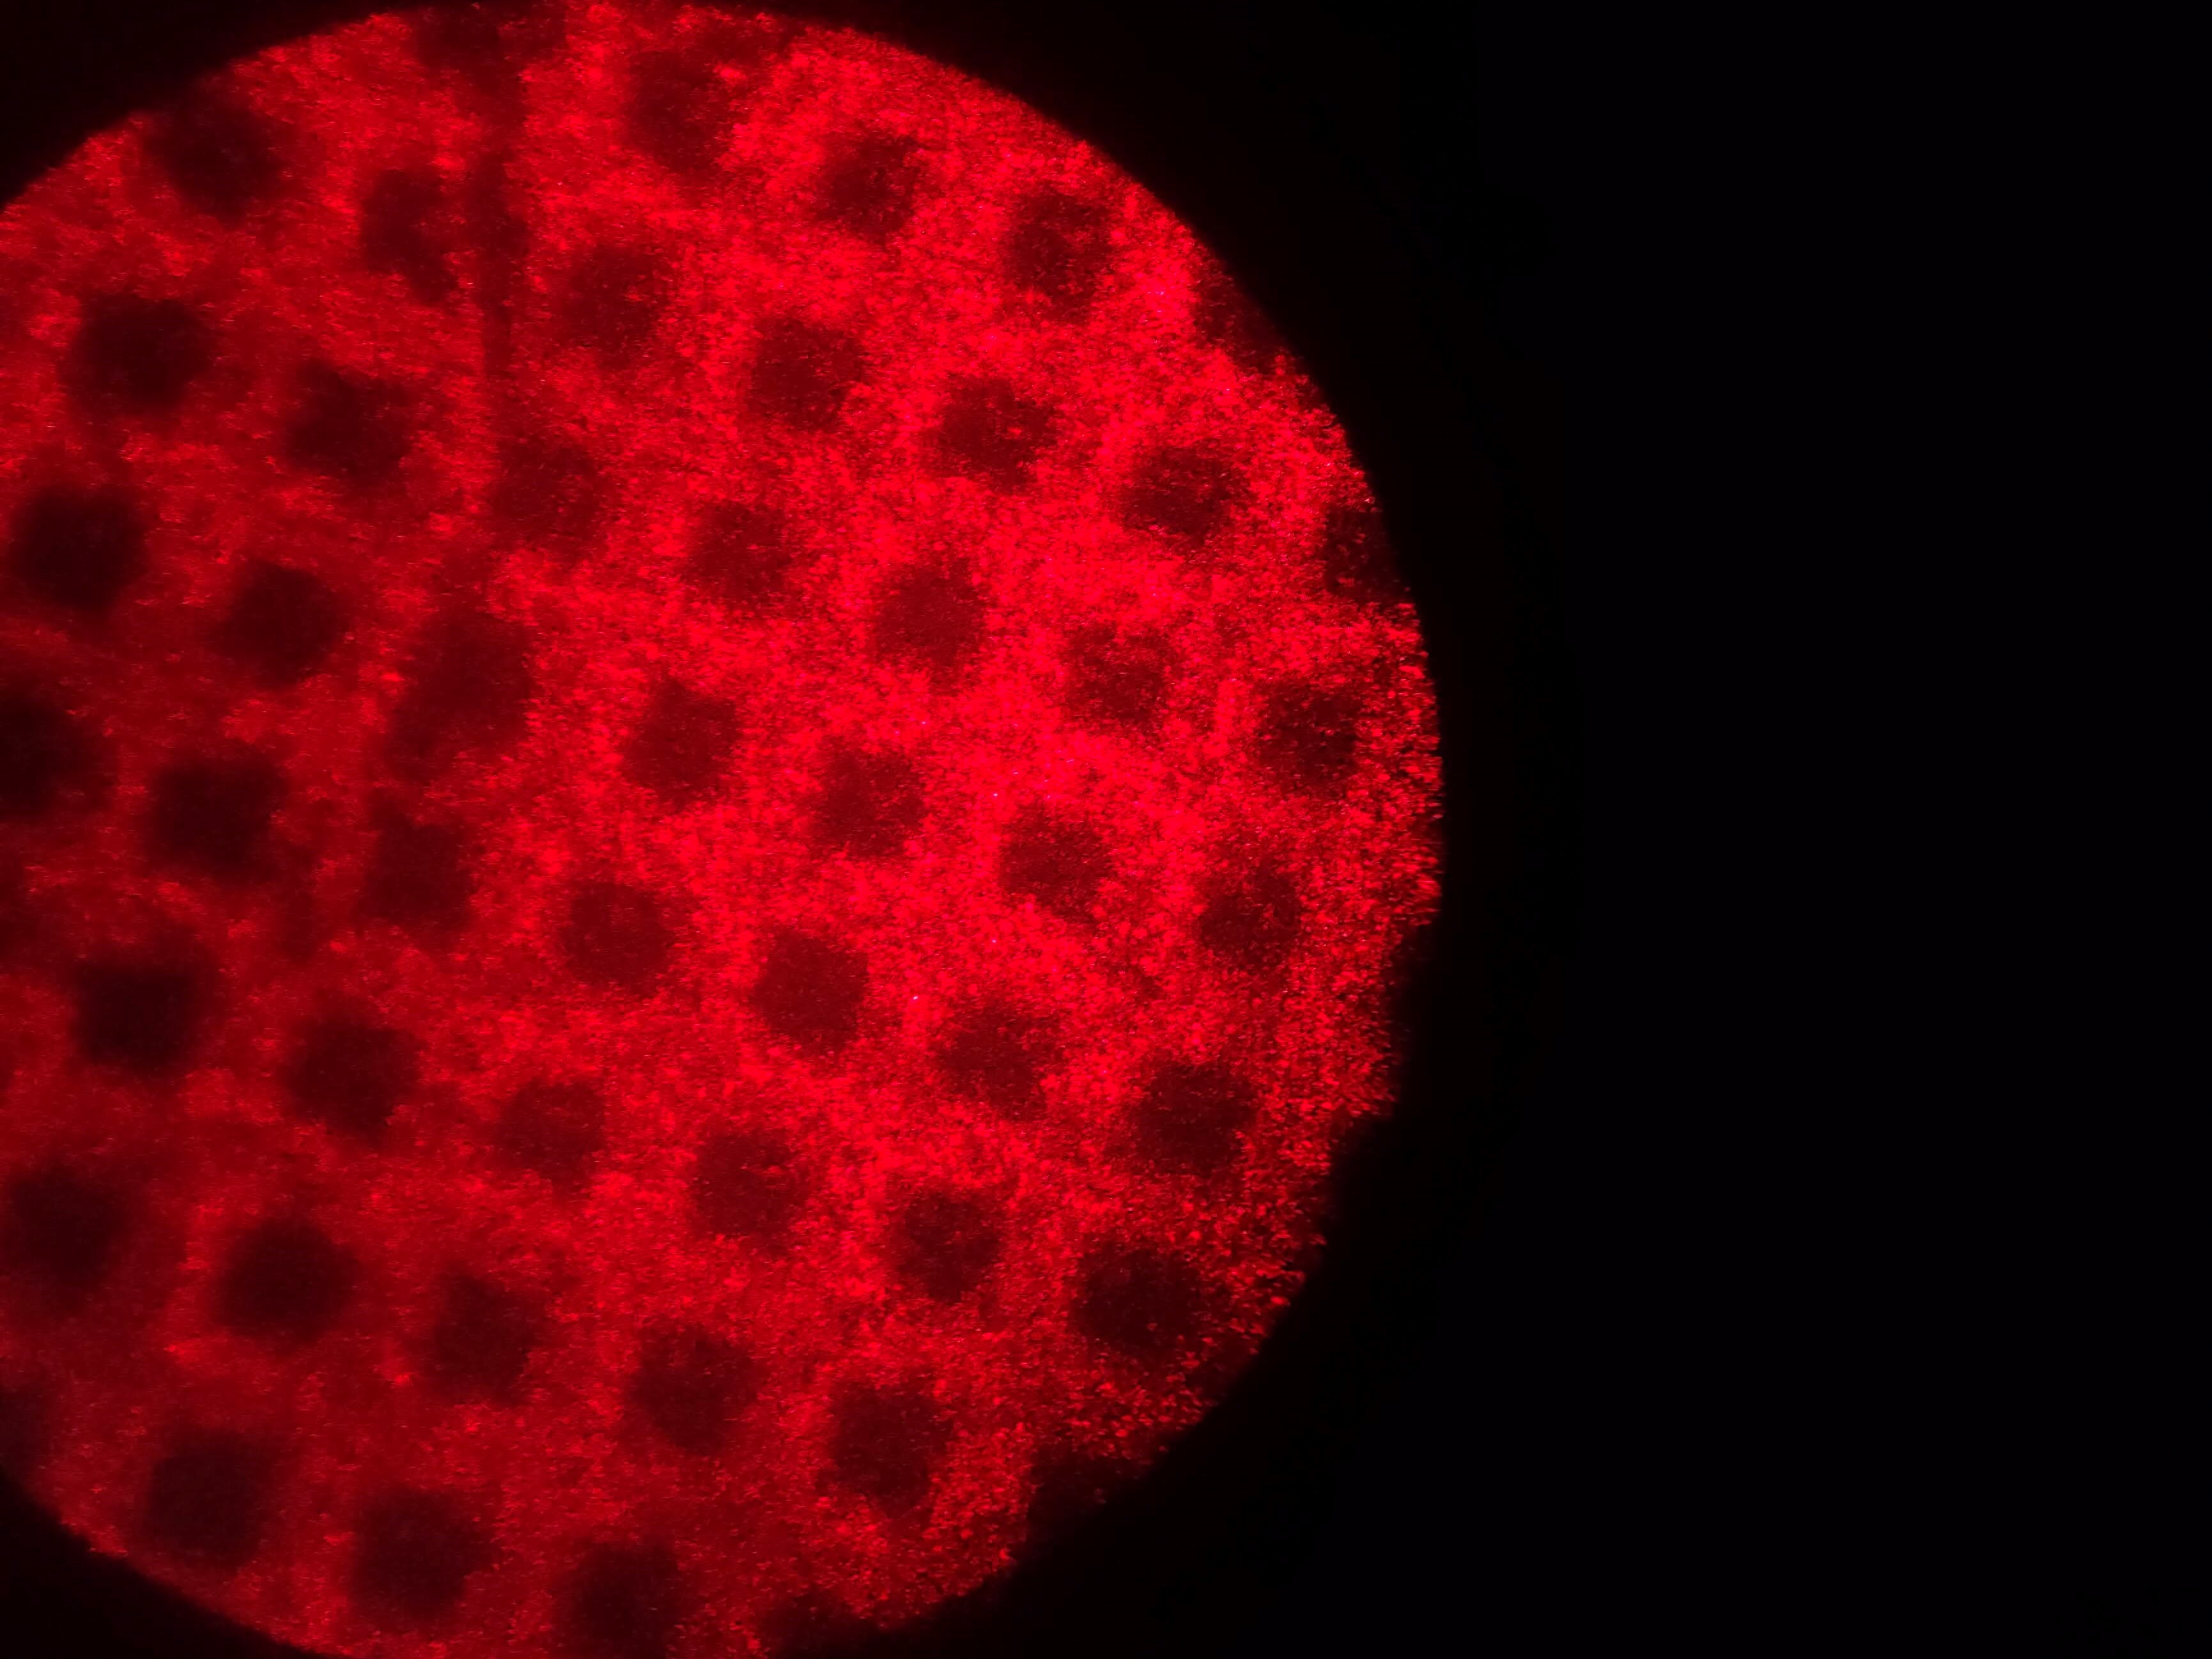
\includegraphics[width=0.45\textwidth]{二维-全通过-显微镜.jpg}}
        \caption{二维正交光栅成像}
    \end{figure*}
    \begin{table}[h]
        \centering
        \begin{tabular}{ |c|c|c|c| }
            \hline
            通过的点 & 起点位置$x/mm$ & 11个条纹后的位置$x'/mm$ & 条纹间距$d/mm$ \\
            \hline
            全部 & 33.899 & 40.083 & 0.5622 \\
            \hline
        \end{tabular}
        \caption{条纹间距测量结果}
    \end{table}

    \subsubsection{空间滤波实验}
    在频谱面上放上不同的圆孔或狭缝光阑进行滤波,观察像面上的条纹和条纹间距。

    \begin{enumerate}
        \item [(1)] 小孔 \\
        光屏上只能看到一片均匀的红色光斑,无法看见条纹。因为小孔光阑只允许中央的0级衍射点通过,无法提供任何细节信息。
        \newpage
        \begin{figure*}[h]
            \centering
            \subfigure{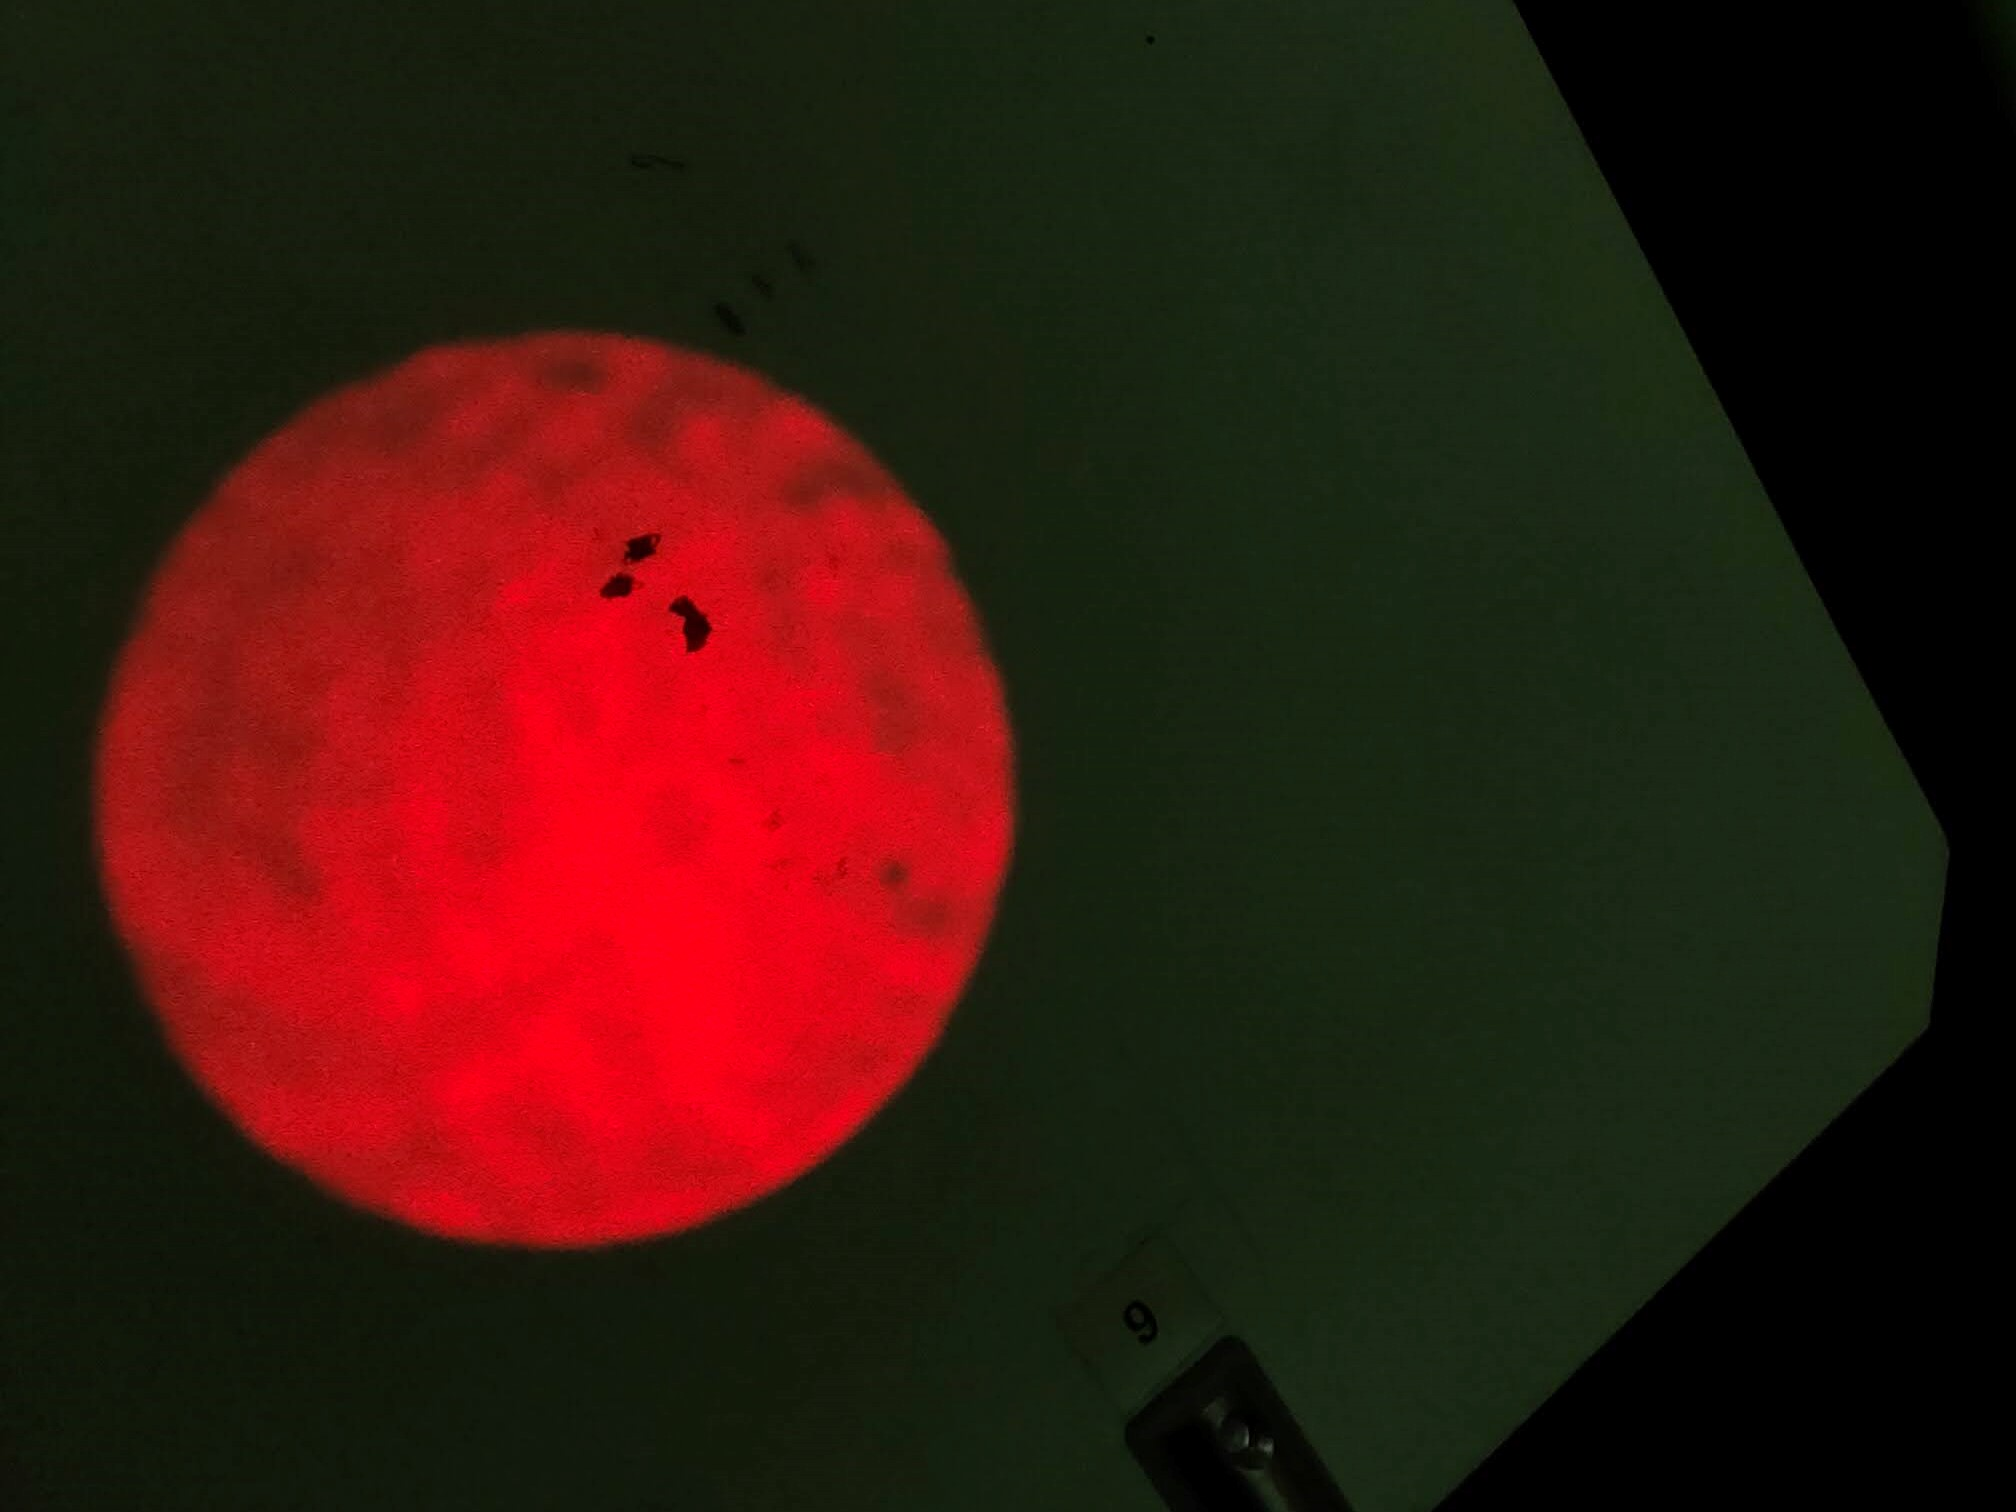
\includegraphics[width=0.45\textwidth]{二维-孔-屏.jpg}}
            \caption{小孔光阑}
        \end{figure*}
    
        \item [(2)] 纵狭缝 \\
        在频谱面上放上纵狭缝,只允许竖直方向的衍射光斑通过,在光屏上可以看到水平方向的条纹。这相当于滤除了竖直方向的光栅信息,只保留水平方向的。
        由于条纹沿竖直方向交替而显微镜只能水平方向移动,故无法测量条纹间距。
        \begin{figure*}[h]
            \centering
            \subfigure[光屏上的像]{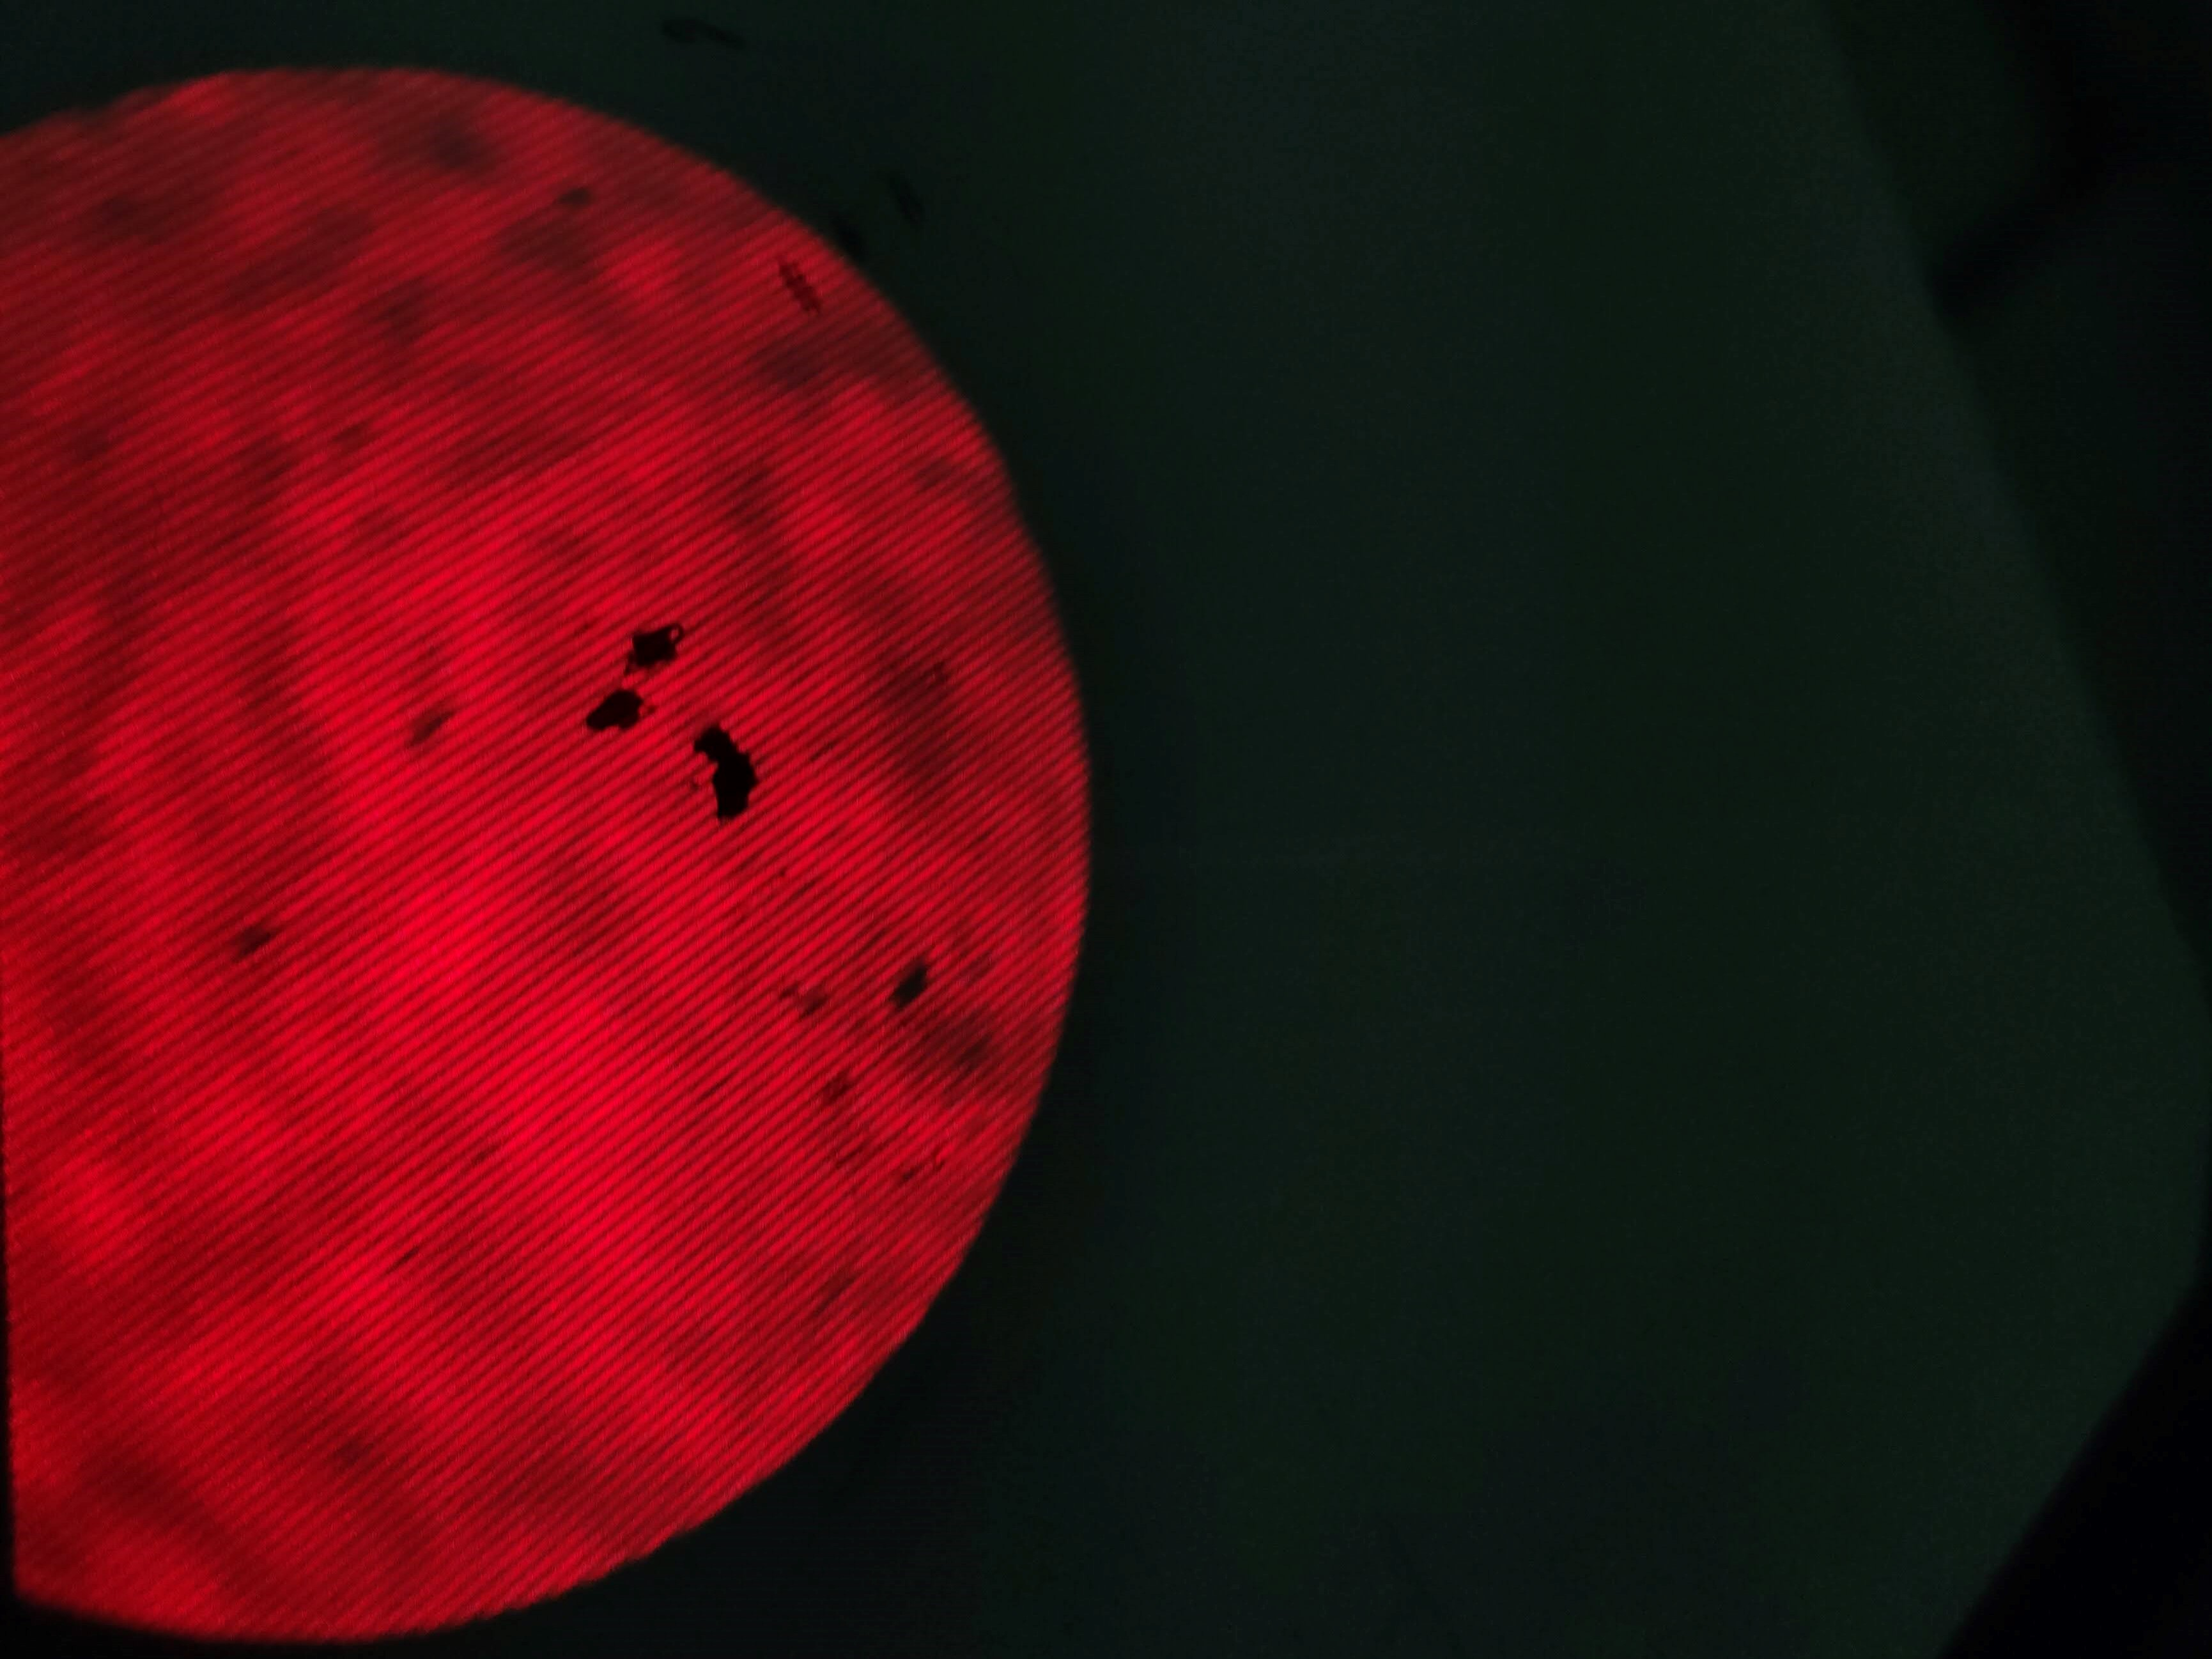
\includegraphics[width=0.45\textwidth]{二维-纵狭缝-屏.jpg}}
            \subfigure[显微镜中的像]{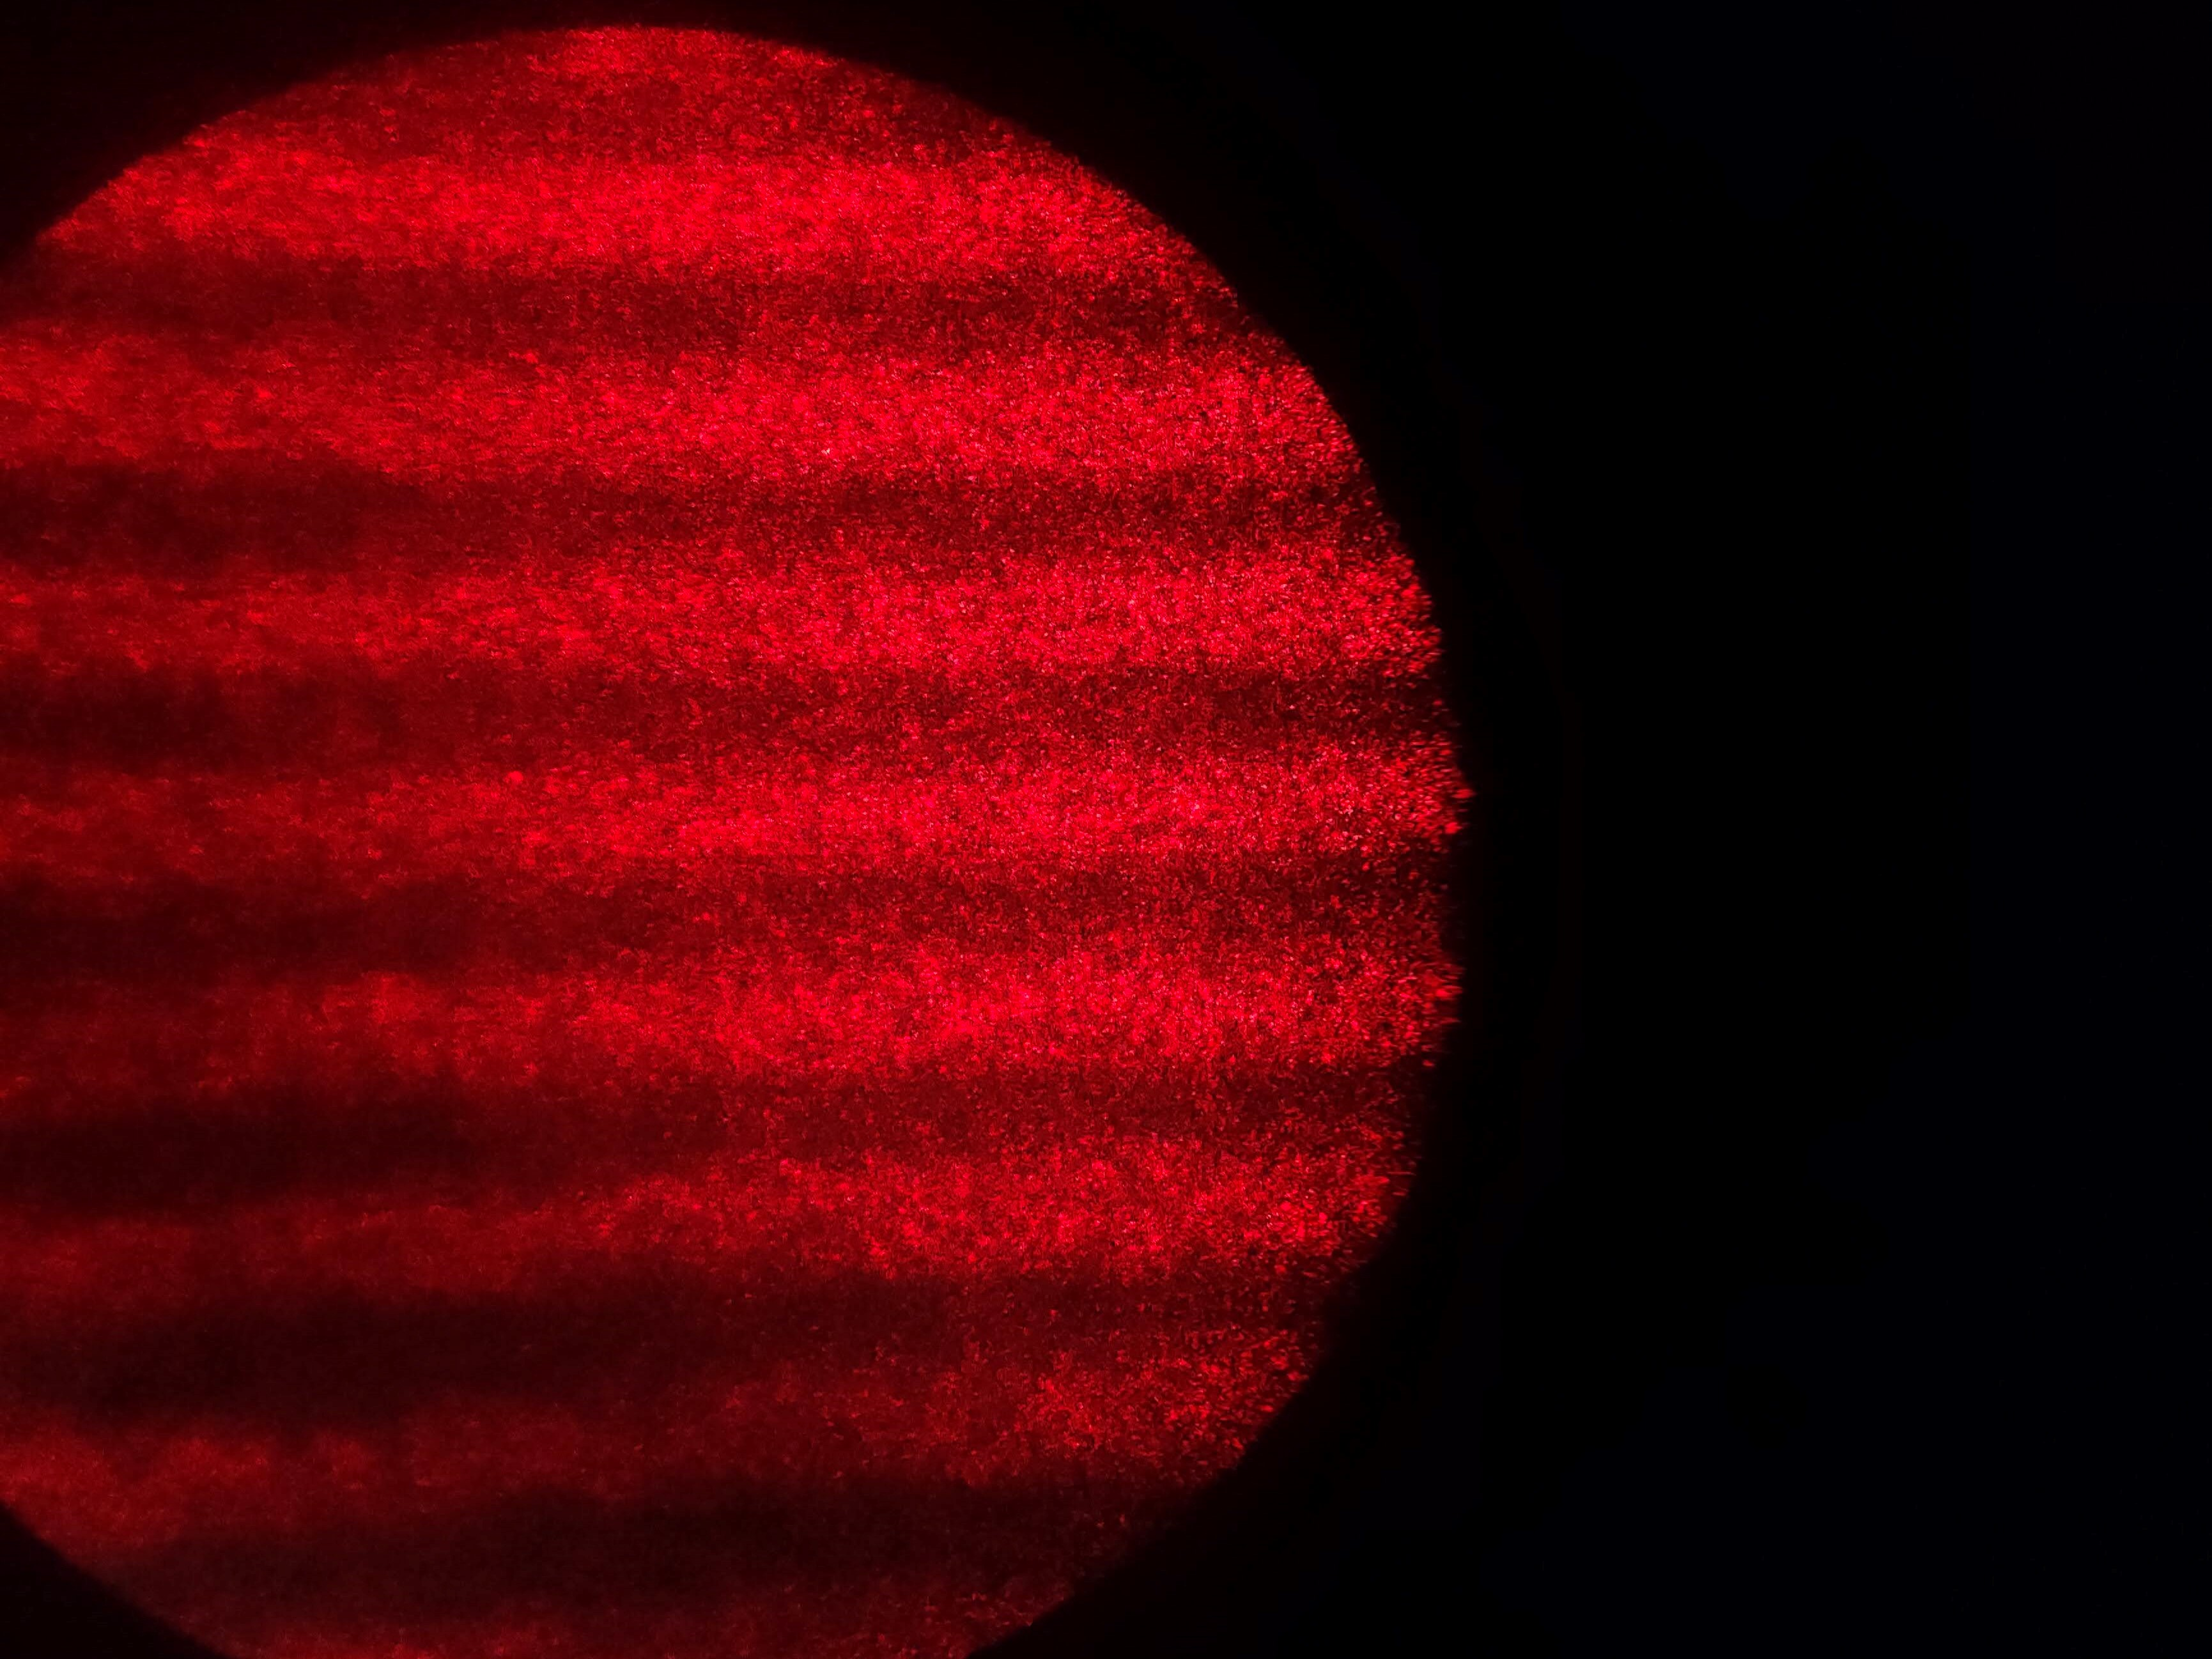
\includegraphics[width=0.45\textwidth]{二维-纵狭缝-显微镜.jpg}}
            \caption{纵狭缝光阑}
        \end{figure*}

        \item [(3)] 横狭缝\\
        在频谱面上放上横狭缝,只允许水平方向的衍射光斑通过,在光屏上可以看到竖直方向的条纹。这相当于滤除了水平方向光栅的信息,保留了竖直方向的光栅。
        根据表9所示的条纹间距测量结果,条纹间距与全通过时的二维光栅的条纹间距大致相同,因为此时看到的就是二维正交光栅的沿的水平分量。
        \newpage
        \begin{figure*}[h]
            \centering
            \subfigure[光屏上的像]{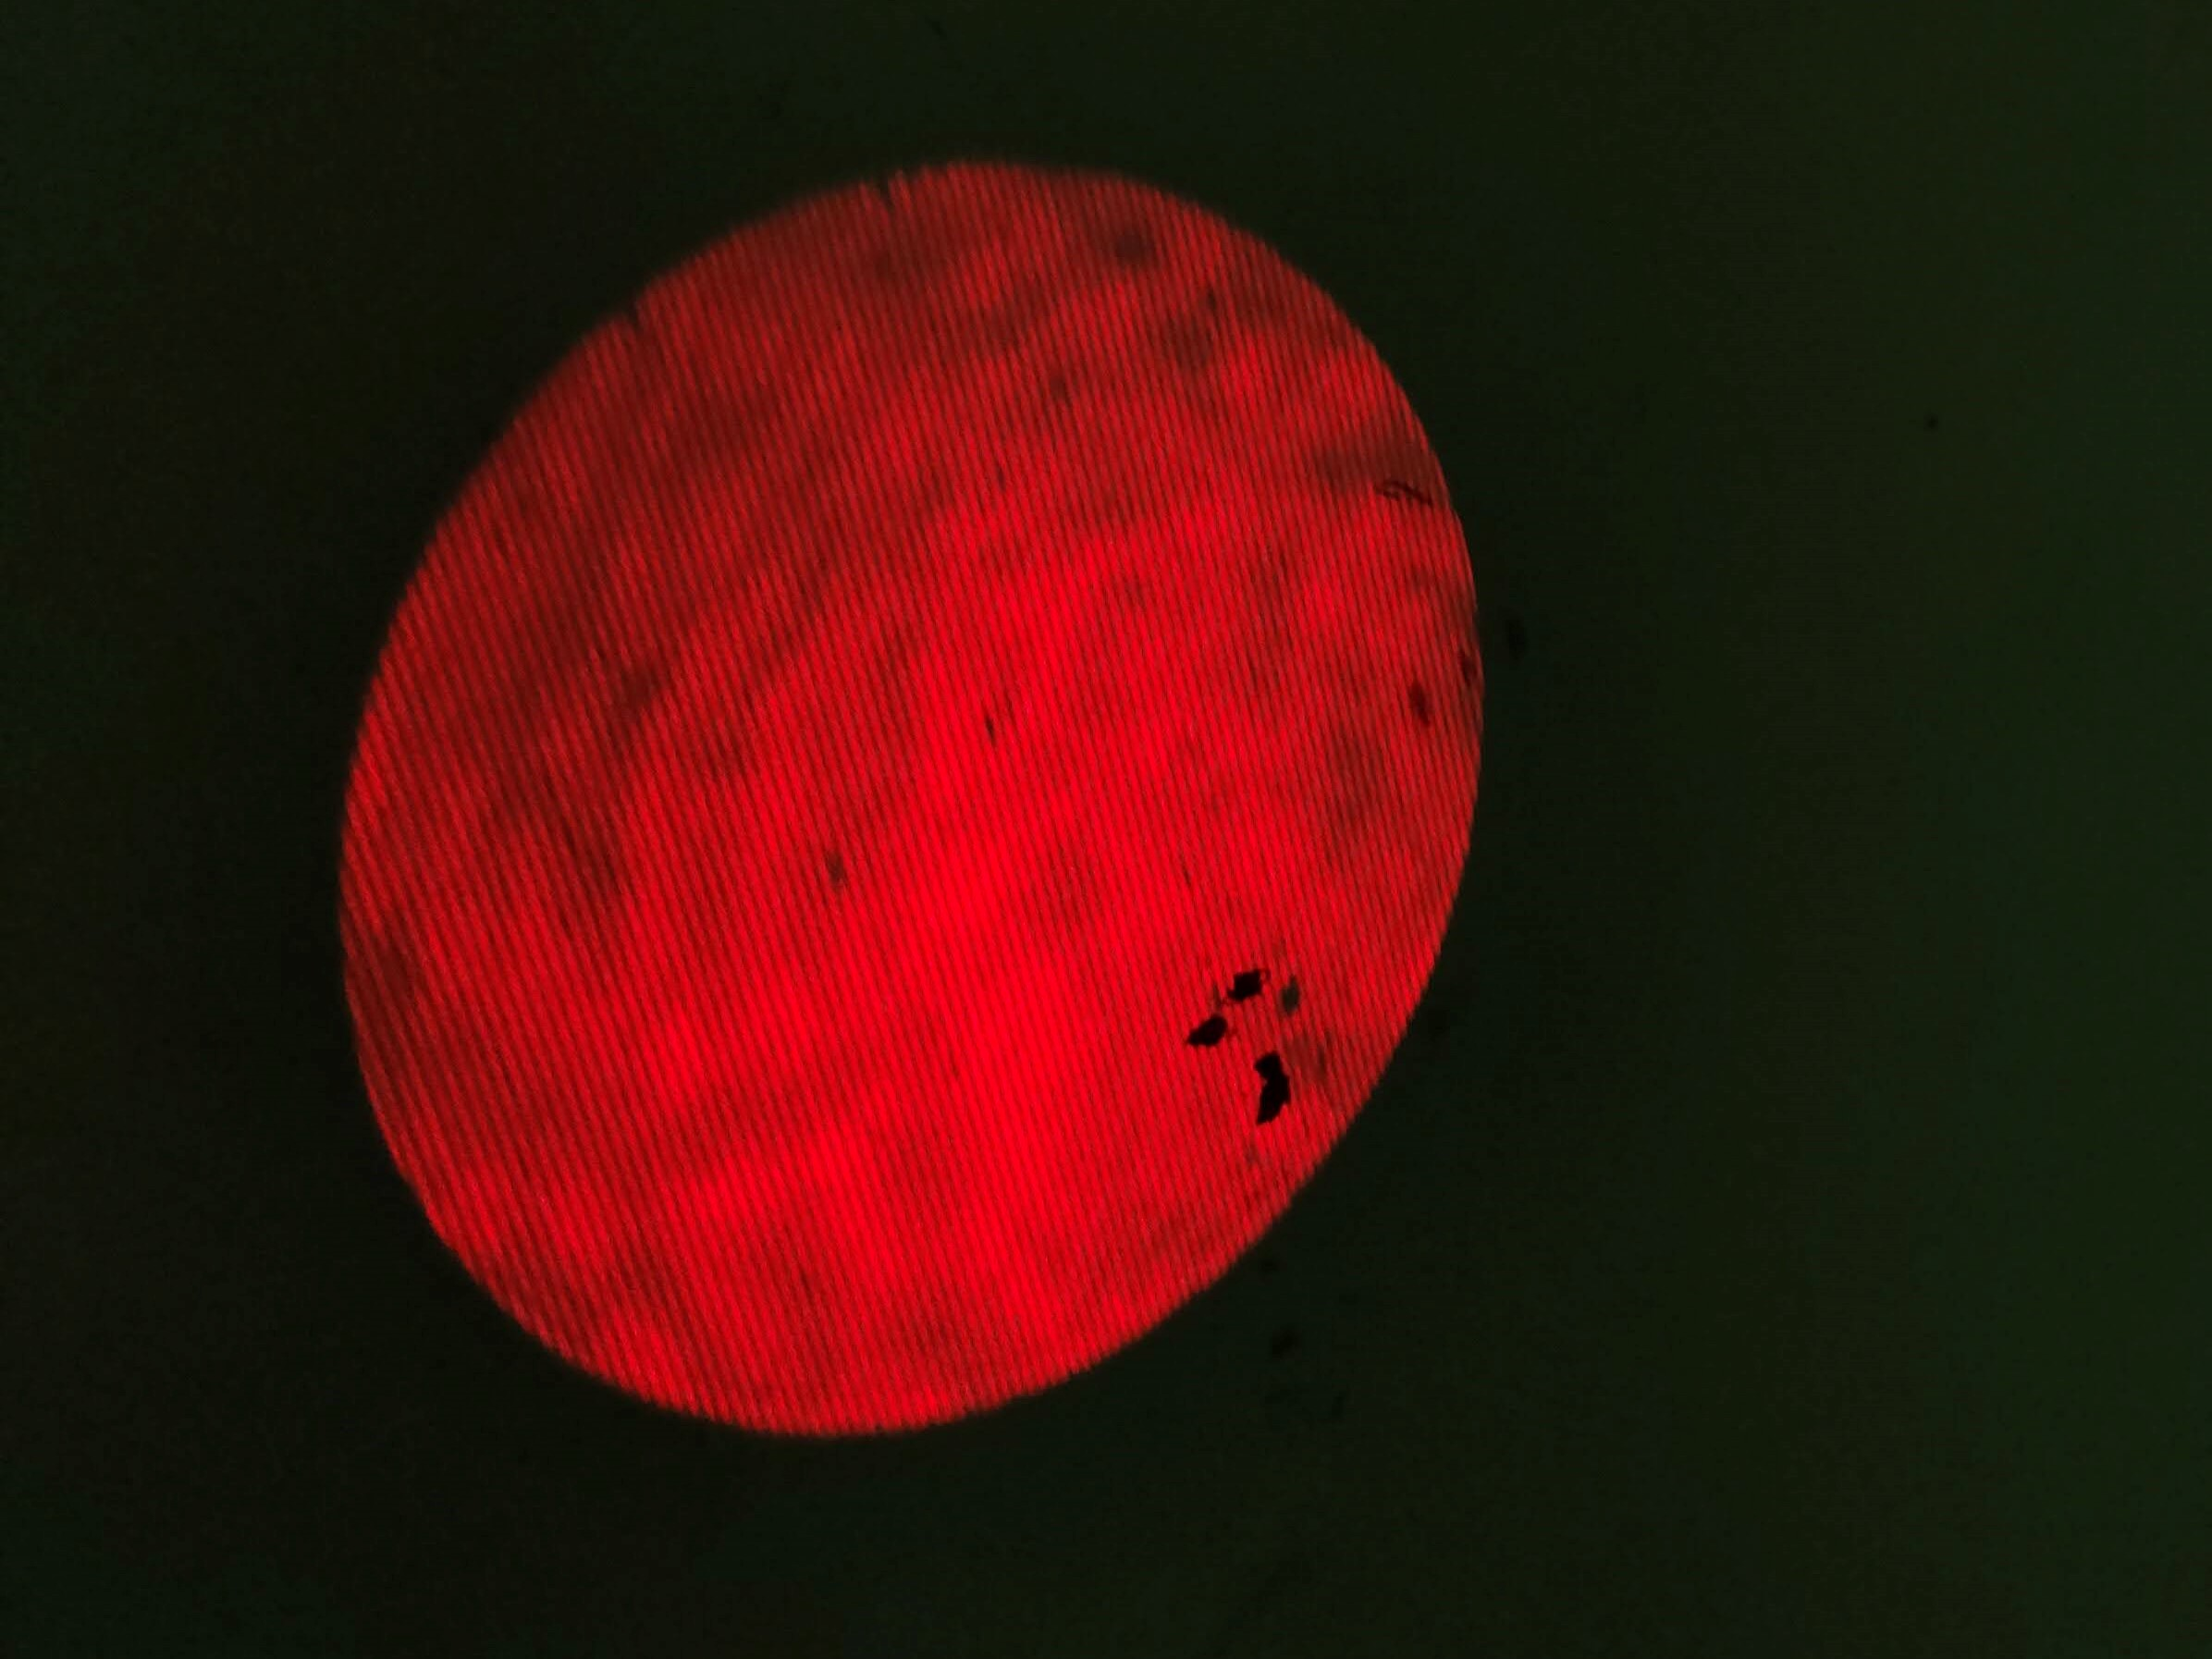
\includegraphics[width=0.45\textwidth]{二维-横狭缝-屏.jpg}}
            \subfigure[显微镜中的像]{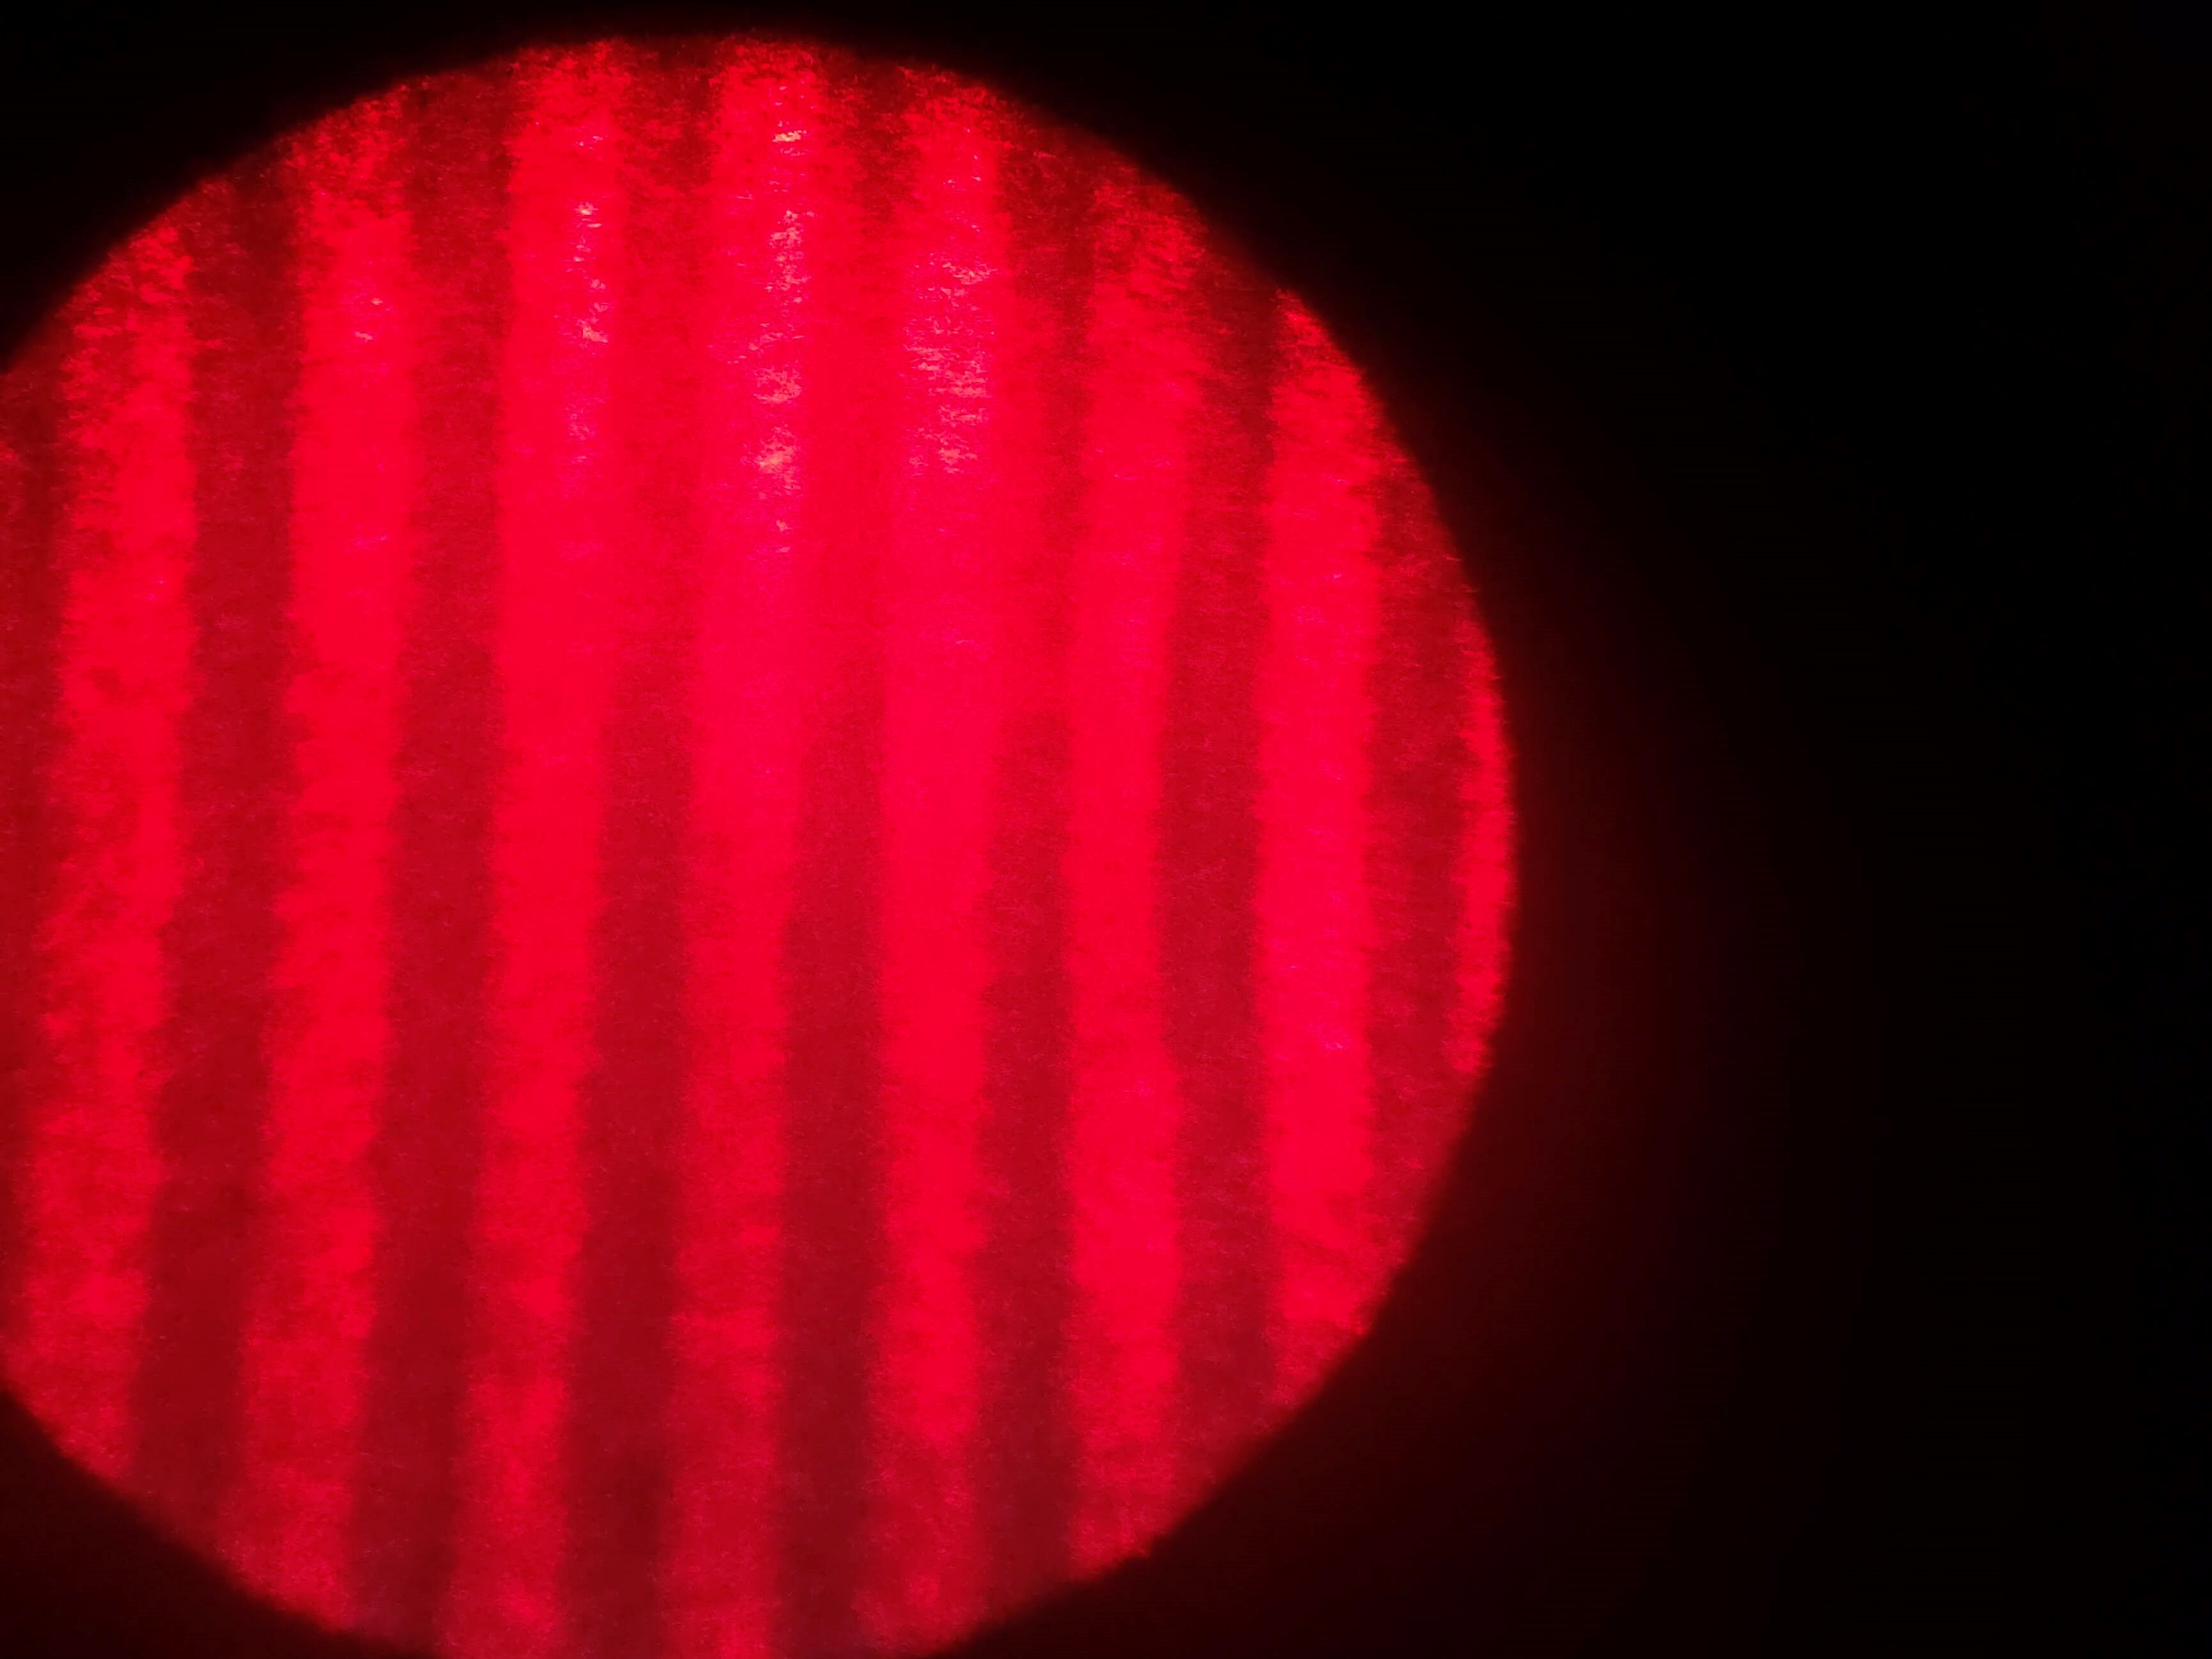
\includegraphics[width=0.45\textwidth]{二维-横狭缝-显微镜.jpg}}
            \caption{横狭缝光阑}
        \end{figure*}
        \begin{table}[h]
            \centering
            \begin{tabular}{|c|c|c|c|}
                \hline
                光阑形状 & 起点位置$x/mm$ & 10个条纹后的位置$x'/mm$ & 条纹间距$d/mm$ \\
                \hline
                横狭缝 & 35.318 & 29.758 & 0.5593 \\
                \hline
            \end{tabular}
            \caption{横狭缝光阑条纹间距测量}
        \end{table}

        \item[(4)] 斜狭缝 \\
        在频谱面上放上沿二四象限的狭缝,在像面上可以观察到沿一三象限的条纹。测量条纹间距时,测出水平方向的条纹间距,再除以$\sqrt{2}$即可得到斜向的条纹间距。
        根据表10中的测量结果,条纹间距变为原来的$\frac{\sqrt{2}}{2}$,也就是说条纹的空间频率变为原来的$\sqrt{2}$倍。这是因为斜狭缝使得频谱面上通过的
        衍射光斑的间距变为$\sqrt{2}$倍,也就是说频谱面上的基频、2倍频、3倍频……的空间频率都变为了原来的$\sqrt{2}$倍。所以条纹的空间频率也变为了$\sqrt{2}$倍,
        也即条纹间距变为原来的$\frac{\sqrt{2}}{2}$
        \begin{figure*}[h]
            \centering
            \subfigure[光屏上的像]{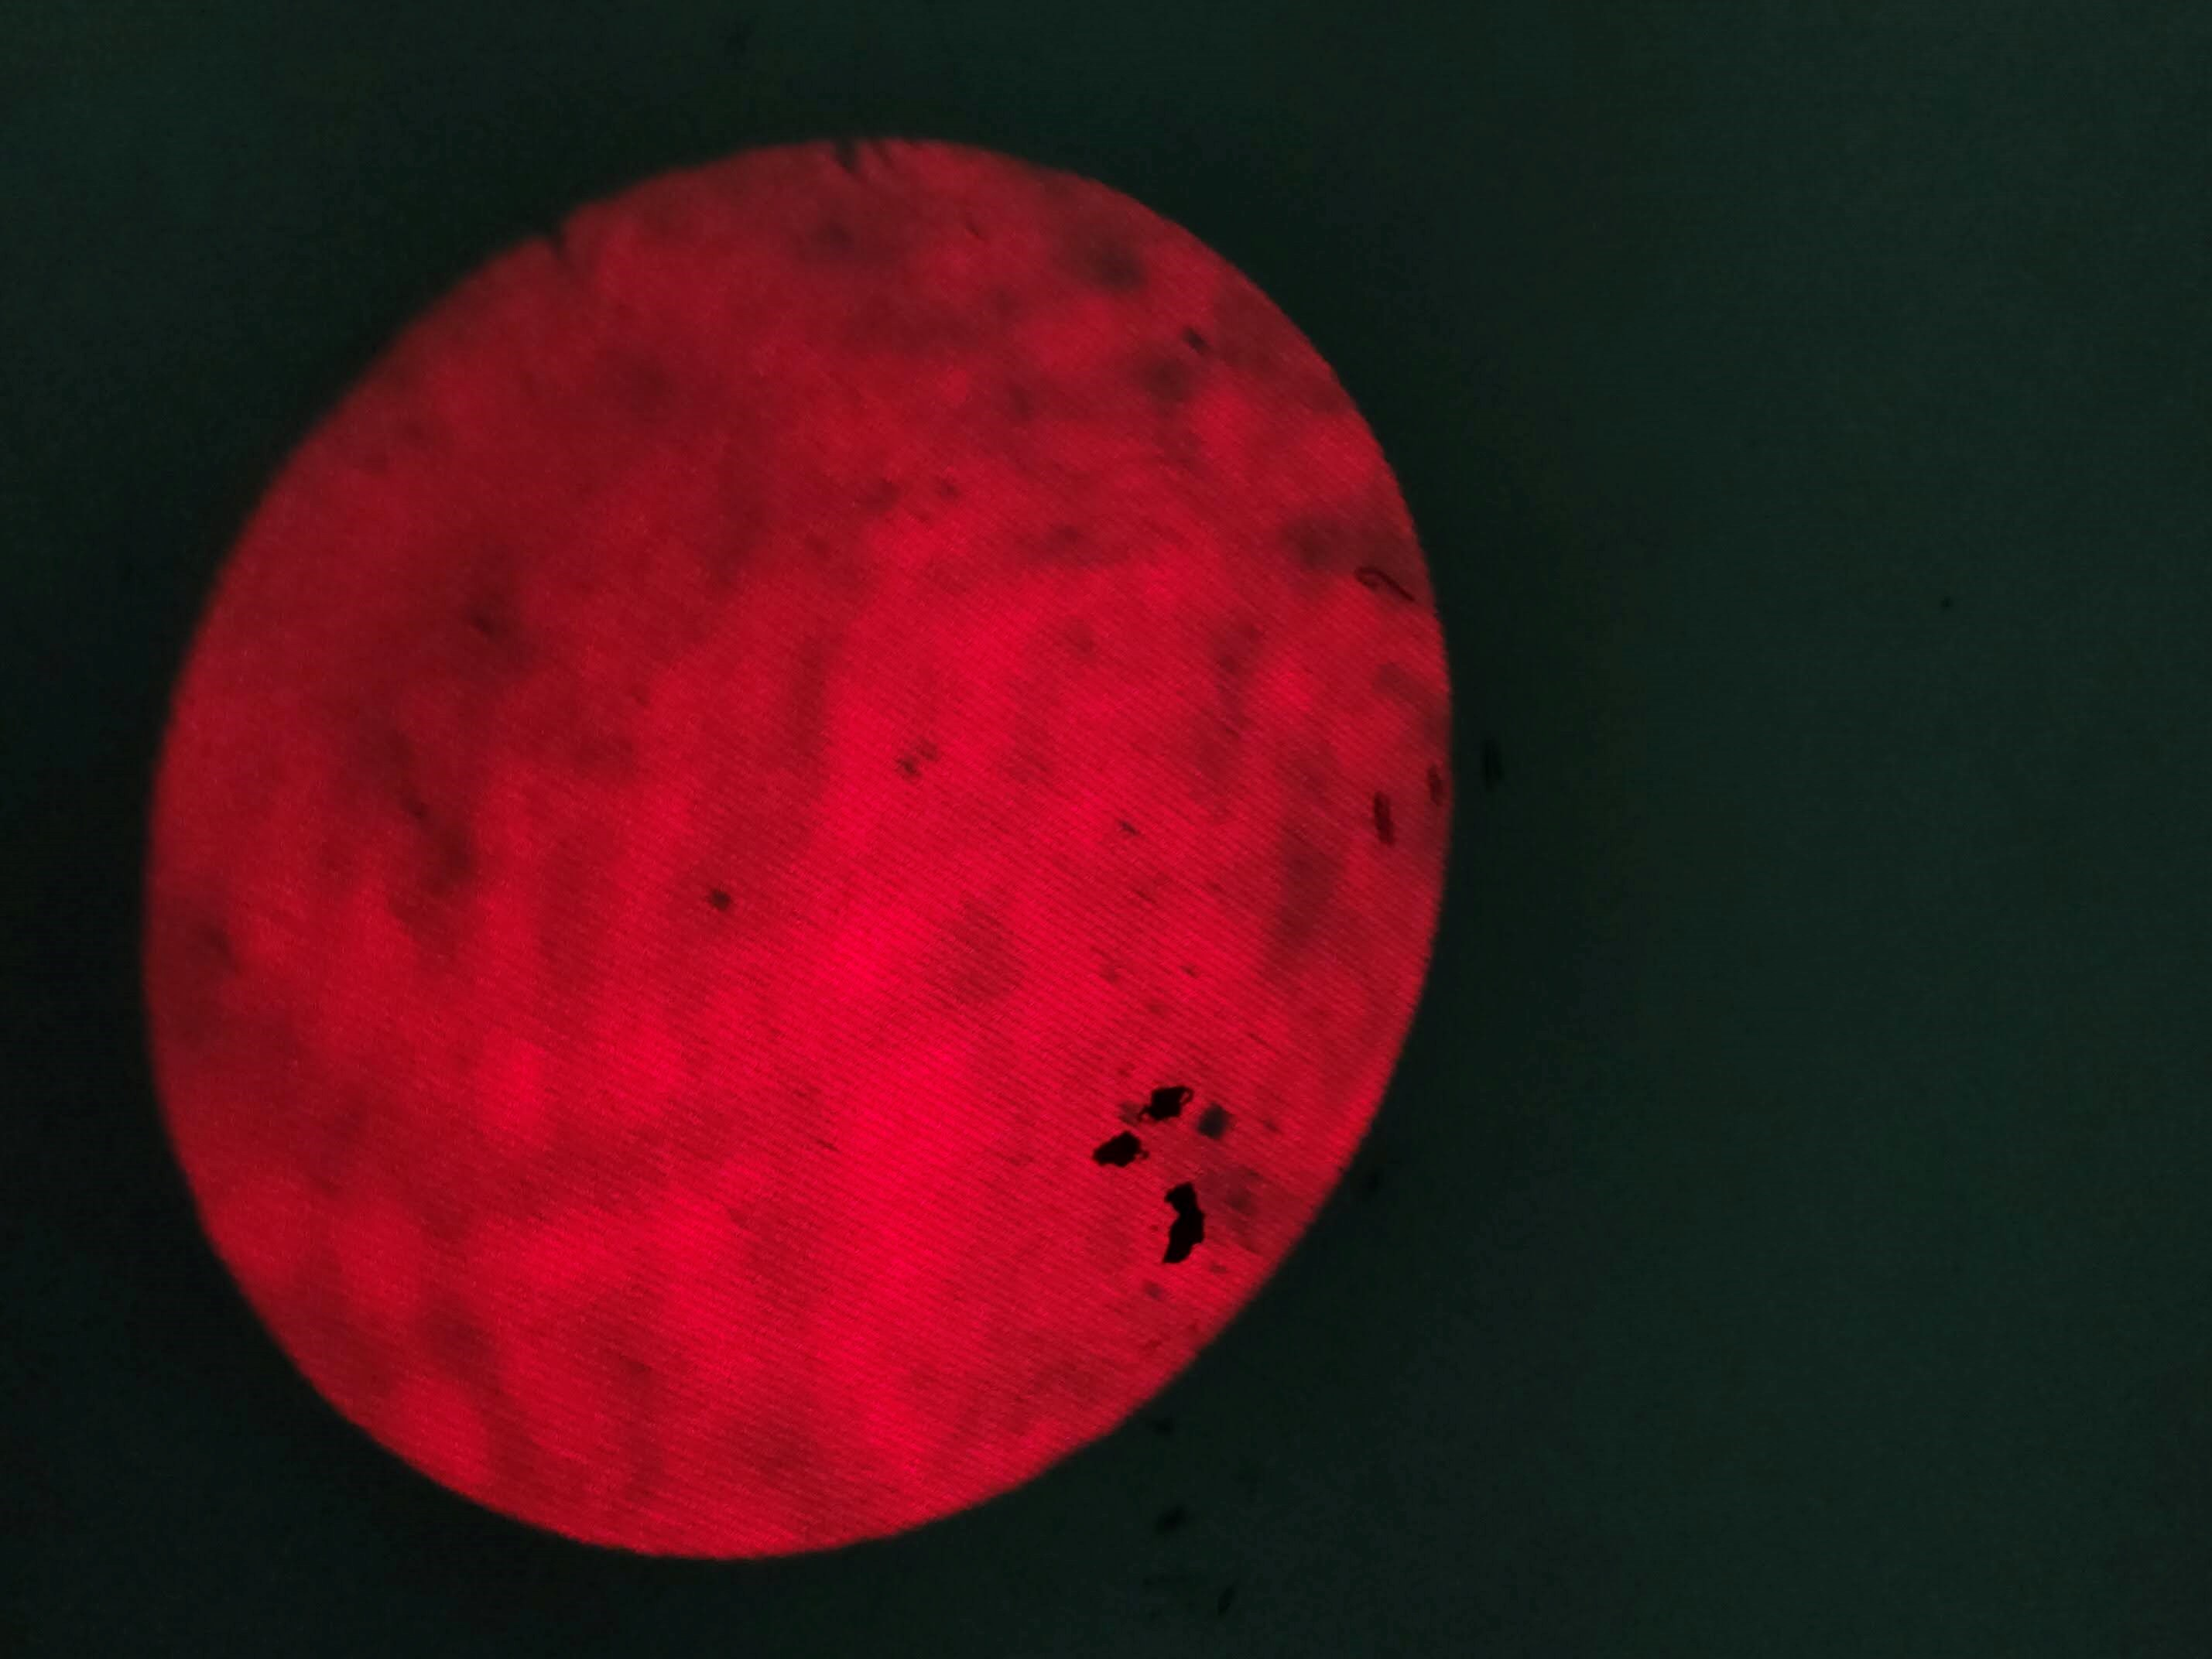
\includegraphics[width=0.45\textwidth]{二维-斜狭缝-屏.jpg}}
            \subfigure[显微镜中的像]{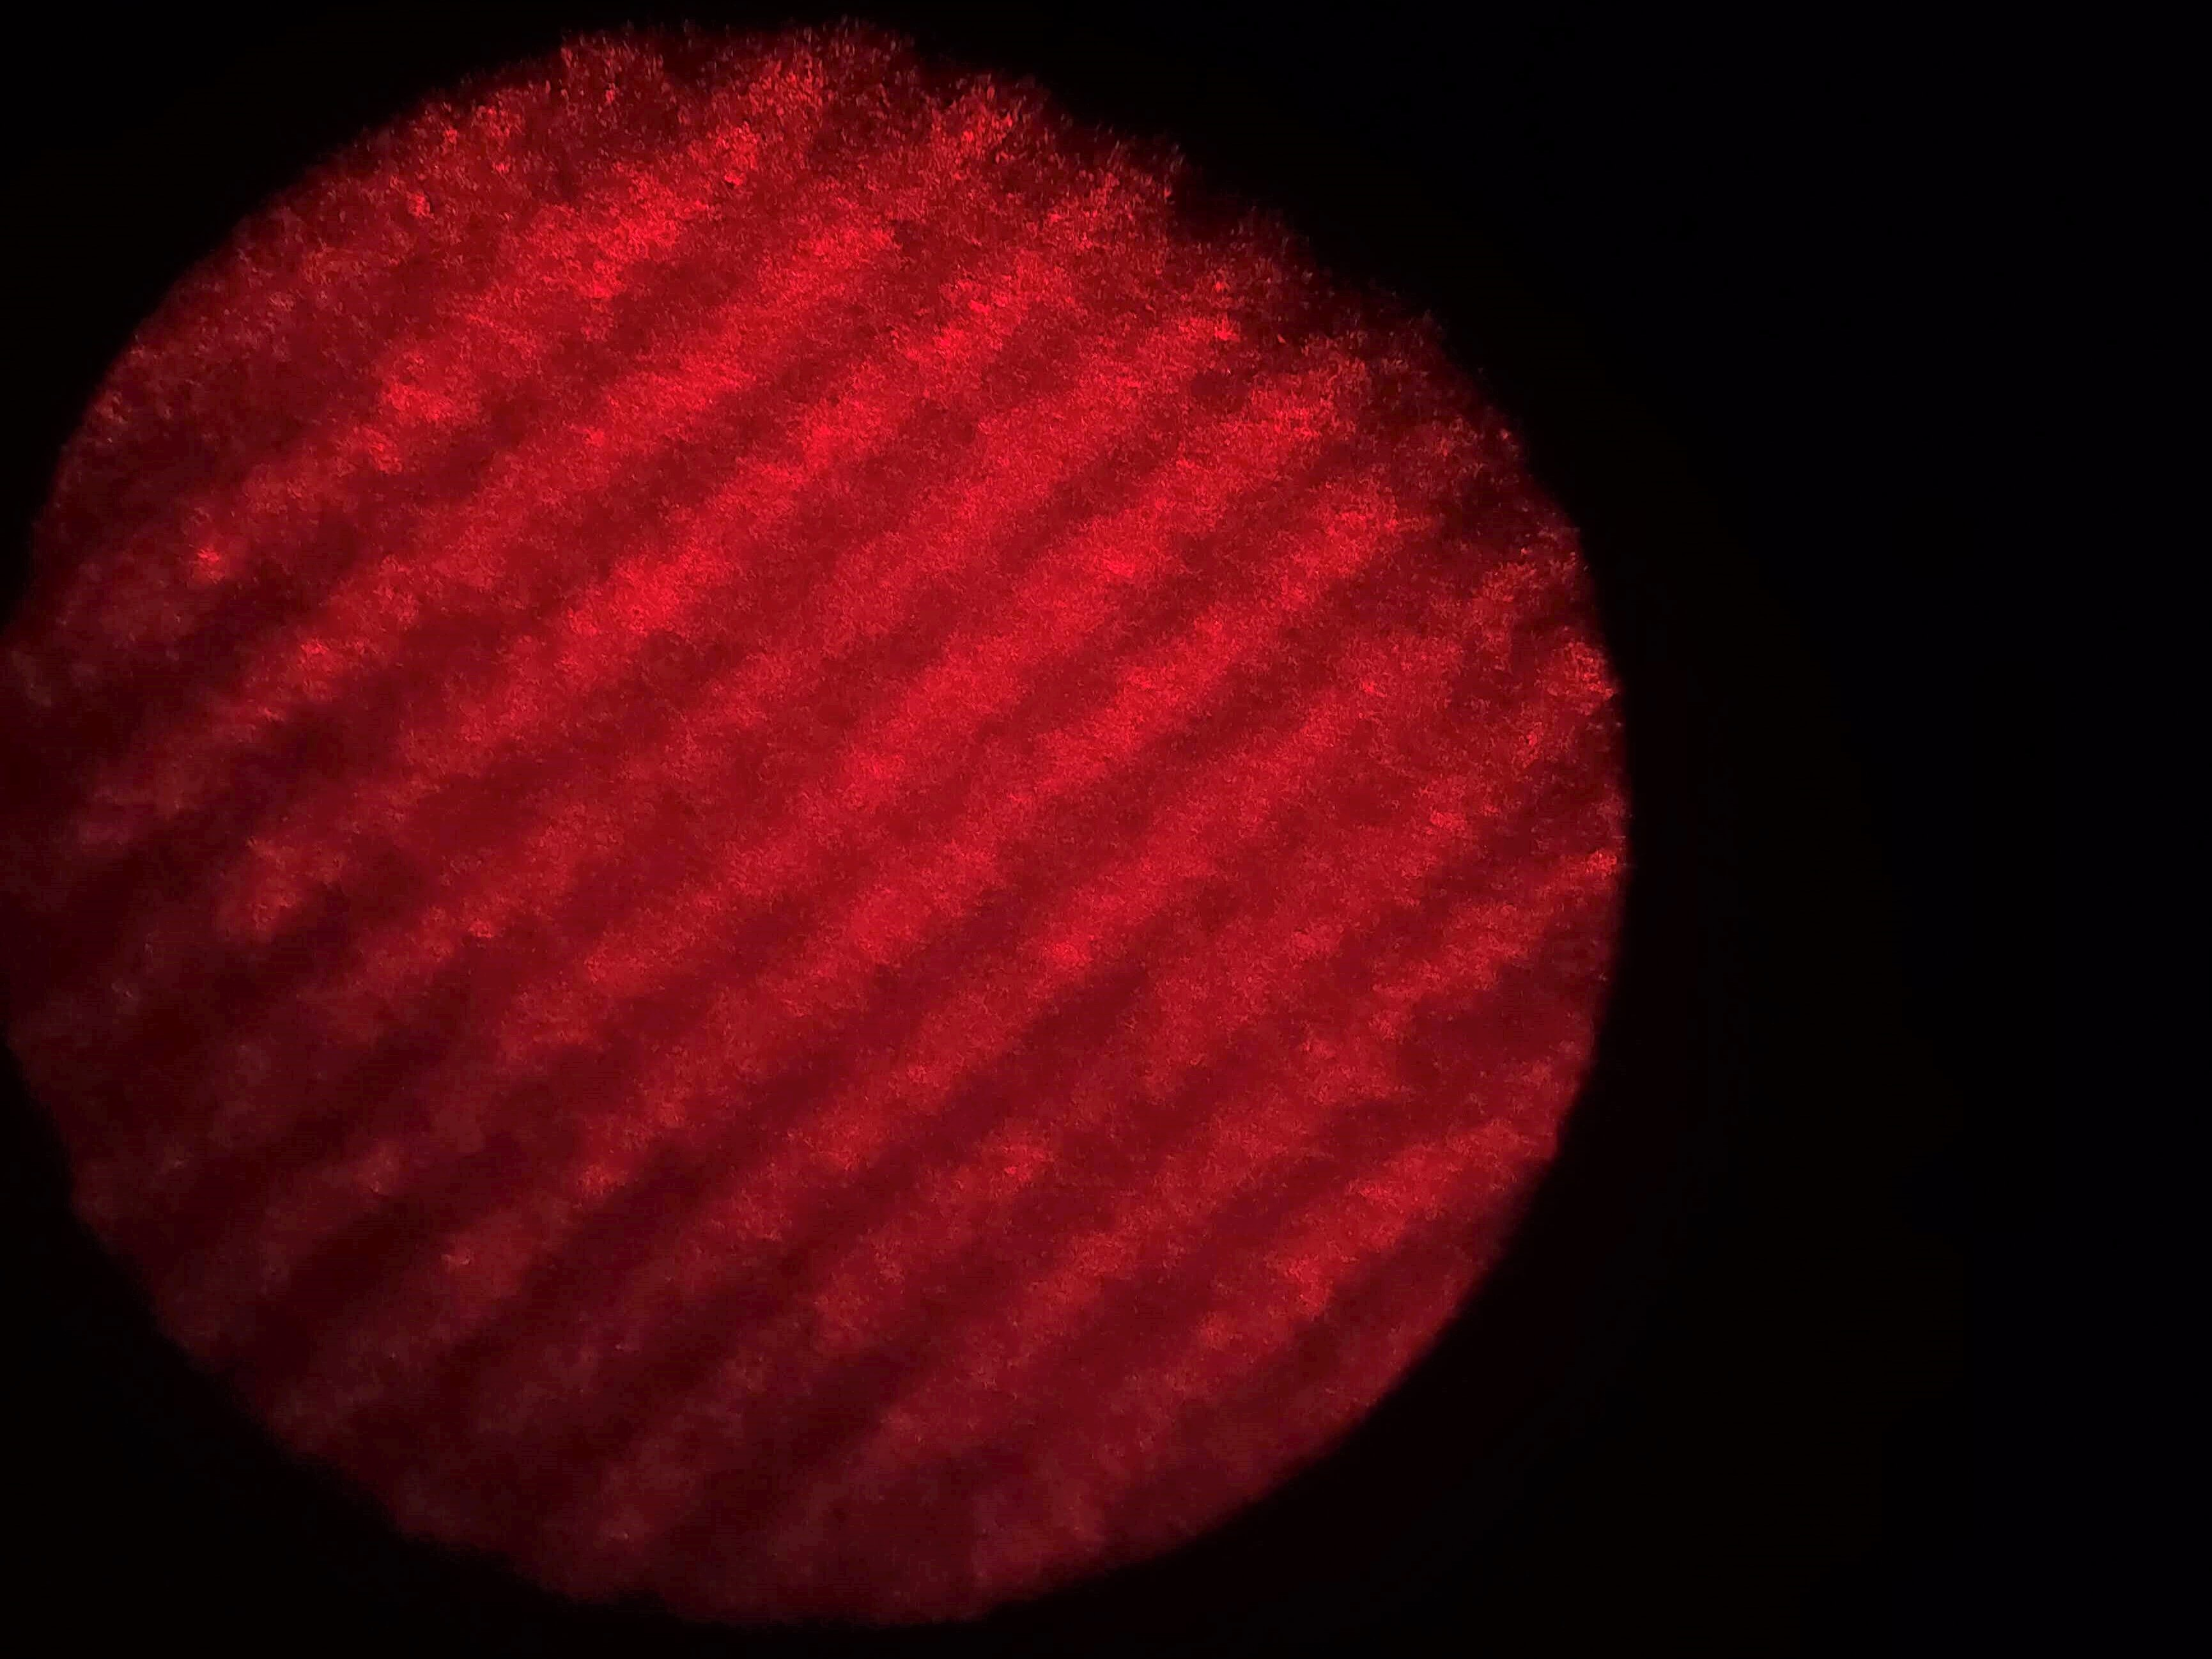
\includegraphics[width=0.45\textwidth]{二维-斜狭缝-显微镜.jpg}}
            \caption{斜狭缝光阑}
        \end{figure*}
        \newpage
        \begin{table}[h]
            \centering
            \begin{tabular}{|c|c|c|c|}
                \hline
                光阑形状 & 起点位置$x/mm$ & 10个条纹后的位置$x'/mm$ & 条纹间距$d/mm$ \\
                \hline
                斜狭缝 & 28.558 & 23.100 & 0.3859 \\
                \hline
            \end{tabular}
            \caption{斜狭缝光阑条纹间距测量}
        \end{table}
    \end{enumerate}

    \subsection{高低通滤波}
    \subsubsection{“光”字成像}
    将一个透明的“光”字与二维正交光栅重叠在一起作为物,透过光栅成像。在频谱面上除了观察到光栅频谱的点阵外,
    还能看到水平和竖直的两条亮线。这是“光”字所成的频谱。相较于周期性的光栅,“光”字本身不是周期的,因此其频谱是连续的,
    所以在频谱面上形成了水平竖直两条亮线。像面上可以看到“光”字的轮廓已经构成它的网格状条纹。

    \begin{figure*}[h]
        \centering
        \subfigure[频谱面上的像]{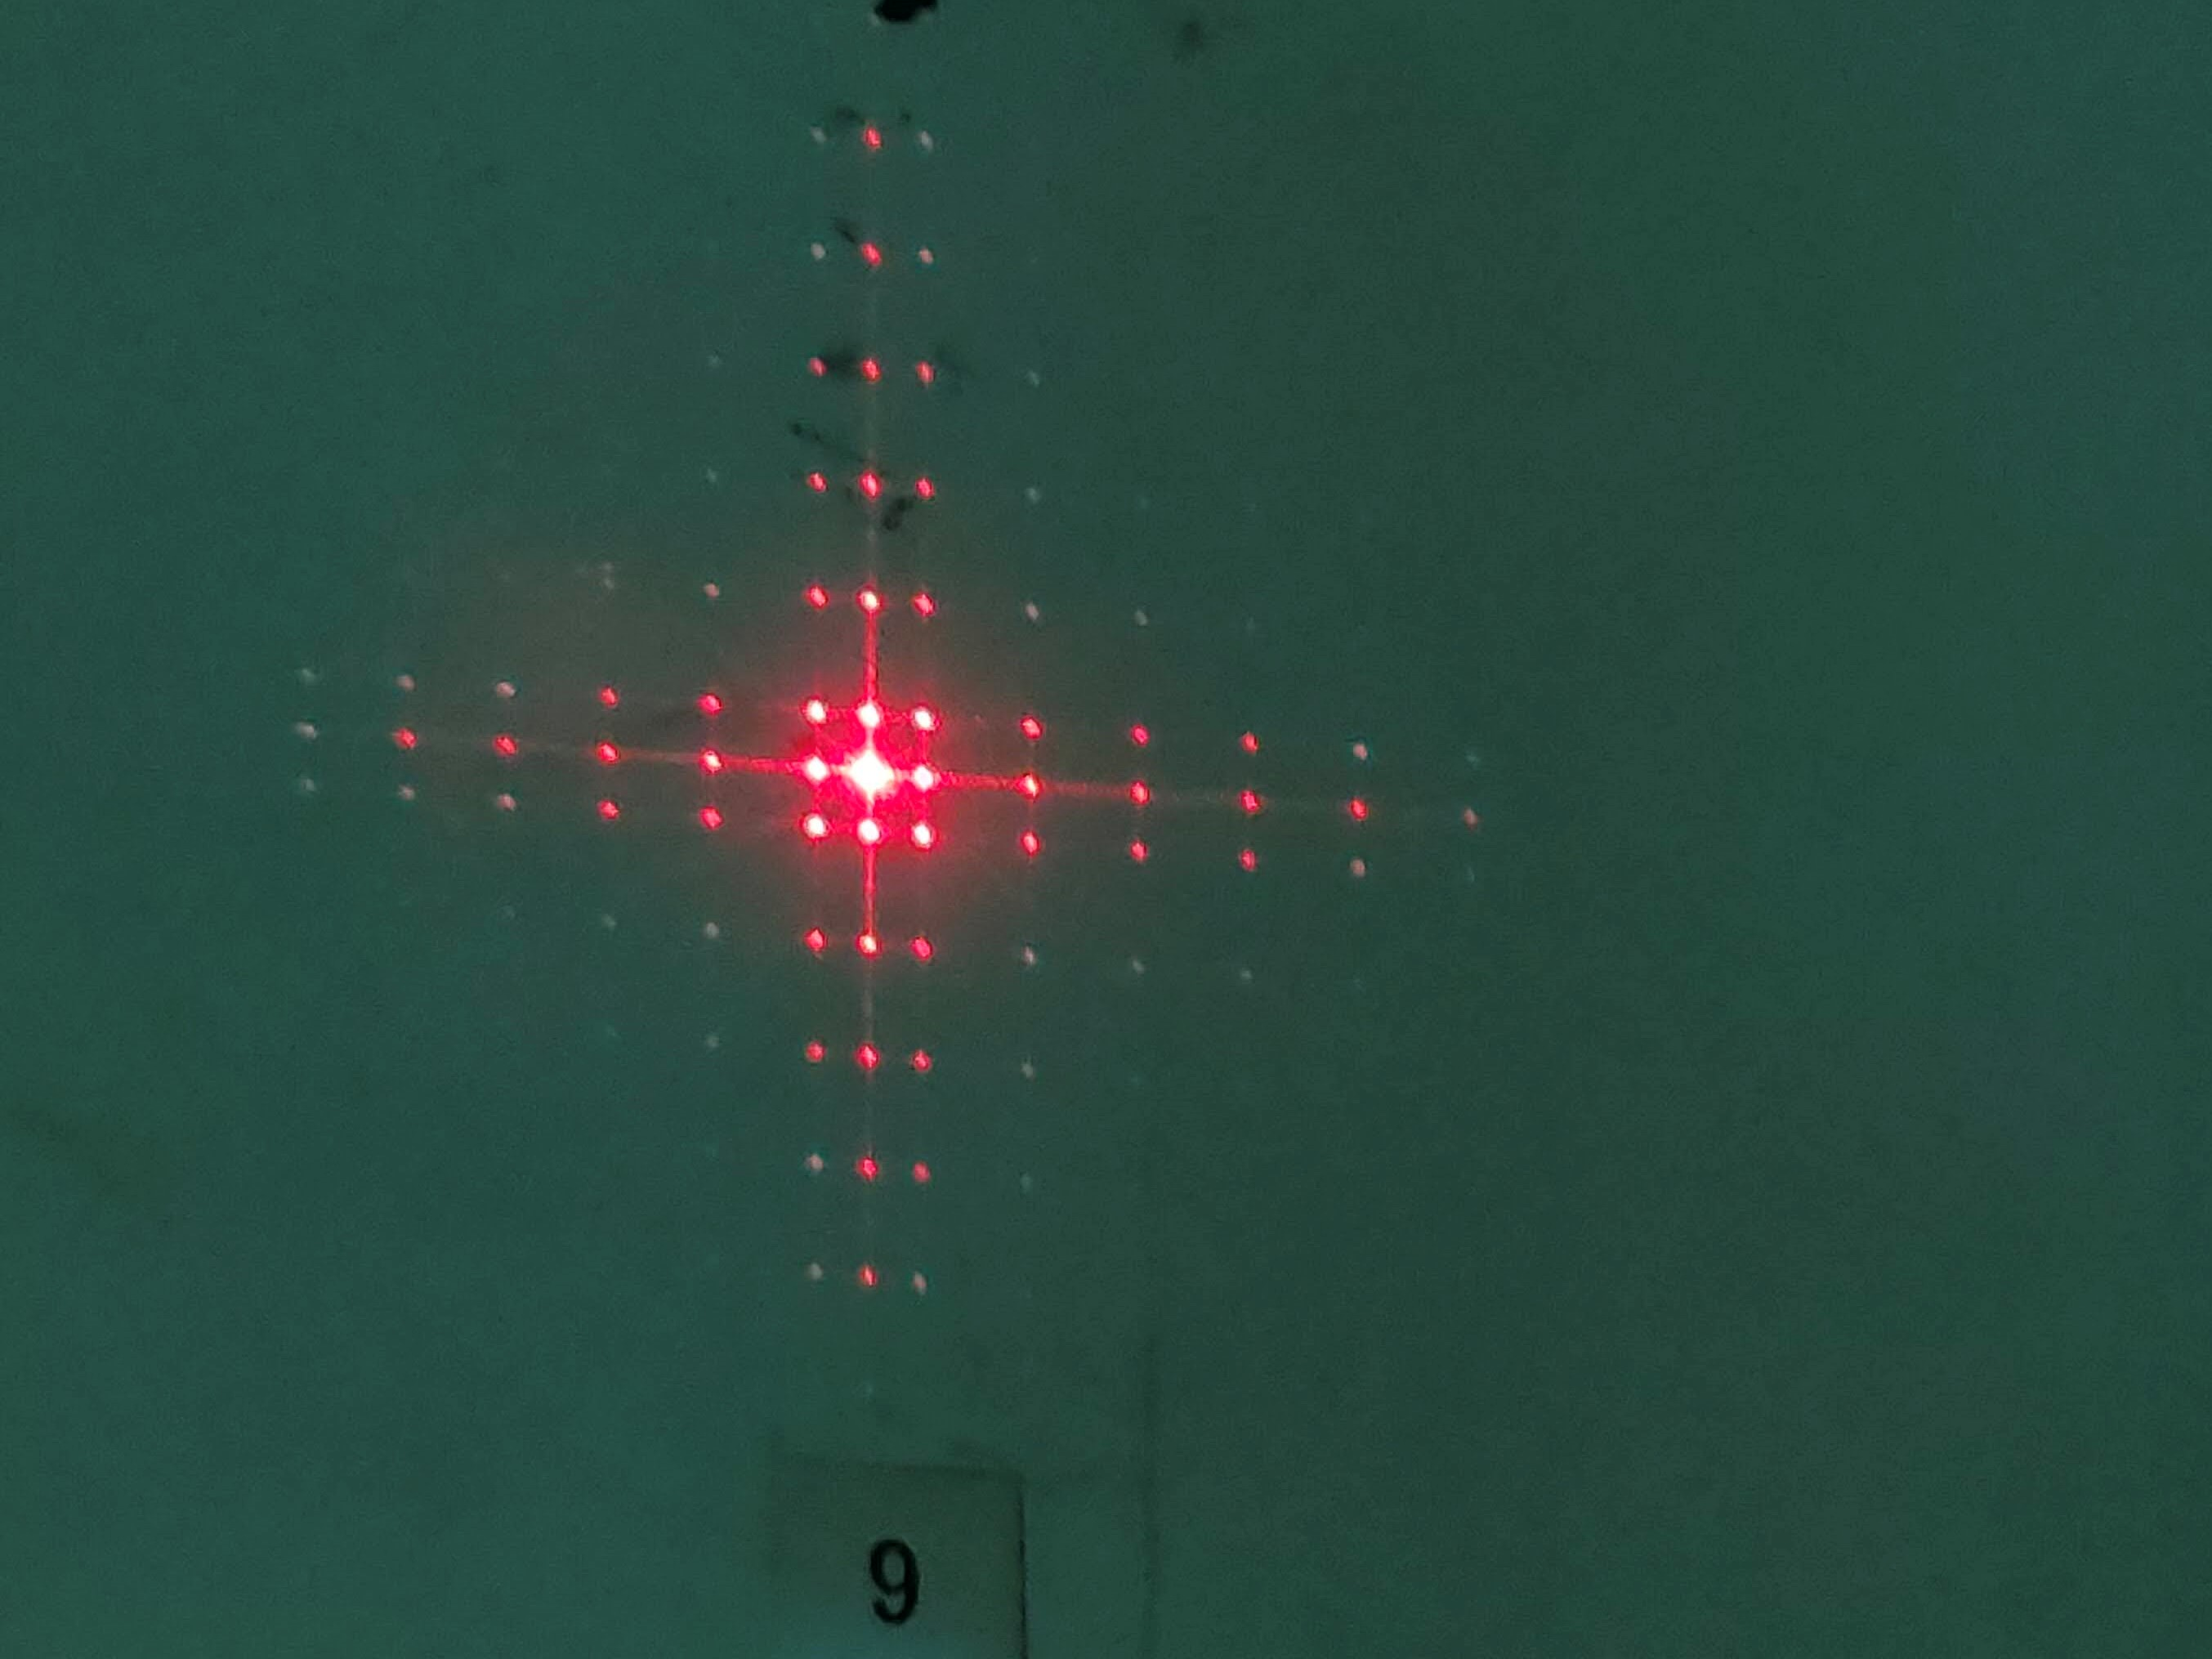
\includegraphics[width=0.45\textwidth]{光字频谱面.jpg}}
        \subfigure[像面上的像]{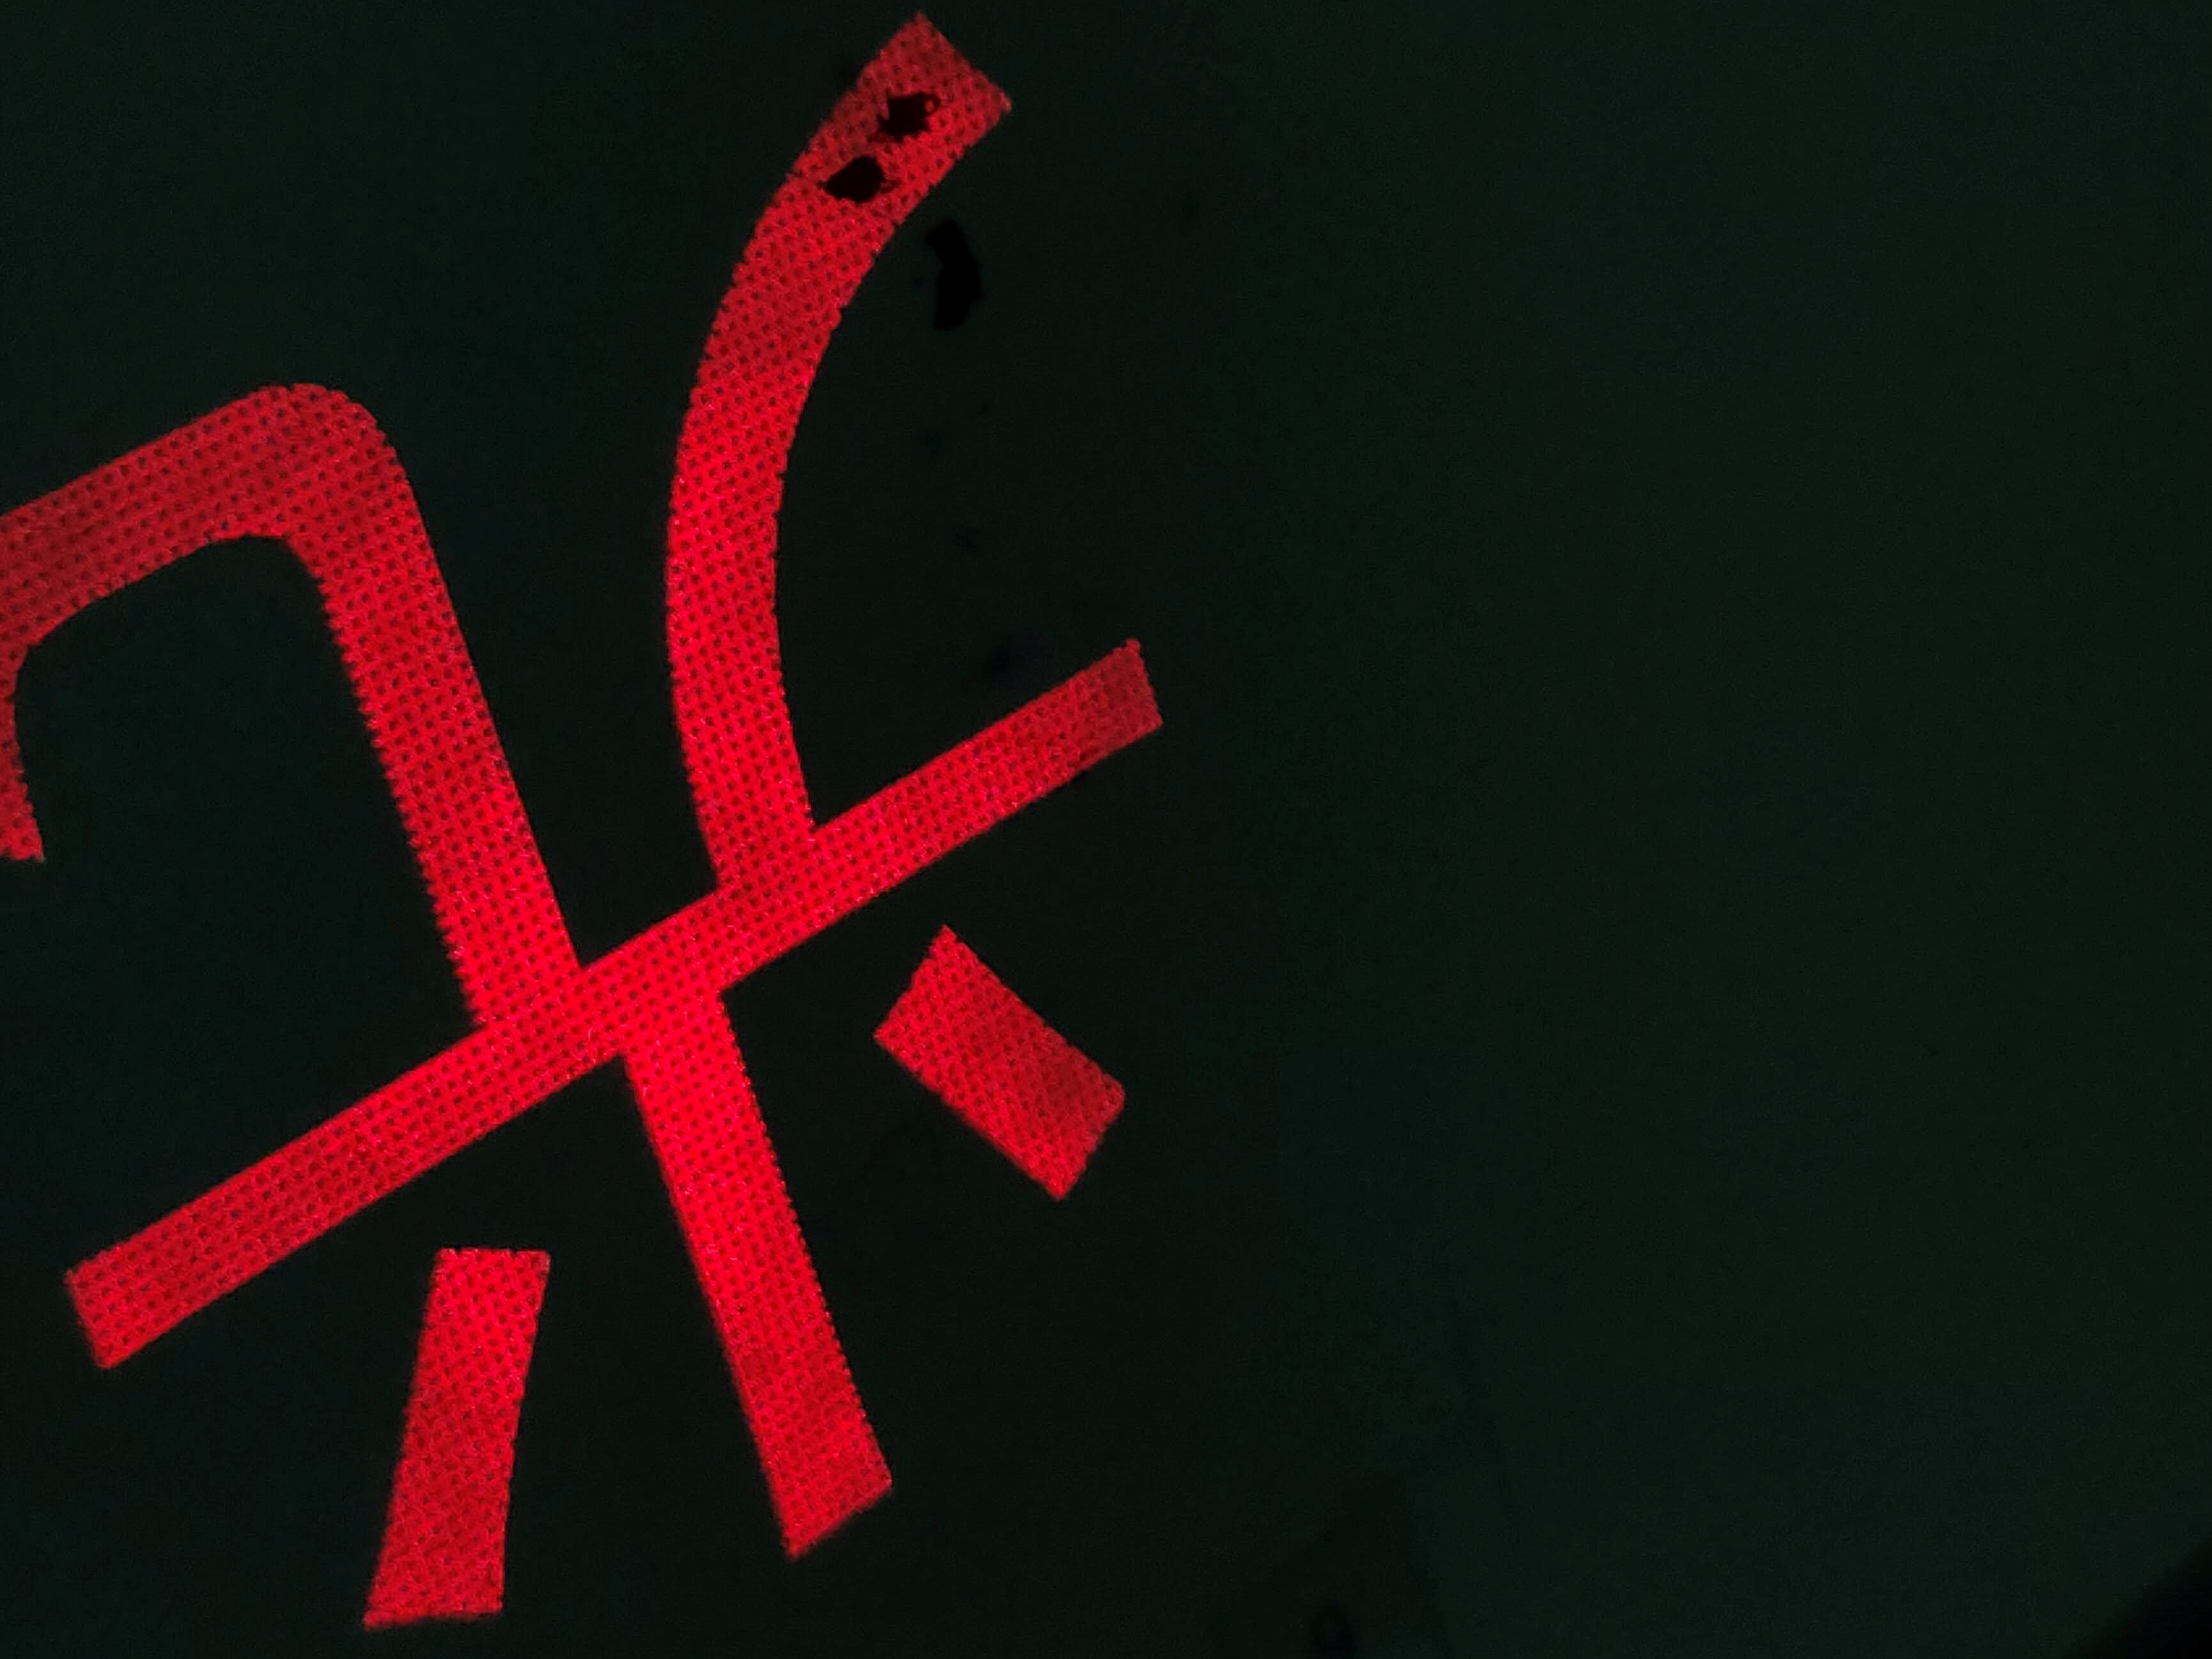
\includegraphics[width=0.45\textwidth]{光字像面.jpg}}
        \caption{“光”字成像}
    \end{figure*}

    \subsubsection{低通滤波}
    在频谱面上放置一圆孔光阑,当孔径$\phi = 1mm$和孔径$\phi = 0.3mm$时,像面上的像分别如图11(a)和图11(b)所示。
    可以看到在用圆孔光阑进行低通滤波时,“光”字变得模糊了,且小孔时比大孔更加模糊。此外两个孔进行滤波后,网格状条纹都消失不见了。
    这是因为小孔只能允许光栅的频谱中的0级光斑通过,不具有任何光栅的频谱信息,因此看不到光栅的条纹。而“光”字的频谱是连续谱,小孔还是可以允许一定的频率通过的,
    但由于通过的都是低频信息,因此“光”字也变得模糊了。
    \begin{figure*}[h]
        \centering
        \subfigure[频谱面上的像]{
\includegraphics[width=0.45\textwidth]{光字大孔像面.jpg}}
        \subfigure[像面上的像]{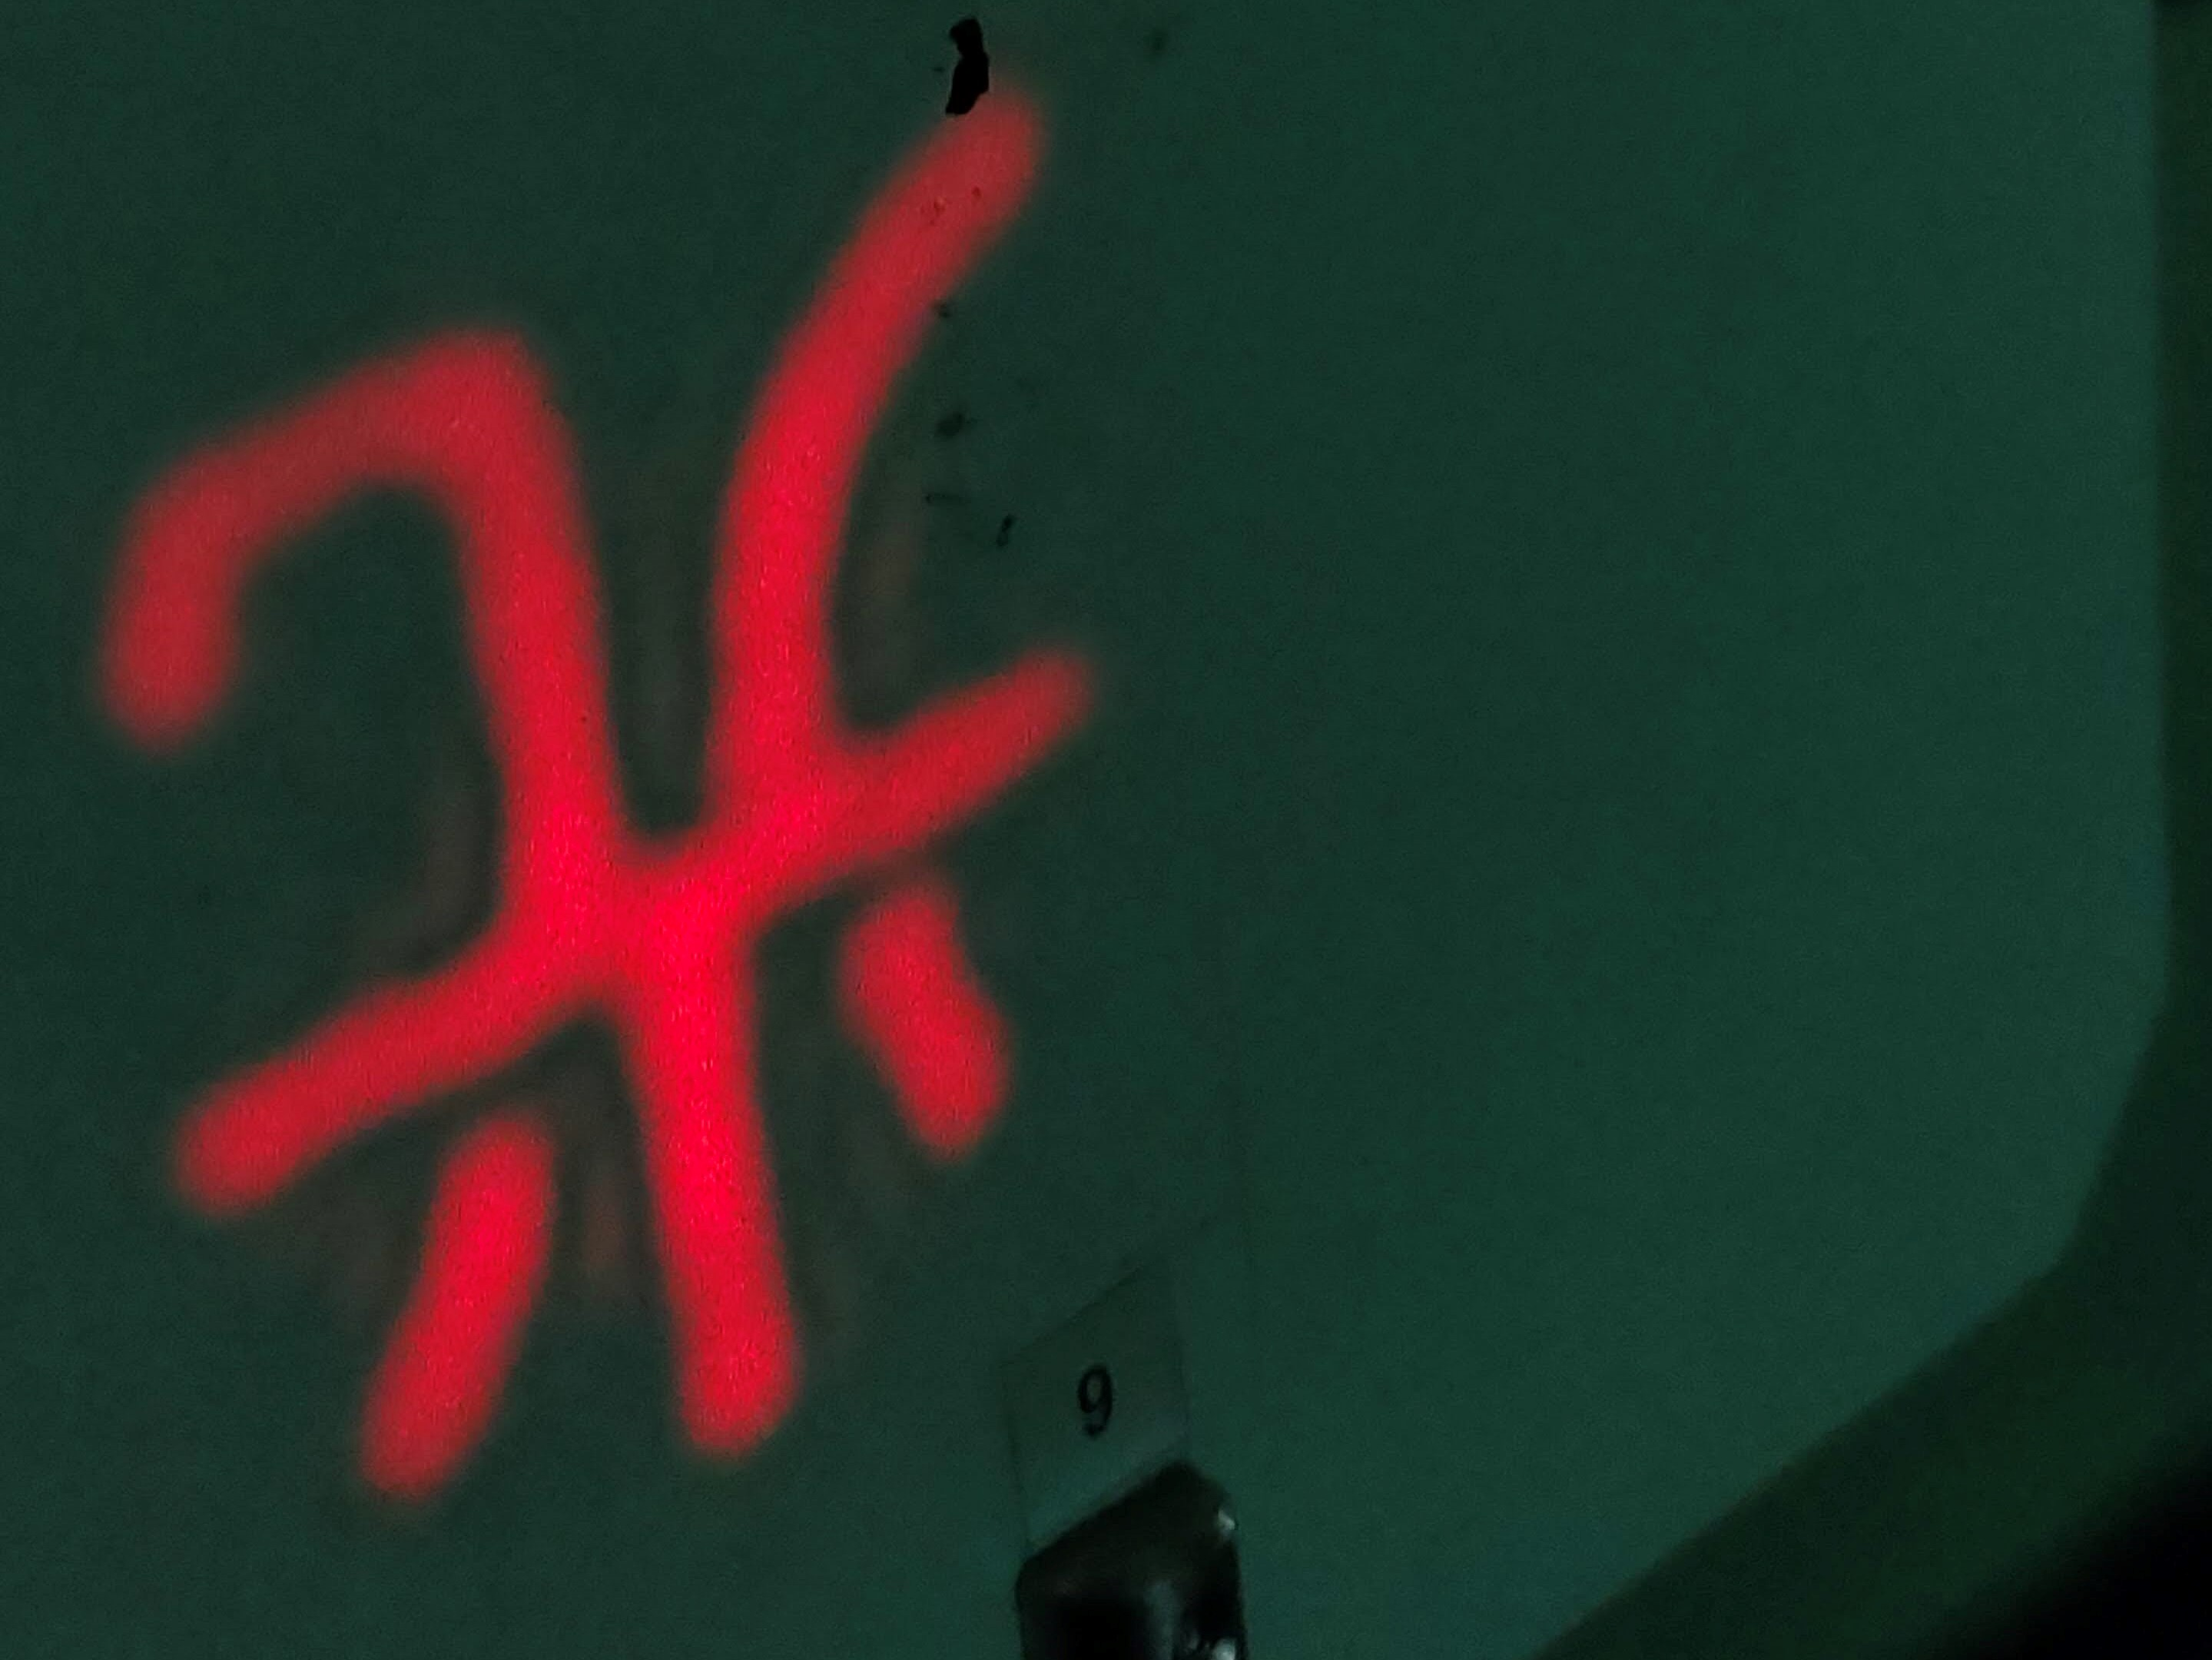
\includegraphics[width=0.45\textwidth]{光字小孔像面.jpg}}
        \caption{“光”字低通滤波}
    \end{figure*}

    实验中,正交光栅的空间频率为12/mm,因此,如果要使得像面上看不到网格,需要使得频谱面上的基频及所有倍频信息被滤除。频谱面上0级衍射点到1级衍射点(基频)
    的距离为$x=f\lambda F=12\times 632.8\times 10^{-6} \times 250=1.90mm$,所以当小孔光阑的半径$r < 1.90mm$时,网格就会消失。

    对于“光”字我们也可以做类似的处理,其笔画宽度为0.5mm,因此我们可以将其空间频率视为2/mm,所以如果小孔光阑的半径$r<2\times 632.8\times 10^{-6} \times 250 =0.32mm$

    如果将圆孔光阑做一平移,使不在光轴上的一个点(如上方的1级衍射点)通过圆孔,在光屏上可以看到“光”字和网格状条纹,
    但条纹和“光”字都没有未进行滤波时清晰。这是因为不在光轴上的点(1级衍射点)作为基频,包含一定的细节信息,因此能在
    光屏上看到正交光栅的轮廓,但由于更高频的细节信息丢失了,因此光栅的轮廓不是非常清晰。(由于实验操作疏忽,本环节忘记拍照了)

    \subsubsection{“十”字成像与高通滤波}
    将一个透光的“十”字作为物,通过透镜成像,可以在像面上看到它的像如图13(b)所示。其频谱面上是由一个中心亮斑和两条正交亮线组成的(图13(a)),这是因为“十”字
    不是周期的,因此其频谱也是连续谱。
    \begin{figure*}[h]
        \centering
        \subfigure[频谱面上的像]{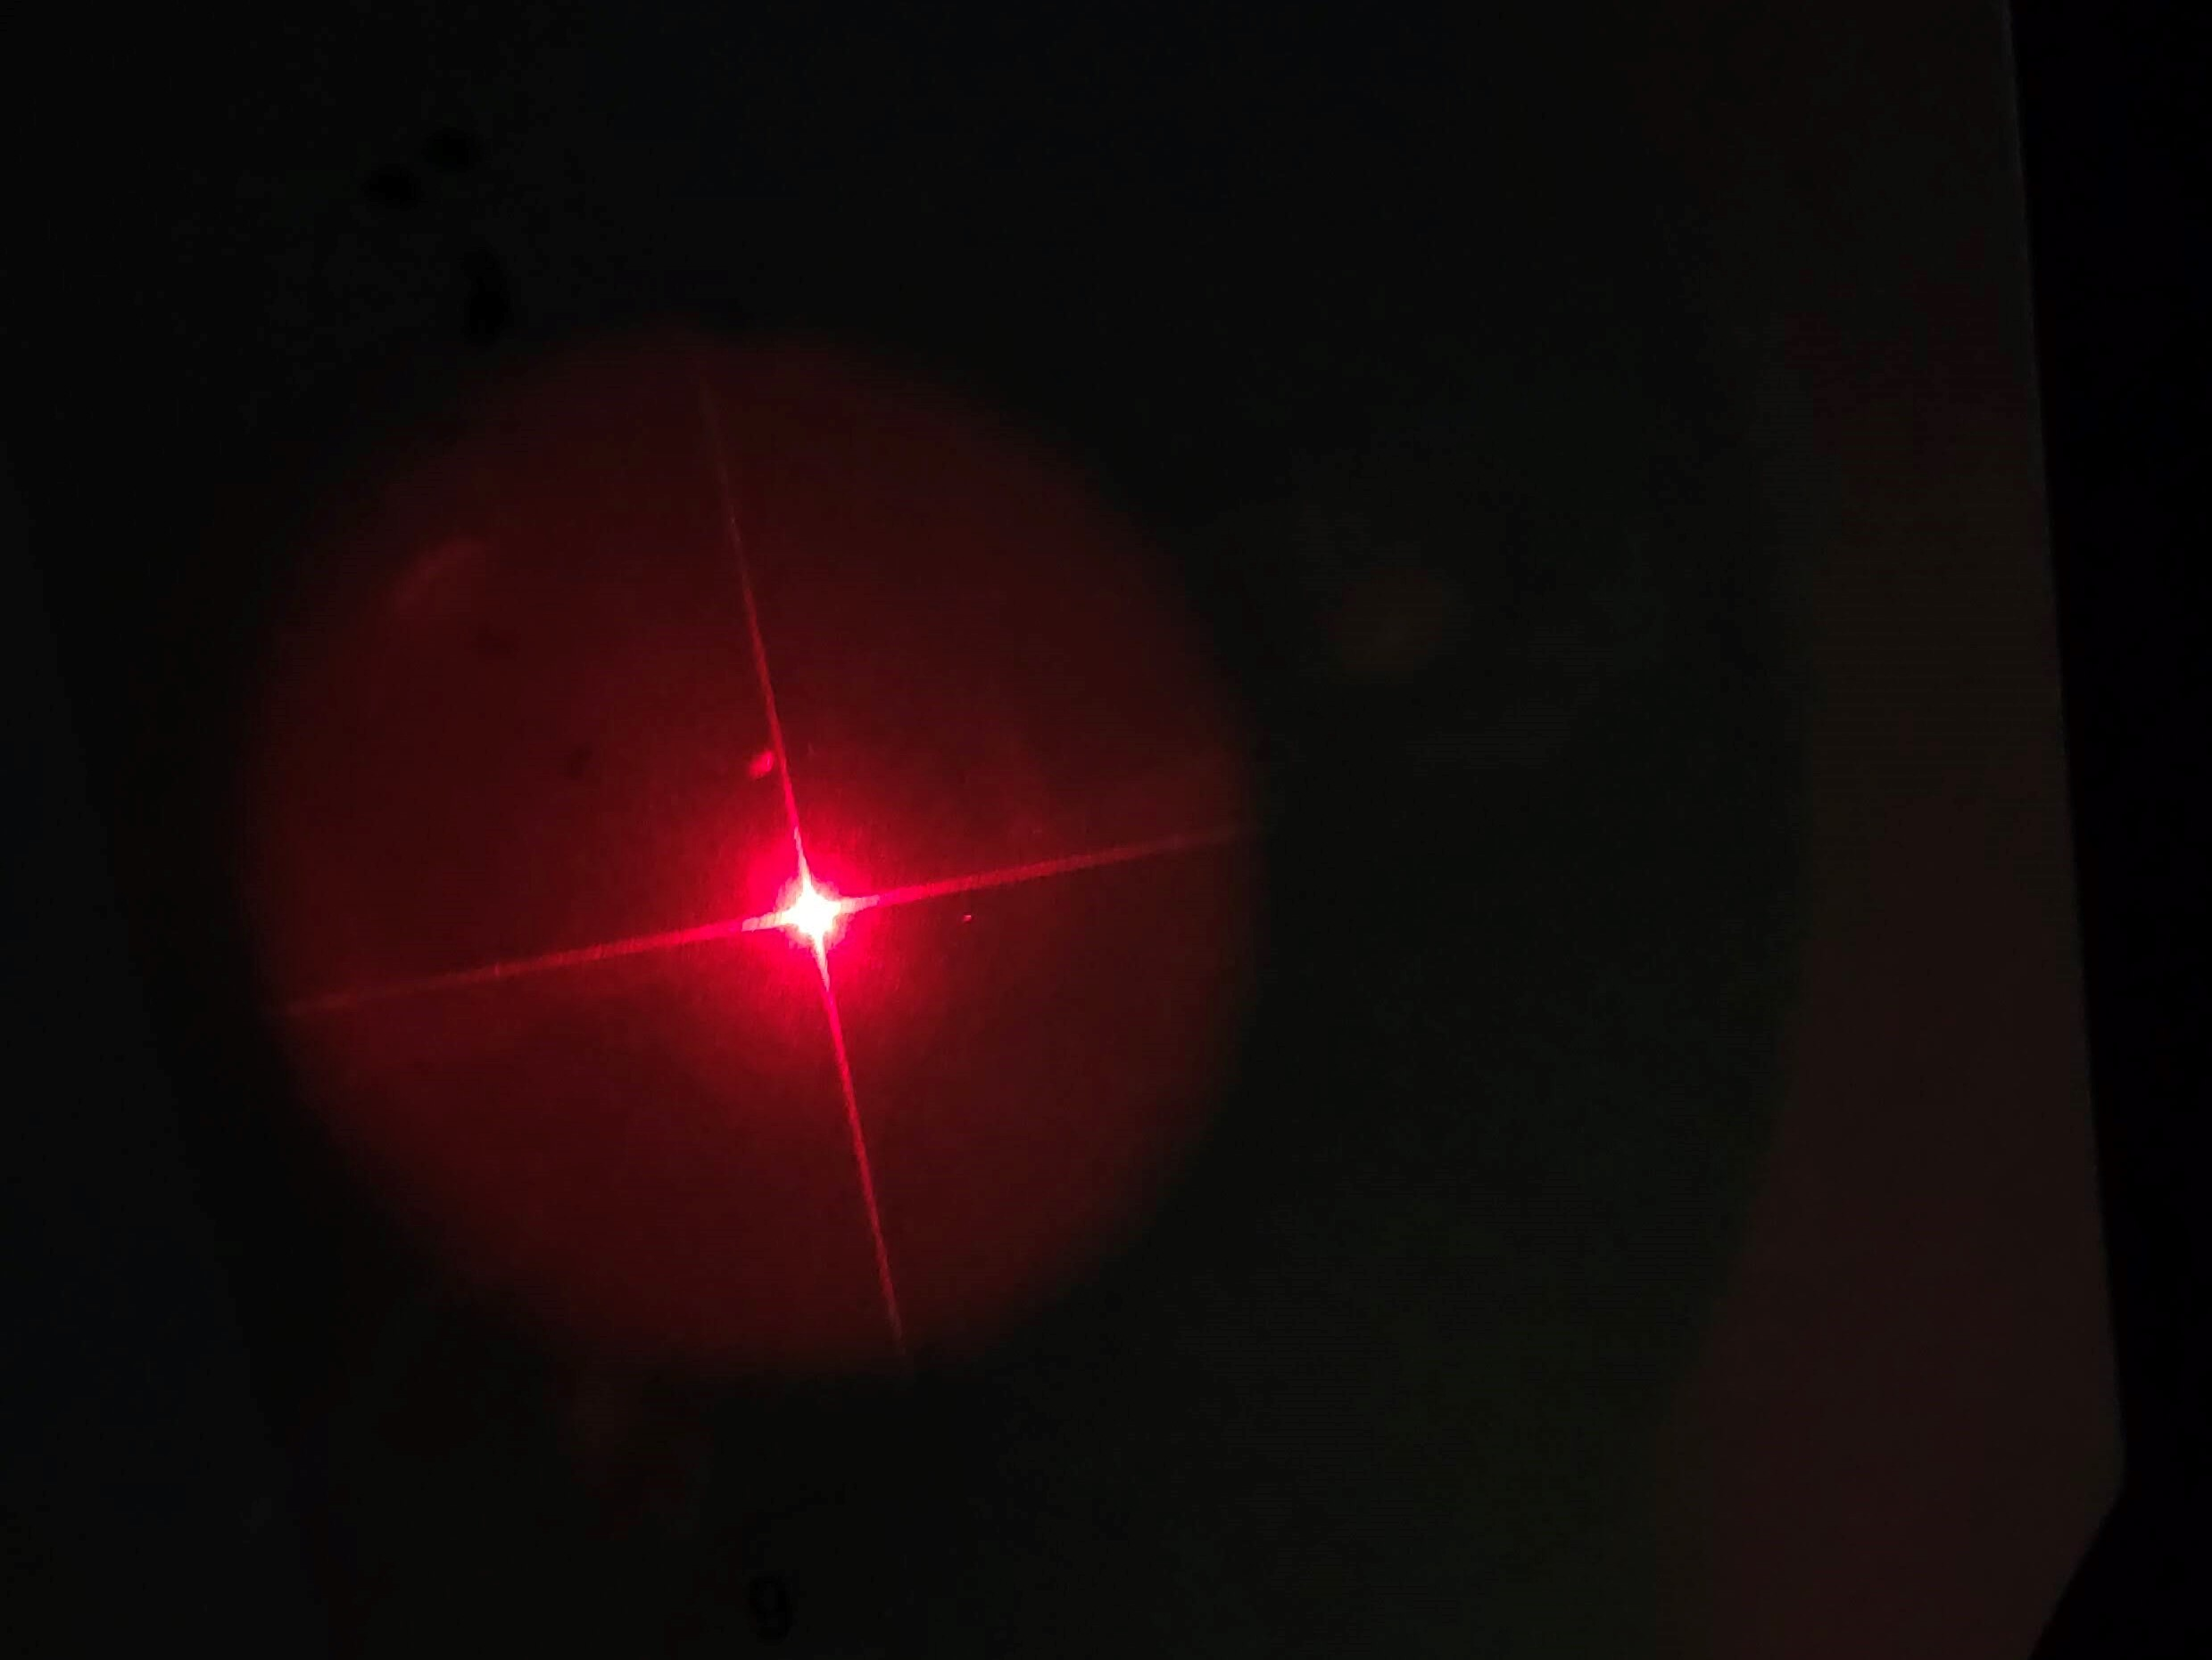
\includegraphics[width=0.45\textwidth]{十字频谱面.jpg}}
        \subfigure[像面上的像]{
\includegraphics[width=0.45\textwidth]{十字.jpg}}
        \caption{“十”字成像}
    \end{figure*}

    在频谱面上放一屏状光阑挡去空间频谱的中心部分,可以看到像面上的像如图14所示。可以看到整个“十”字都变暗了,
    但十字的轮廓却比较亮。这是因为空间频谱的中心部分主要提供均匀的本底和一定的低频信息,现在中心被挡掉了,就只剩下
    高频信息。由于像的轮廓大多是由低频信息组成的,而像的细节由高频信息组成,且相较于高频信息,低频信息亮度高一点,
    因此剩余的这部分高频信息里的低频部分提供了轮廓,高频部分提供了细节,故像的整体亮度下降了,但轮廓变亮了。
    \begin{figure*}[h]
        \centering
        \subfigure[频谱面上的像]{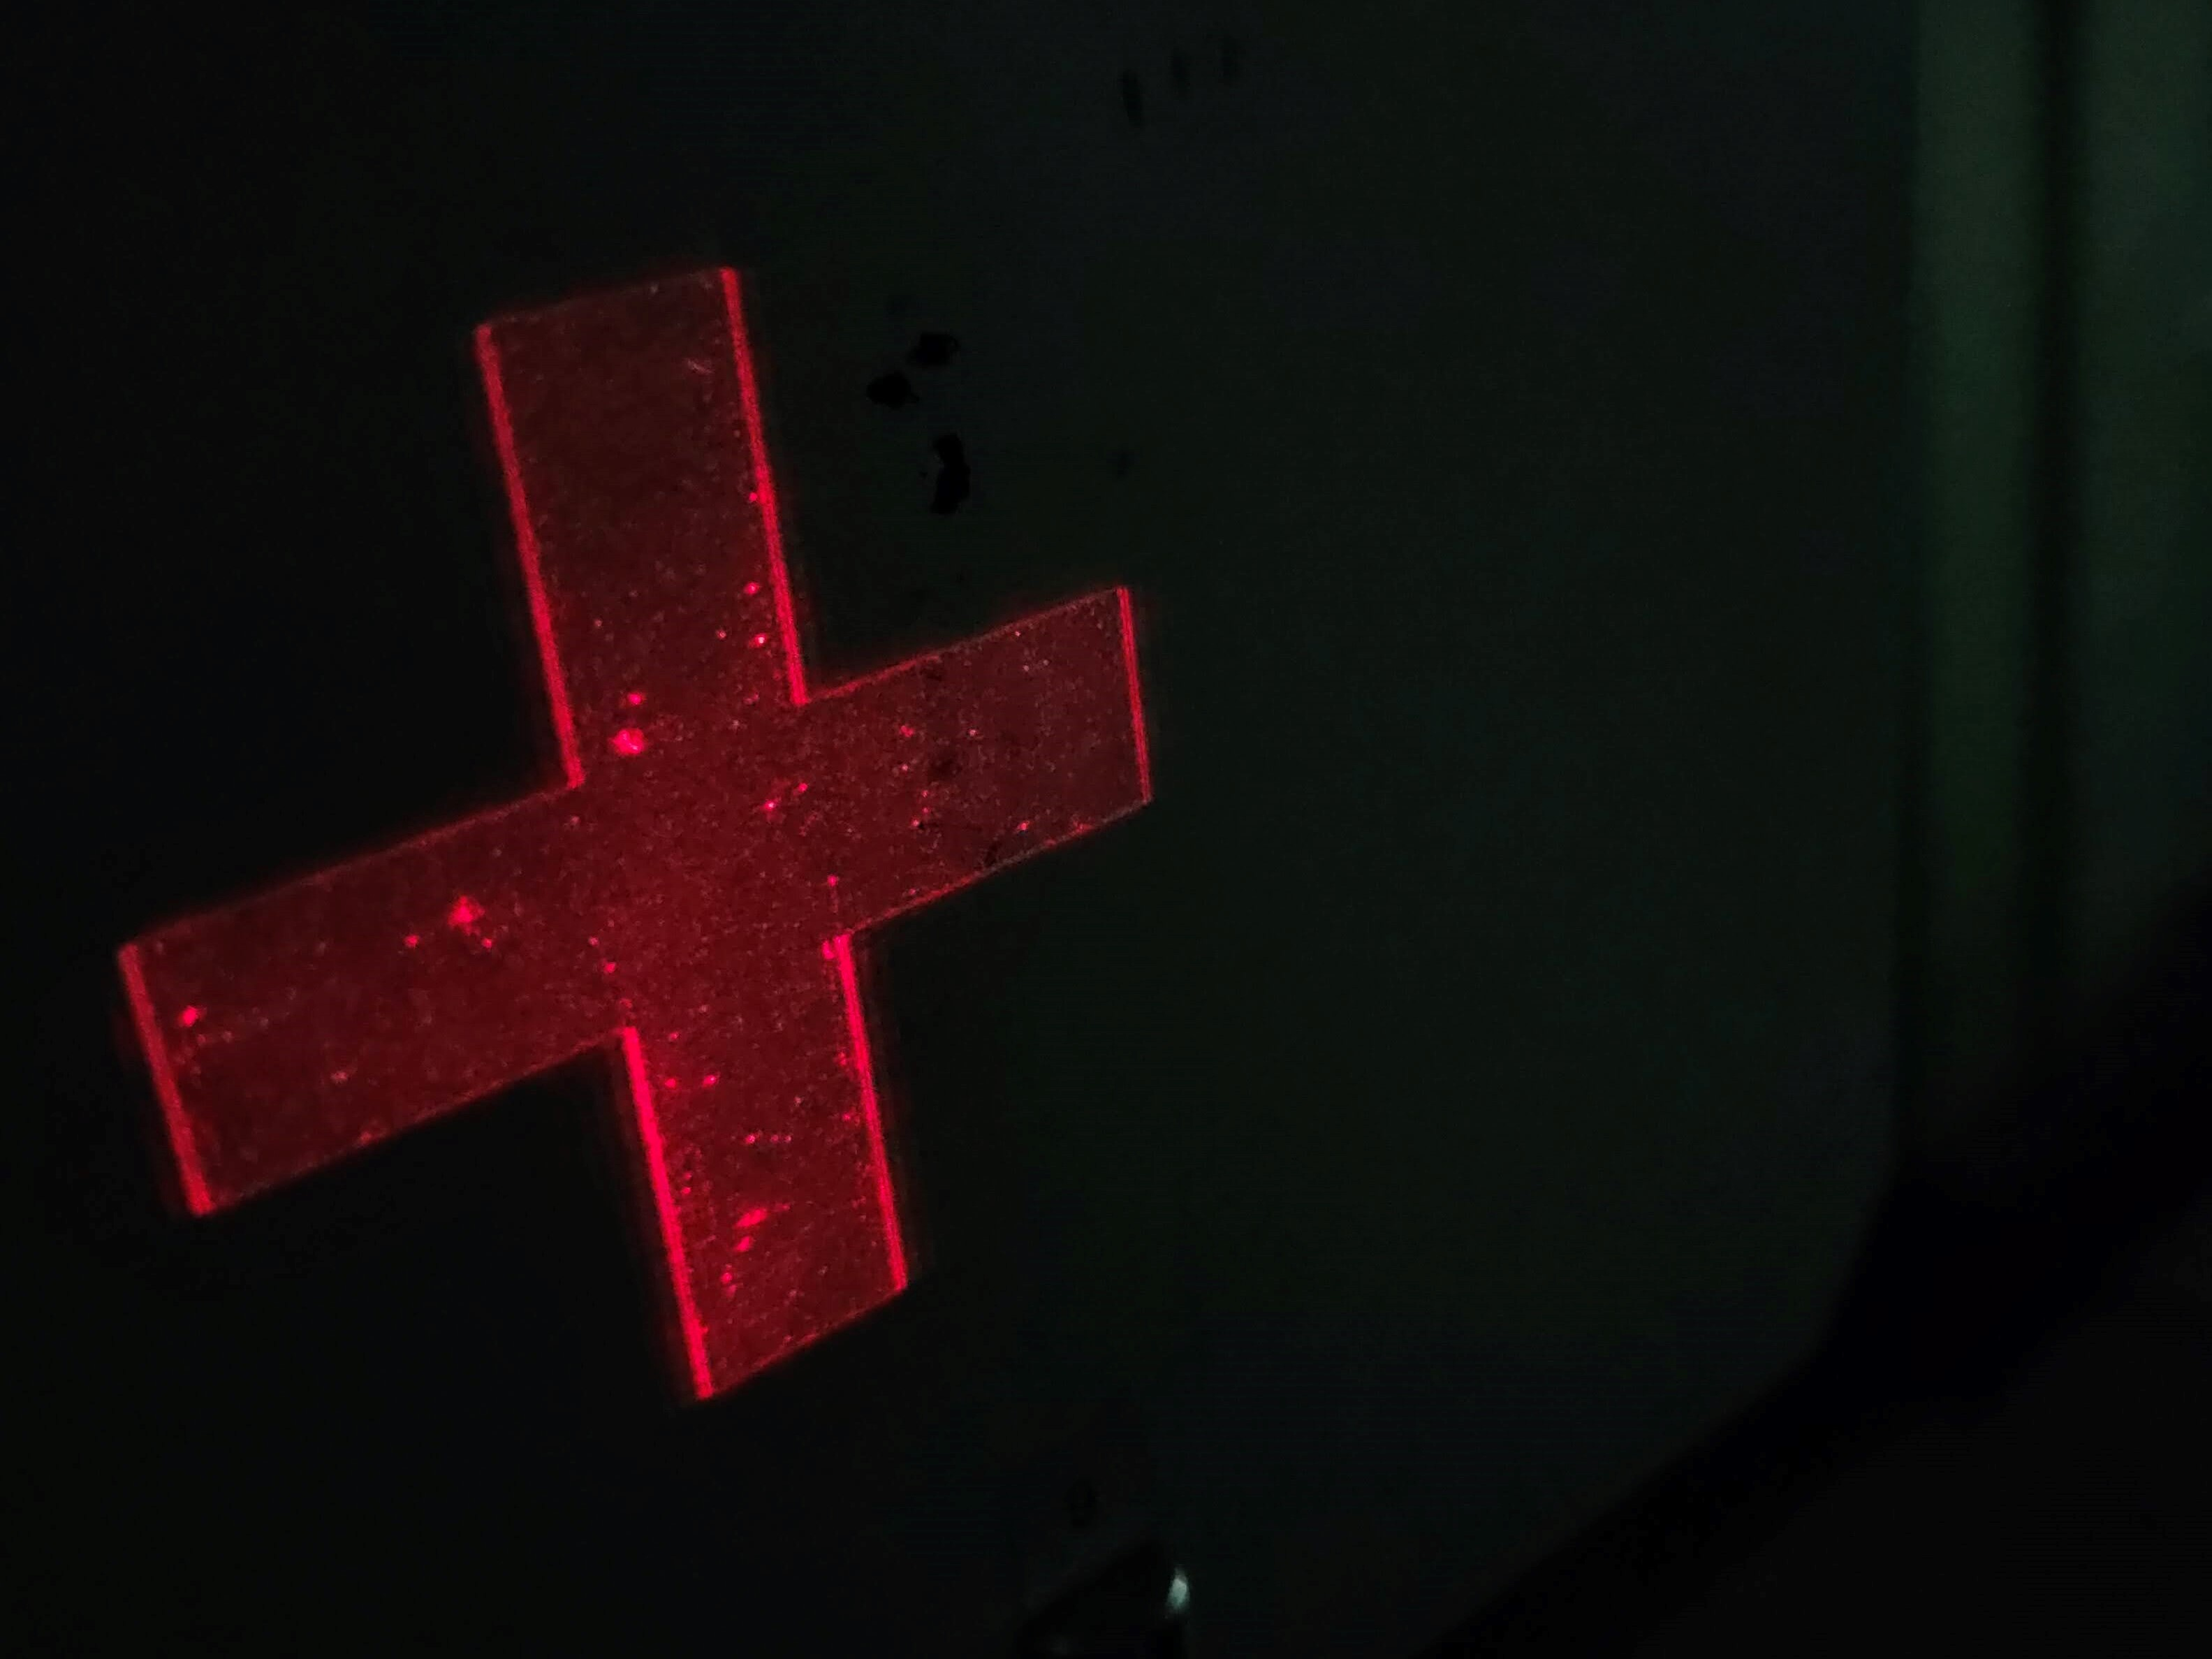
\includegraphics[width=0.45\textwidth]{十字中心挡光像面.jpg}}
        \caption{“十”字高通滤波}
    \end{figure*}

    \subsection{卷积现象的观察}
    将激光分别照在20/mm的二维正交光栅和200/mm的二维正交光栅上,观察其频谱面上的特征,可以看到其在频谱上的频谱都是点阵。
    而20/mm的光栅的频谱点阵更密一点,200/mm光栅的频谱点阵更稀疏一点。这是因为频谱面上的各级次衍射点到中心的距离与光栅的基频、2倍频、3倍频……的空间频率成正比。
    20/mm的光栅的空间频率是200/mm的光栅的空间频率的$\frac{1}{10}$,因此点阵要更加密集一点。

    将两光栅重叠,可以看到在200/mm光栅形成的较稀疏的点阵上,每个衍射点周围都有一些小的、较密集的点阵。转动200/mm的光栅,
    较稀疏的大点阵会随之转动而小点阵不动,且转动的过程中亮度会发生周期性变化,亮的时候很亮,暗的时候几乎消失。而转动20/mm的光栅,
    小点阵会随着转动而大点阵不动,且转动的过程中亮度变化不是十分明显。这些现象是两组光栅的傅里叶变换进行卷积的结果。
\end{document}